% Options for packages loaded elsewhere
\PassOptionsToPackage{unicode}{hyperref}
\PassOptionsToPackage{hyphens}{url}
\PassOptionsToPackage{dvipsnames,svgnames,x11names}{xcolor}
\documentclass[
  british,
  10pt,
  a4paper,
]{article}
\usepackage{xcolor}
\usepackage[margin=22mm]{geometry}
\usepackage{amsmath,amssymb}
\setcounter{secnumdepth}{-\maxdimen} % remove section numbering
\usepackage{iftex}
\ifPDFTeX
  \usepackage[T1]{fontenc}
  \usepackage[utf8]{inputenc}
  \usepackage{textcomp} % provide euro and other symbols
\else % if luatex or xetex
  \usepackage{unicode-math} % this also loads fontspec
  \defaultfontfeatures{Scale=MatchLowercase}
  \defaultfontfeatures[\rmfamily]{Ligatures=TeX,Scale=1}
\fi
\usepackage{lmodern}
\ifPDFTeX\else
  % xetex/luatex font selection
  \setmainfont[]{DejaVu Serif}
  \setsansfont[]{DejaVu Sans}
  \setmonofont[]{DejaVu Sans Mono}
  \setmathfont[]{DejaVu Math TeX Gyre}
\fi
% Use upquote if available, for straight quotes in verbatim environments
\IfFileExists{upquote.sty}{\usepackage{upquote}}{}
\IfFileExists{microtype.sty}{% use microtype if available
  \usepackage[]{microtype}
  \UseMicrotypeSet[protrusion]{basicmath} % disable protrusion for tt fonts
}{}
\usepackage{setspace}
\makeatletter
\@ifundefined{KOMAClassName}{% if non-KOMA class
  \IfFileExists{parskip.sty}{%
    \usepackage{parskip}
  }{% else
    \setlength{\parindent}{0pt}
    \setlength{\parskip}{6pt plus 2pt minus 1pt}}
}{% if KOMA class
  \KOMAoptions{parskip=half}}
\makeatother
\usepackage{longtable,booktabs,array}
\newcounter{none} % for unnumbered tables
\usepackage{calc} % for calculating minipage widths
% Correct order of tables after \paragraph or \subparagraph
\usepackage{etoolbox}
\makeatletter
\patchcmd\longtable{\par}{\if@noskipsec\mbox{}\fi\par}{}{}
\makeatother
% Allow footnotes in longtable head/foot
\IfFileExists{footnotehyper.sty}{\usepackage{footnotehyper}}{\usepackage{footnote}}
\makesavenoteenv{longtable}
\usepackage{graphicx}
\makeatletter
\newsavebox\pandoc@box
\newcommand*\pandocbounded[1]{% scales image to fit in text height/width
  \sbox\pandoc@box{#1}%
  \Gscale@div\@tempa{\textheight}{\dimexpr\ht\pandoc@box+\dp\pandoc@box\relax}%
  \Gscale@div\@tempb{\linewidth}{\wd\pandoc@box}%
  \ifdim\@tempb\p@<\@tempa\p@\let\@tempa\@tempb\fi% select the smaller of both
  \ifdim\@tempa\p@<\p@\scalebox{\@tempa}{\usebox\pandoc@box}%
  \else\usebox{\pandoc@box}%
  \fi%
}
% Set default figure placement to htbp
\def\fps@figure{htbp}
\makeatother
\ifLuaTeX
\usepackage[bidi=basic,shorthands=off]{babel}
\else
\usepackage[bidi=default,shorthands=off]{babel}
\fi
\ifPDFTeX
\else
\babelfont{rm}[]{DejaVu Serif}
\fi
\ifLuaTeX
  \usepackage{selnolig} % disable illegal ligatures
\fi
\setlength{\emergencystretch}{3em} % prevent overfull lines
\providecommand{\tightlist}{%
  \setlength{\itemsep}{0pt}\setlength{\parskip}{0pt}}

\usepackage{xcolor}
\definecolor{reportteal}{HTML}{087F8C}
\definecolor{reportink}{HTML}{26323D}
\usepackage{xurl}
\urlstyle{tt}
\usepackage{fvextra}
\RecustomVerbatimEnvironment{Verbatim}{Verbatim}{breaklines=true,breakanywhere=true,fontsize=\small}
\usepackage{etoolbox}
\AtBeginEnvironment{longtable}{\footnotesize\setlength{\tabcolsep}{4pt}\renewcommand{\arraystretch}{1.18}}
\usepackage{titlesec}
\titleformat{\section}{\Large\bfseries\raggedright\color{reportteal}}{}{0em}{}
\titleformat{\subsection}{\large\bfseries\raggedright\color{reportink}}{}{0em}{}
\titleformat{\subsubsection}{\normalsize\bfseries\color{reportink}}{}{0em}{}
\titlespacing*{\section}{0pt}{2.0ex plus .8ex}{1.0ex}
\titlespacing*{\subsection}{0pt}{2.0ex plus .6ex}{.8ex}
\usepackage{fancyhdr}
\pagestyle{fancy}
\fancyhf{}
\fancyhead[L]{\small\color{reportink}Spectral optimizer investigation}
\fancyhead[R]{\small 6 September 2026}
\fancyfoot[C]{\small\thepage}
\setlength{\headheight}{15pt}
\renewcommand{\headrulewidth}{.3pt}
\setlength{\emergencystretch}{5em}
\tolerance=3000
\setlength{\parskip}{.5em}
\setlength{\parindent}{0pt}
\setcounter{tocdepth}{2}
\AtBeginDocument{\hypersetup{breaklinks=true,linkcolor=reportteal,urlcolor=reportteal,citecolor=reportteal}}
\makeatletter
\renewcommand{\maketitle}{%
  \hypersetup{pageanchor=false}%
  \begin{titlepage}\thispagestyle{empty}
  \vspace*{1.2cm}
  {\large\sffamily\color{reportteal}RESEARCH SYNTHESIS AND EVIDENCE AUDIT\par}
  \vspace{1.0cm}
  {\Huge\bfseries\color{reportink}\@title\par}
  \vspace{.8cm}
  {\Large Cross-repository mathematical and empirical investigation\par}
  \vspace{1.0cm}
  {\large\@author\par}
  \vspace{.35cm}
  {\large\@date\par}
  \vfill
  {\normalsize Main synthesis, executable mathematical checks, detailed
  experimental audits, source inventory, research-email chronology, and
  explicit follow-up hypotheses.\par}
  \vspace{.7cm}
  {\small Source-derived companion artifacts remain in the investigation
  directory. The PDF preserves their citations; it does not embed the raw
  experiment arrays or the original private correspondence.\par}
  \vspace*{.8cm}
  \end{titlepage}%
  \hypersetup{pageanchor=true}%
}
\makeatother
\usepackage{bookmark}
\IfFileExists{xurl.sty}{\usepackage{xurl}}{} % add URL line breaks if available
\urlstyle{same}
\hypersetup{
  pdftitle={What the spectral optimizer does},
  pdfauthor={Research synthesis prepared for the project owner},
  pdflang={en-GB},
  colorlinks=true,
  linkcolor={Maroon},
  filecolor={Maroon},
  citecolor={Blue},
  urlcolor={Blue},
  pdfcreator={LaTeX via pandoc}}

\title{What the spectral optimizer does}
\author{Research synthesis prepared for the project owner}
\date{6 September 2026}

\begin{document}
\maketitle

{
\setcounter{tocdepth}{2}
\tableofcontents
}
\setstretch{1.08}
\clearpage

\section*{Reading this report}\label{reading-this-report}
\addcontentsline{toc}{section}{Reading this report}

The synthesis gives the integrated argument and its limits. The
appendices preserve the mathematical derivations,\allowbreak{} numerical
evidence, audit methods, explicit hypotheses,\allowbreak{} and source
chronology needed to challenge that argument. Older messages and
historical notes are evidence about what was believed at the time; later
direct code and result audits may supersede their
conclusions.\allowbreak{}

All experimental numbers are scoped to the runs described in the
corresponding source notes. Raw JSON, scripts, array archives, and
original email bodies are not embedded in this PDF. Paths identify
companion artifacts or archived source
repositories\allowbreak{}.\allowbreak{} Links to notes included in this
book point to their appendices.\allowbreak{} The
machine-\allowbreak{}readable build manifest records hashes of the exact
Markdown and figure inputs used to assemble this edition.

\clearpage

\section{Synthesis}\label{synthesis}

This investigation reconstructs the optimizer from its code, classical
experiments,\allowbreak{} later application studies, historical reports
and research emails across the desktop and MacBook. Its central
conclusion is that the spectral filter is a
\textbf{task-\allowbreak{}dependent restriction on learning},
implemented through a learned subspace of recent gradient variation.
Under suitable conditions that restriction prevents late memorization of
corrupted labels. It does not intrinsically distinguish useful structure
from harmful, spurious, oscillatory or merely high-\allowbreak{}variance
structure.

That description is more precise than ``the optimizer amplifies
consistent gradients.\allowbreak{}” The current estimator is centered,
so a perfectly constant useful mean need not appear in its covariance at
all. Its streaming approximation repeatedly discards
directions,\allowbreak{} so a weak new direction can fail to
accumulate.\allowbreak{} Its projector acts on gradients before Adam,
whose eventual updates can leave the nominal subspace. And several quite
different operations have been called ``spectral'':
sample-\allowbreak{}space consensus, temporal covariance,\allowbreak{}
matrix-\allowbreak{}gradient compression,\allowbreak{} and
adapter-\allowbreak{}weight regularizati\allowbreak{}on.\allowbreak{}

The empirical record is correspondingly conditional.\allowbreak{} The
noisy-\allowbreak{}label image results remain valuable. Opposite
grokking outcomes are real. Later clean- capacity-\allowbreak{}matched
CIFAR experiments are a substantial negative for adversarial
robustness.\allowbreak{} Numerai shows delayed overfitting in some
training regimes, followed by poor temporal transfer for the final
deployed spectral candidate. Emergent- misalignment experiments contain
interesting behavioral changes but do not establish a generally useful
defense.

This is an evidence synthesis, not a claim that all experiments have
been retrained or every external artifact independently
regenerated.\allowbreak{} Source granularity and audit limits matter
throughout.\allowbreak{}

\subsection{\texorpdfstring{1. What was
investigated\allowbreak{},\allowbreak{} and how evidence is
weighted}{1. What was  and how evidence is weighted}}\label{synthesis--what-was-investigated-and-how-evidence-is-weighted}

The starting optimizer commit was
95c48ed208a1\allowbreak{}44c5cf9b857d\allowbreak{}d6b6cd5caa96\allowbreak{}208e.\allowbreak{}
The maintained knowledge base was dated August 12, while major
application results continued through late August. That temporal
mismatch explains why reading this repository alone gives an incomplete
picture.

The investigation covered the canonical optimizer repository and its
archive, linked worktrees, the desktop research-\allowbreak{}output
archive, the MacBook optimizer branches, the Numerai
research/\allowbreak{}deployment repository,\allowbreak{} the Qwen2.5
and Qwen3 EM studies, the adversarial-\allowbreak{}robustness sequence,
Control Arena's older vegan-\allowbreak{}signal experiment,\allowbreak{}
and adjacent Muon work. Symlink aliases and copied research outputs were
deduplicated conceptually; several directories describe successive
attempts at one question rather than independent
replications\allowbreak{}.\allowbreak{}

The \hyperref[repository-inventory]{repository inventory} records paths,
commits, worktrees, archives and access limits. The
\hyperref[email-evidence]{email evidence review} records messages,
corrections and coverage. Emails supply chronology and leads; they do
not outrank the code or raw metrics. A repeated email, a copied report,
and a rerendered figure are not three pieces of experimental
replication.\allowbreak{}

The classical inventory covers all 391 JSON paths under the current
\texttt{results/} tree and 36 additional archive-\allowbreak{}only
paths. This is file-level coverage, not 427 independent experiments:
renamed files, carried-\allowbreak{}forward conditions and repeated seed
trajectories occur. Email discovery returned 186 distinct
candidates,\allowbreak{} of which 155 were relevant and read, including
HTML alternatives for 23 messages. Date-\allowbreak{}partitioned
searches avoided the 100-result cap; synonym searches supplied
additional coverage checks. This is the completed search, not a proof
that no unindexed, deleted or inaccessible source exists.

Evidence is separated into four kinds:

\begin{itemize}
\tightlist
\item
  \textbf{Mathematical or implementation facts:} equations or behavior
  checked against executable code, including small reproducible
  counterexamp\allowbreak{}les.\allowbreak{}
\item
  \textbf{Measured outcomes:} tied to explicit model, dataset, seed,
  configuratio\allowbreak{}n,\allowbreak{} selection rule and metric.
\item
  \textbf{Mechanism hypotheses:} explanations compatible with
  measurements that still need a discriminating
  intervention\allowbreak{}.\allowbreak{}
\item
  \textbf{Invalid, incomplete or indirect records:} preserved because
  they explain the research history, but excluded from stronger claims
  they cannot support.
\end{itemize}

The full mathematical audit and classical data ledger accompany this
report. The main text develops their consequences; it should be read
with the appendices when exact implementation details or individual run
provenance matter.

The independent application audit reconstructed 4,550
final-\allowbreak{}CIFAR raw NPZ/\allowbreak{}sidecar/\allowbreak{}lock
triples, 2,600 earlier rank-200 payloads, and 1,100 Numerai per-era
scores. It checked hashes and stored-\allowbreak{}array
arithmetic,\allowbreak{} not fresh training or
adversarial-\allowbreak{}pixel replay. Eight CPU checks execute
mathematical counterexamp\allowbreak{}les.\allowbreak{} Raw Qwen judge
rows, generation tags and production training configurations received
separate audits, with limits stated beside findings.

\subsection{2. The four different meanings of
``spectral''}\label{synthesis--the-four-different-meanings-of-spectral}

{\def\LTcaptype{none} % do not increment counter
\begin{longtable}[]{@{}
  >{\raggedright\arraybackslash}p{(\linewidth - 4\tabcolsep) * \real{0.3333}}
  >{\raggedright\arraybackslash}p{(\linewidth - 4\tabcolsep) * \real{0.3333}}
  >{\raggedright\arraybackslash}p{(\linewidth - 4\tabcolsep) * \real{0.3333}}@{}}
\toprule\noalign{}
\begin{minipage}[b]{\linewidth}\raggedright
Object
\end{minipage} & \begin{minipage}[b]{\linewidth}\raggedright
What its spectrum describes
\end{minipage} & \begin{minipage}[b]{\linewidth}\raggedright
What the associated intervention does
\end{minipage} \\
\midrule\noalign{}
\endhead
\bottomrule\noalign{}
\endlastfoot
Per-\allowbreak{}example gradient Gram matrix & Similarity among
examples or microbatches at a model state & Reweights examples or
projects their mean through sample-\allowbreak{}space eigenvectors \\
Temporal covariance of flattened gradients & Variation in gradient
vectors across observations during training & Restricts or reweights an
incoming gradient using a history-\allowbreak{}dependent
parameter-\allowbreak{}space basis \\
Singular values of a gradient matrix & Row/column geometry of one
layer's matrix gradient or momentum & Supports matrix
precondition\allowbreak{}ing,\allowbreak{} polar updates or low-rank
coordinate compression \\
Singular values of a LoRA adapter/\allowbreak{}effective weight change &
Geometry of an accumulated parameter change & Describes or regularizes
the learned adapter itself \\
\end{longtable}
}

The canonical optimizer here is the second object.
“Per-\allowbreak{}matrix” means a separate \emph{temporal covariance of
vectorized parameters} for each matrix; it does not turn the algorithm
into a singular-\allowbreak{}value filter on the current gradient
matrix. LoRA rank, per-block covariance rank and adapter effective rank
are consequently different quantities.\allowbreak{}

The historical normalized B-by-B consensus algorithm is also different.
If rows of \(G\) are per-\allowbreak{}example gradients, it diagonalizes
a Gram matrix made from row-\allowbreak{}normalized gradients,
constructs a sample-\allowbreak{}space projector \(Q\), and returns
\(G^\top Q\mathbf{1}/B\). Eigenvectors come from normalized rows while
the update uses raw rows. With unequal gradient norms this is not simply
an orthogonal projection of the raw mean onto raw-\allowbreak{}gradient
principal components.\allowbreak{}

This distinction resolves an otherwise alarming contradiction in the
Numerai history: a target-\allowbreak{}blindness argument for the
normalized per-\allowbreak{}example regression projector does not prove
that the later temporal covariance optimizer is
target-\allowbreak{}blind.\allowbreak{} Nor does the later optimizer's
noisy-\allowbreak{}MNIST success validate the earlier financial
implementati\allowbreak{}on.\allowbreak{} See the
\hyperref[mathematical-audit]{mathematical audit, historical algorithms}
and the \hyperref[external-studies]{external-\allowbreak{}study
chronology}.

\subsection{3. The actual
algorithm}\label{synthesis--the-actual-algorithm}

Let \(g_t\in\mathbb{R}^p\) be the flattened gradient presented to the
filter and let \(\beta\) be its mean/\allowbreak{}covariance decay. The
code updates an exponential mean and then centers the observation:

\[
m_1=g_1,\qquad
m_t=\beta m_{t-1}+(1-\beta)g_t,\qquad
c_t=g_t-m_t=\beta(g_t-m_{t-1}).
\]

Ignoring numerical thresholds and an initialization exception discussed
below, the low-rank covariance state follows

\[
C_t=\mathcal{T}_r\!\left[
\beta C_{t-1}+(1-\beta)c_tc_t^\top
\right],
\]

where \(\mathcal{T}_r\) retains at most \(r\) positive
eigenmodes.\allowbreak{} The implementation stores \(C_t\) as
\(V_t\operatorname{diag}(S_t^2)V_t^\top\) rather than allocating a dense
\(p\times p\) matrix. After warmup, hard filtering supplies

\[
h_t=P_tg_t,\qquad P_t=V_tV_t^\top
\]

to the base optimizer. The \emph{raw} gradient is projected; the
centered innovation is used to estimate the basis. The current raw
observation updates the basis before it is filtered. These ordering
details are part of the method.

The stable implementation uses an orthonormal augmented basis, a small
float64 symmetric eigensolve,\allowbreak{} scale-\allowbreak{}aware
eigenvalue rejection, two-pass orthogonalization and periodic repair.
This fixes the intended projection geometry. It does not remove the
statistical approximation from repeatedly truncating the
covariance.\allowbreak{} The historical legacy results and current
stable results should retain their implementation labels.

Storage is dominated by \(O(pr)\); projecting a gradient costs
\(O(pr)\). However, rotating a \(p\times r\) basis by a dense
\(r\times r\) rotation costs \(O(pr^2)\), and the small eigensolve costs
\(O(r^3)\). ``We never form the full covariance'' is true. ``Therefore
the method costs about twice Adam at any rank'' is not.

Sources: \href{../../../spectral_filter.py}{canonical filter},
\href{../../../matrix_spectral_filter.py}{matrix wrapper},
\href{../../../research/stable_filter_evaluation.md}{stable-\allowbreak{}update
evaluation}, and the \hyperref[mathematical-audit]{exact mathematical
audit}.

\subsubsection{3.1 Centered variation is not persistent signed
agreement}\label{synthesis--centered-variation-is-not-persistent-signed-agreement}

For stationary \(g_t=\mu+\epsilon_t\), a constant mean \(\mu\) does not
appear in the centered innovations.\allowbreak{} An alternating
direction can have large covariance and zero signed mean. A large
covariance eigenvalue therefore identifies gradient \emph{variation},
not semantic usefulness or even consistent sign.

The simplest counterexample is

\[
g_t=(1,\xi_t),
\]

with varying zero-mean \(\xi_t\). The running mean has first coordinate
one from the first observation onward. Every centered innovation has
first coordinate zero, so a rank-one covariance filter selects the
nuisance axis and returns \((0,\xi_t)\). It discards the perfectly
constant useful mean. The current code reproduces this example.

There is a necessary qualificatio\allowbreak{}n.\allowbreak{} If the
entire gradient is exactly constant from
initializati\allowbreak{}on,\allowbreak{} every innovation is zero, the
basis never initializes,\allowbreak{} and the implementation passes the
raw gradient through. Thus ``centering always removes a constant
gradient from the update'' would also be false.

Why can useful directions survive in ordinary learning despite
centering? Their coefficients vary across minibatches and along the
trajectory.\allowbreak{} A semantic direction with changing strength can
contribute large covariance.\allowbreak{} In full-batch training,
sampling noise is absent but optimization itself changes the gradient.
Locally,

\[
g_{t+1}-g_t\approx H_t\Delta\theta_t,
\]

so curvature, optimizer motion and mean-\allowbreak{}estimation lag can
create strong temporal modes. This supplies a coherent explanation of
covariance features without equating them with a Fisher matrix or
claiming they represent clean signal by definition.\allowbreak{}

\subsubsection{3.2 Initialization and truncation create additional
memory}\label{synthesis--initialization-and-truncation-create-additional-memory}

The first nonzero innovation initializes the covariance with
\(c_jc_j^\top\) rather than \((1-\beta)c_jc_j^\top\). At decay 0.99 it
initially receives 100 times a normal observation's covariance weight.
Before truncation,\allowbreak{} the state is related to the exact
weighted central covariance \(M_t\) by

\[
C_t=\beta M_t+\beta^{t-j+1}c_jc_j^\top.
\]

The extra term decays, but its effect on which directions enter a
repeatedly truncated state may persist. This is a verified
implementation property; whether it materially explains historical
accuracy is not yet measured.

Repeated truncation has a separate effect. Suppose rank one initially
stores \(e_1e_1^\top\), decay is 0.99, and each new innovation is
\(e_2\). The full covariance after 100 steps is approximately
\(\operatorname{diag}(0.366,0.634)\), whose leading direction is now
\(e_2\). The rank-one streaming approximation can still retain only
\(e_1\): it discards each individual 0.01 contribution along \(e_2\)
before that evidence accumulates.\allowbreak{} This is not numerical
instability.\allowbreak{} It is the consequence of the recursive
approximatio\allowbreak{}n.\allowbreak{}

The implication is specific and testable: estimate a wider subspace than
the one used for updates. If a weak-\allowbreak{}feature task recovers
at fixed projection rank when estimation rank increases, discarded
evidence---not simply an inadequate delivered dimension---was limiting
learning.

\subsubsection{3.3 The default soft filter is qualitatively
different}\label{synthesis--the-default-soft-filter-is-qualitatively-different}

For positive exponent \(\alpha\), the soft filter assigns tracked
directions weights \(w_i=(\lambda_i/\lambda_{\max})^\alpha\), subject to
numerical clamps. With the default residual policy it first forms

\[
z=(I-P)g+V\operatorname{diag}(w)V^\top g
\]

and then restores the raw gradient norm. The untracked complement stays
at weight one, just like the leading tracked direction before rescaling.
Consequently\allowbreak{},\allowbreak{} increasing \(\alpha\) suppresses
weak \emph{tracked} directions while preserving the
complement.\allowbreak{} It does not generally converge to a single
leading eigenvector.\allowbreak{} A successful
soft-\allowbreak{}residual experiment may be doing something quite
different from hard removal of everything outside the tracked space.

Without residual, soft weighting restricts to the basis and restores
norm. At \(\alpha=0\) this is a norm-\allowbreak{}restored hard
projection,\allowbreak{} not the unnormalized hard mode. Negative
\(\alpha\) resembles amplification of weaker modes but is not, on that
basis alone, natural-\allowbreak{}gradient
optimization\allowbreak{}.\allowbreak{}

\subsubsection{3.4 Adam transforms the
intervention}\label{synthesis--adam-transforms-the-intervention}

Hard projection constrains the input to Adam. Adam forms coordinatewise
moment estimates and divides its first moment by a coordinatewise scale.
In general a diagonal transformation does not preserve a rotated
subspace:

\[
DP\neq PD.
\]

For a rank-one space along \((1,2)\), Adam's first update is
approximately proportional to \((1,1)\). The reproduced example has
31.62\% of the update norm outside the nominal subspace. Rotating bases
mix past subspaces through momentum, and AdamW adds a decay update that
may point outside the current space as well.

This changes the interpretation of several controls. A fixed random
projector before ambient-\allowbreak{}coordinate Adam does not constrain
parameters to a fixed affine subspace. Removing a trigger direction from
the gradient does not ensure it is absent from the parameter step.
Restoring gradient norm does not restore actual step norm. These are
reasons to instrument the update itself, not reasons to dismiss the
measured learning curves.

\subsection{4. A mathematical criterion for when filtering
helps}\label{synthesis--a-mathematical-criterion-for-when-filtering-helps}

Consider a fixed orthogonal projector independent of fresh noise, with
\(g=s+\epsilon\), \(\mathbb{E}\epsilon=0\) and covariance \(\Sigma\). If
the desired estimate is \(s\), then

\[
\mathbb{E}\|Pg-s\|^2
=\|(I-P)s\|^2+\operatorname{tr}(P\Sigma).
\]

The unfiltered estimator has error \(\operatorname{tr}\Sigma\).
Projection improves this particular mean-\allowbreak{}squared estimation
objective exactly when the removed noise power exceeds the removed
useful-\allowbreak{}signal power:

\[
\operatorname{tr}((I-P)\Sigma)>\|(I-P)s\|^2.
\]

This criterion exposes the missing premise in the informal denoising
story. A leading covariance eigenspace maximizes retained covariance
energy. If that covariance is mostly nuisance, it selects the wrong
thing. It becomes useful only when the leading space also contains
enough desired gradient relative to the
alternatives\allowbreak{}.\allowbreak{}

Neural training is more complex than this estimator problem. The desired
gradient could be a clean population gradient while training follows
noisy empirical labels. The model changes, the basis depends on the same
gradient being filtered, and Adam transforms the result. Benefits may
arise from less late fitting, altered feature learning, improved
stability at finite learning rate, or a changed balance between data
updates and weight decay. The equation is therefore a diagnostic
framework, not a theorem that the optimizer improves
generalizati\allowbreak{}on.\allowbreak{}

This framework suggests three quantities worth measuring directly:

\begin{itemize}
\tightlist
\item
  Retention of an independently estimated useful gradient.
\item
  Retention of gradients specific to corruption,\allowbreak{} nuisance
  or unwanted behavior.
\item
  The corresponding directional effects of the actual parameter update
  after momentum, preconditioning and decay.
\end{itemize}

An effective-\allowbreak{}rank curve or a clean-test accuracy curve
alone measures none of these three.

\subsection{5. What the classical experiments
establish}\label{synthesis--what-the-classical-experiments-establish}

The strongest replicated result is resistance to late
training-\allowbreak{}label memorization on MNIST and CIFAR. Ordinary
optimizers can learn useful structure early and then improve fit to
corrupted labels at the expense of clean-test accuracy. Under selected
ranks and decays, hard temporal filtering preserves more of the earlier
useful behavior. This is a real outcome, even though the precise
mechanism has not been isolated.

The detailed \hyperref[classical-evidence]{classical evidence ledger}
links the seed-level raw results and distinguishes old and stable
algorithms.\allowbreak{} It also preserves important corrections:

\begin{itemize}
\tightlist
\item
  Random relabeling at nominal 90\% is not 90\% incorrect labels when
  replacement is uniform over ten classes. The expected actual
  corruption is 81\%. A useful classifier with clean accuracy 0.8 can
  then have noisy-\allowbreak{}label accuracy near
  \(0.1(0.8)+0.09=0.17\) without a
  contradictio\allowbreak{}n.\allowbreak{}
\item
  Learned filtering beating the tested random projector does not isolate
  the benefit of \emph{rotation}. The controls also differ in warmup,
  orientation,\allowbreak{} data dependence,\allowbreak{}
  current-\allowbreak{}observation inclusion and retained norm.
\item
  Suppression of memorization is not a guarantee that every clean-data
  task improves, or that every base optimizer benefits.
\end{itemize}

The stable hard noisy-\allowbreak{}MNIST comparison at 60 epochs
recorded AdamW clean-test accuracy 0.3893, global rank-200 0.7877 and
per-matrix rank-64 0.8174. This comparison is one seed; the matrix rank
was selected on a scout using that seed. It is descriptive supporting
evidence, not an unbiased estimate of superiority over global filtering.
Basis storage was 179.40 MiB globally versus 57.41 MiB per matrix.
Source: \href{../../../results/noisy_mnist_hard_curves/summary.json}{raw
comparison} and
\href{../../../research/noisy_mnist_hard_curves.md}{evaluation report}.

The LoRA experiments give a different result. Soft rank four
approximately matched the clean LoRA baseline; hard filtering underfit,
and selected soft did not improve the noisy-LoRA task. This is precisely
why a rank value or a hard/soft choice should not be transferred between
full-\allowbreak{}model,\allowbreak{} global-\allowbreak{}LoRA and
per-\allowbreak{}block-\allowbreak{}LoRA settings without measuring what
the intervention retains.

\subsubsection{\texorpdfstring{Numerical size and the
early-\allowbreak{}stopping
alternative}{Numerical size and the  alternative}}\label{synthesis--numerical-size-and-the-early-stopping-alternative}

The long legacy-\allowbreak{}update MNIST comparison supplies the
clearest quantitative anchor. At 90\% nominal replacement,\allowbreak{}
three seeds trained for 60 epochs:

{\def\LTcaptype{none} % do not increment counter
\begin{longtable}[]{@{}lrr@{}}
\toprule\noalign{}
Method & Mean final clean accuracy & Mean test-\allowbreak{}selected
peak \\
\midrule\noalign{}
\endhead
\bottomrule\noalign{}
\endlastfoot
Adam & 37.22\% & 83.19\% \\
Global hard rank 200 & 79.74\% & 84.88\% \\
Fixed random rank 200 & 56.03\% & See seed curves \\
LoRA control & 31.94\% & See seed curves \\
\end{longtable}
}

The 42.\allowbreak{}52-\allowbreak{}point final difference is
substantial.\allowbreak{} Yet much of the story is retaining performance
Adam had already reached: the peak difference is only 1.69 points. At
lower replacement rates, Adam's test-\allowbreak{}selected peaks can
exceed spectral endpoints. A tuned validation-\allowbreak{}based
stopping baseline has not been established as inferior.
Test-\allowbreak{}selected peaks are themselves optimistic,\allowbreak{}
not deployed stopping policies.

For the two-seed, 40-epoch CIFAR comparison,\allowbreak{} mean final
accuracies are:

{\def\LTcaptype{none} % do not increment counter
\begin{longtable}[]{@{}lrrr@{}}
\toprule\noalign{}
Nominal replacement & Adam & Spectral & Spectral minus Adam \\
\midrule\noalign{}
\endhead
\bottomrule\noalign{}
\endlastfoot
0\% & 74.16\% & 68.10\% & -6.07 points \\
40\% & 43.10\% & 61.58\% & +18.48 points \\
80\% & 18.79\% & 42.74\% & +23.95 points \\
\end{longtable}
}

The clean cost and noisy endpoint gains coexist. In a separate
single-\allowbreak{}seed joint rank/decay sweep, rank 500 / decay .997
beat rank 200 / .99 at 40\% replacement (64.78\% versus 59.63\%), while
rank 200 was much better at 80\% (44.07\% versus 23.81\%). Rank 1200 /
.999 nearly restored clean accuracy but lost most of the high-noise
benefit. Neither a universal rank nor a universal decay is
established.\allowbreak{}

\begin{figure}
\centering
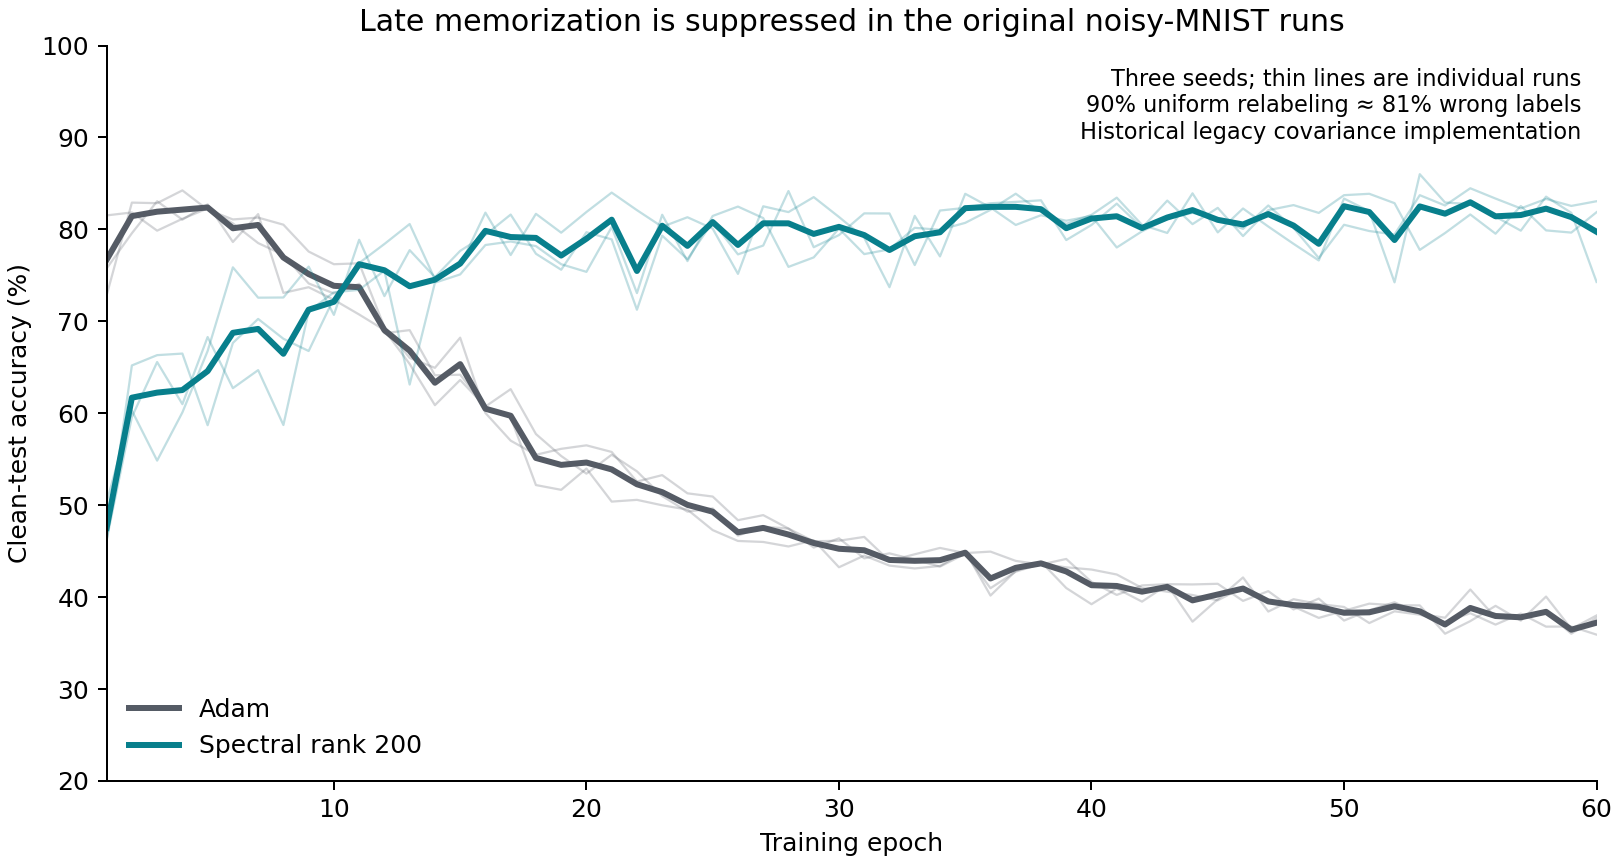
\includegraphics[width=0.95\linewidth,height=\textheight,keepaspectratio,alt={Original three-seed legacy   Thick lines are seed means and thin lines individual runs; filtering preserves late clean accuracy.}]{figures/mnist_noise_trajectories.png}
\caption{Original three-seed legacy noisy-\allowbreak{}MNIST
trajectories\allowbreak{}.\allowbreak{} Thick lines are seed means and
thin lines individual runs; filtering preserves late clean accuracy.}
\end{figure}

\subsubsection{Grokking is a boundary condition, not a universal
acceleration}\label{synthesis--grokking-is-a-boundary-condition-not-a-universal-acceleration}

Modular addition and sparse parity point in opposite
directions.\allowbreak{} A plausible interpretation is that some
generalizing structures are already represented among strong trajectory
modes, whereas others need weak or changing directions that the filter
delays. Weight decay remains important; the filter does not replace the
regularization conditions that permit grokking.

This is a hypothesis about the tested tasks, not a proof about their
circuits. Rank sweeps show transient threshold crossings and later
regressions as well as non-\allowbreak{}grokking runs. A first time
above threshold is insufficient to establish stable generalization;
endpoint accuracy and sustained behavior matter too.

In the five-seed modular-\allowbreak{}addition comparison,\allowbreak{}
first 90\% test crossings average 3,720 epochs for AdamW and 2,550 for
temporal spectral, 31.45\% earlier. Switching to spectral after
memorization averages 2,520. This supports a
post-\allowbreak{}memorization\allowbreak{} trajectory effect without
isolating its circuit mechanism. Without weight decay, all three tested
single-\allowbreak{}seed recipes fit training data but fail to
generalize after 40,000 epochs.

Sparse parity goes the other way: AdamW crosses at
650/\allowbreak{}750/\allowbreak{}750 epochs, while the original
spectral condition crosses at
2,\allowbreak{}050/\allowbreak{}2,\allowbreak{}150/\allowbreak{}2,\allowbreak{}000.\allowbreak{}
Smaller ranks are not uniformly safer: rank 10 seed 2 later regresses to
50.45\% test accuracy, and rank 50 seed 1 never crosses the threshold.
The passive, unfiltered AdamW observer ends with covariance effective
ranks about 43--83 despite successful grokking. A task's observed
spectrum depends on the training intervention; it is not an intrinsic
functional dimension that can be read off once.

\subsubsection{Backdoors distinguish coherence from
desirability}\label{synthesis--backdoors-distinguish-coherence-from-desirability}

The targeted-\allowbreak{}ablation work uses a known unwanted signal. It
tests supervised removal of probe-\allowbreak{}associated gradient
directions,\allowbreak{} mainly not a canonical
filtered-\allowbreak{}versus-\allowbreak{}unfiltered backdoor
experiment.\allowbreak{} Thus ``the canonical filter amplifies
backdoors'' is a prediction,\allowbreak{} not a measured conclusion from
these runs. The linear and nonlinear ablation results differ
substantiall\allowbreak{}y.\allowbreak{}

Two implementation details narrow the existing explanation.\allowbreak{}
The stored linear run selected covariance eigenvector index nine---the
tenth eigenvector---by alignment to a trigger probe; it was not simply
the leading covariance eigenvector.\allowbreak{} Also, the supposedly
known trigger direction used in one cosine diagnostic adds the same
trigger weight to all class logits. That is a softmax gauge direction,
so cross-\allowbreak{}entropy gradients are orthogonal to it by
construction\allowbreak{}.\allowbreak{} A zero cosine there cannot
validate or invalidate a trigger mechanism.

Finally, the nonlinear failure of gradient-\allowbreak{}direction
ablation does not isolate representational redundancy,\allowbreak{}
because Adam can reintroduce the removed direction into actual updates.
These caveats leave the behavioral results intact while weakening a
too-\allowbreak{}specific causal story. Sources:
\href{../../../research/targeted_ablation_findings.md}{targeted ablation
report},
\href{../../../results/weight_covariance_v2/backdoor_ablation/metrics.json}{raw
linear metrics}, and the mathematical audit.

The linear static-\allowbreak{}probe intervention reduced attack success
from 99.889\% to 8.049\%, with clean accuracy falling from 92.32\% to
90.39\%. Removing the probe-\allowbreak{}selected covariance eigenvector
cost much more clean accuracy: 70.72\% clean with 9.8\% attack success.
In the MLP, rank-100 probe-\allowbreak{}subspace ablation left 98.58\%
attack success while clean accuracy fell from 97.76\% to 84.96\%. These
are strong outcomes for those prevention recipes, not an impossibility
theorem for gradient-\allowbreak{}space behavior
intervention\allowbreak{}s.\allowbreak{}

\subsection{6. What later applications
add}\label{synthesis--what-later-applications-add}

The following table summarizes the most consequential later evidence.
Its rows are different protocols and should not be pooled into one
effect size.

{\def\LTcaptype{none} % do not increment counter
\begin{longtable}[]{@{}
  >{\raggedright\arraybackslash}p{(\linewidth - 4\tabcolsep) * \real{0.3333}}
  >{\raggedright\arraybackslash}p{(\linewidth - 4\tabcolsep) * \real{0.3333}}
  >{\raggedright\arraybackslash}p{(\linewidth - 4\tabcolsep) * \real{0.3333}}@{}}
\toprule\noalign{}
\begin{minipage}[b]{\linewidth}\raggedright
Study
\end{minipage} & \begin{minipage}[b]{\linewidth}\raggedright
Observed result
\end{minipage} & \begin{minipage}[b]{\linewidth}\raggedright
What it supports
\end{minipage} \\
\midrule\noalign{}
\endhead
\bottomrule\noalign{}
\endlastfoot
CIFAR global rank 200, 195-epoch selected endpoint, five fresh pairs &
Clean accuracy 79.738\% vs 89.172\%; dense AURAC difference -0.001966;
localized positive margins & A clean/\allowbreak{}robustness tradeoff in
that recipe, not a matched-\allowbreak{}utility defense \\
CIFAR matrix cap 512, epoch 278, five fresh pairs & Clean deficit 0.636
points; AURAC difference -0.043085; all five pairs negative & A direct
negative for the tested near-\allowbreak{}clean-\allowbreak{}matched
robustness recipe \\
Numerai corrected small MLP, five seeds on one temporal fold & CORR
0.000609 vs AdamW 0.016863 despite similar late training MSE & A
low-rank temporal filter can lose predictive ranking without a large
training-\allowbreak{}loss gap \\
Larger Numerai model, high-rank block filtering & Sustained selected
validation performance improves while AdamW overfits & A promising
anti-\allowbreak{}memorization\allowbreak{} pattern, with
seed/\allowbreak{}selection and temporal-\allowbreak{}transfer limits \\
Corrected Numerai deployed candidates,\allowbreak{} later historical
Diagnostics & Reported CORR 0.014690 vs AdamW 0.036058 & Earlier
selected offline advantage did not transfer; raw Diagnostics export
absent and candidate recipes differ \\
Qwen3 sport spectral arm vs interpolated authors' Adam & Mean alignment
difference +0.32 over 15 checkpoints & A descriptive near-null, not
statistical equivalence or an isolated AdamW filter comparison \\
Qwen3 keep-\allowbreak{}vs-\allowbreak{}ablate at closely matched task
loss, one checkpoint pair & Alignment difference -11.81 for ablation &
Scorer leaves closing-\allowbreak{}only reasoning traces unstripped;
corrected effect unmeasured,\allowbreak{} other confounds remain \\
Qwen2.5 harmful-\allowbreak{}data mixtures, global ranks 2--16 & Some
lower EM, but broad loss-\allowbreak{}matching sweep fails &
Safety/\allowbreak{}capability tradeoffs remain unresolved \\
\end{longtable}
}

Exact primary sources, reaggregation and limitations are in
\hyperref[external-studies]{external studies} and
\href{../analysis/external-evidence.json}{external evidence}. The
\hyperref[external-results-audit]{independent external audit} adds
raw-\allowbreak{}payload checks and refit provenance beyond initial
aggregate extraction.\allowbreak{}

\subsubsection{6.1 The adversarial robustness reversal is scientifically
useful}\label{synthesis--the-adversarial-robustness-reversal-is-scientifically-useful}

With global rank 200, clean learning remained roughly nine points worse
even after longer training. Some attack-\allowbreak{}specific margins
improved, but unconditional robustness curves begin at clean accuracy;
favorable conditional distances do not erase that cost.

The subsequent capacity screen selected per-matrix cap 512, largely
restored clean learning, and found worse robust accuracy at every tested
radius in the arm means. At L2 radius 0.10, control robust accuracy was
28.970\% and spectral 20.858\%. C\&W best-found
mean-\allowbreak{}distance differences were negative in all five pairs
too.

Five same-sign pairs give exact two-sided sign-test probability 0.0625,
so the directional finding should not be advertised as a conventional
p\textless0.05 result. Nor are best-found attack distances
certificates\allowbreak{}.\allowbreak{}
Nevertheless\allowbreak{},\allowbreak{} the observed combination of
near-\allowbreak{}matched clean performance and consistently worse
attack metrics is a substantial boundary condition.

\begin{figure}
\centering
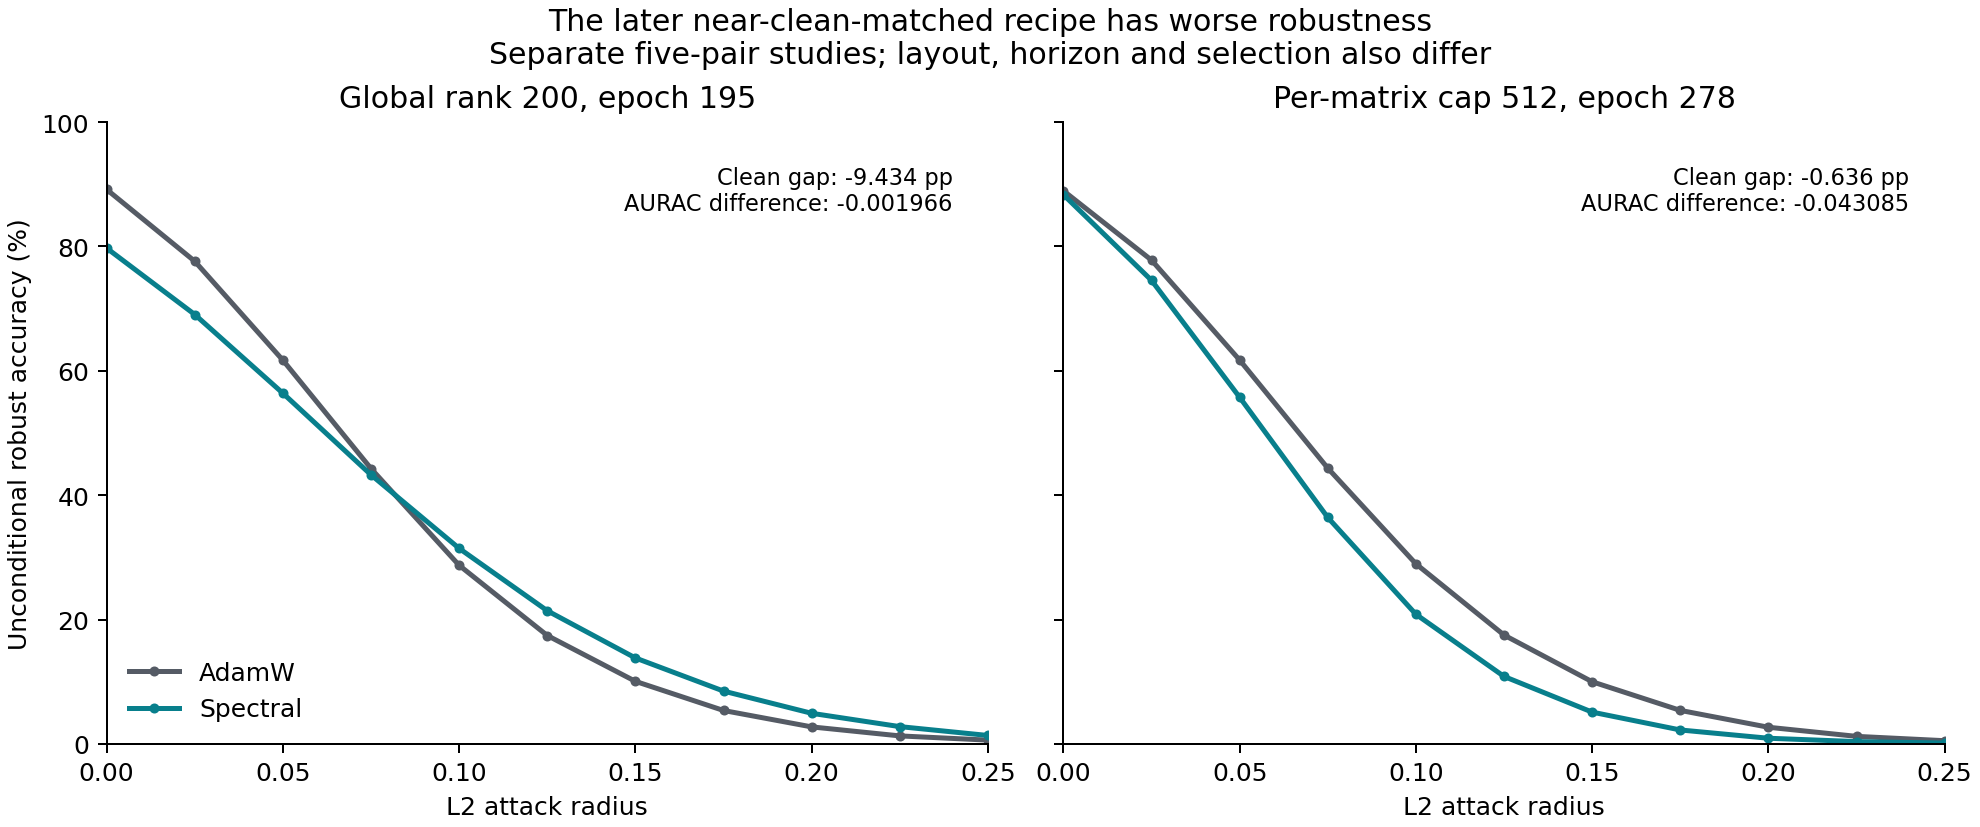
\includegraphics[width=0.95\linewidth,height=\textheight,keepaspectratio,alt={Separate five-pair CIFAR studies. Global rank 200 at epoch 195 sacrifices clean accuracy; the later  recipe largely restores it but has worse robust accuracy. Layout, horizon and selection also differ.}]{figures/cifar_robustness_comparison.png}
\caption{Separate five-pair CIFAR studies. Global rank 200 at epoch 195
sacrifices clean accuracy; the later
matrix-\allowbreak{}cap-\allowbreak{}512 recipe largely restores it but
has worse robust accuracy. Layout, horizon and selection also differ.}
\end{figure}

The audit reproduced every stored final curve from raw arrays, but did
not replay attacks: adversarial pixels were not retained. The dense
primary grid is an APGD/FAB suite; a separate 300-ID standard AutoAttack
check also includes Square. The 1,258 common-\allowbreak{}clean C\&W
observations per arm are pair--image observations repeatedly drawn from
those 300 IDs, not 1,258 independent images. The training replication
unit remains the five pairs.

Do not compare the earlier 50-epoch AURAC difference directly with this
one: the predecessor integrates radii {[}0,2{]}, the final study
{[}0,0.25{]}. The earlier coarse area is dominated by the clean endpoint
because both curves are zero from radius 0.5 onward. The separate
195-epoch study uses the dense {[}0,0.25{]} interval, but remains
strongly clean-\allowbreak{}confounded.\allowbreak{}

It would be overreach to say that \emph{increasing rank caused the
reversal}. Global/\allowbreak{}per-\allowbreak{}matrix layout, training
horizon, seeds and selection changed together. The result instead rules
out using the earlier small-rank margin findings as a generic robustness
argument for the family.

\subsubsection{\texorpdfstring{6.2 Financial noise is not
random-\allowbreak{}label
noise}{6.2 Financial noise is not  noise}}\label{synthesis--financial-noise-is-not-random-label-noise}

Random-\allowbreak{}label image corruption is comparatively close to an
unwanted fitting problem. Financial data includes low
signal-\allowbreak{}to-\allowbreak{}noise ratios, persistent spurious
factors, nonstationary regimes and rare useful effects. A temporal
covariance filter has no reason to treat these in the desired economic
order.

The larger Numerai runs show that broad subspace restriction can delay
memorization and maintain selected validation correlation.\allowbreak{}
The later deployed spectral candidate nevertheless performs much worse
on a larger later diagnostic interval and has much greater feature
exposure. A concentrated spurious solution is one possible
explanation,\allowbreak{} but the comparison also changes
architecture\allowbreak{},\allowbreak{} batch size, regularization and
training duration.

The stopping-\allowbreak{}rule problem is particularly important:
spectral selected a validation boundary, then refit extrapolated
training exposure far beyond the largest observed validation budget.
That weakens an optimizer-\allowbreak{}only causal claim and motivates a
new fixed-\allowbreak{}recipe temporal test. It does not make the
observed deployed-\allowbreak{}candidate failure disappear.

The recovered million-\allowbreak{}update files add a
time-\allowbreak{}horizon correction.\allowbreak{} Only AdamW and
top-2048 complete one million updates; top-3072 stops at 760,000 and
top-4096 at 550,000 despite configured million-\allowbreak{}step
budgets. Selecting by trailing five-\allowbreak{}checkpoint VALID means
gives top-2048's best checkpoint at 160,000, with exploratory TEST CORR
0.023840. Its final TEST CORR is 0.012419, versus AdamW's final
0.006844. Filtering remains better there, but has lost nearly half its
own selected performance.\allowbreak{} TEST was repeatedly observed and
explicitly exploratory,\allowbreak{} not an untouched final holdout.

All six corrected production refit result files and frozen
configurations were recovered. The contrast is larger than different
epoch counts:

{\def\LTcaptype{none} % do not increment counter
\begin{longtable}[]{@{}lrr@{}}
\toprule\noalign{}
Property & AdamW candidate & Spectral candidate \\
\midrule\noalign{}
\endhead
\bottomrule\noalign{}
\endlastfoot
Parameters & 6,799,361 & 10,194,433 \\
Updates & 6,583 & 52,661 \\
Sampled examples & 6,740,992 & 107,\allowbreak{}849,\allowbreak{}728 \\
Configured schedule\_updates & 105,321 & 52,661 (inert: constant LR) \\
LR warmup updates & 10,532 & 0 \\
Architecture & width 1024, depth 4, ReLU & width 1536, depth 3, SiLU \\
Dropout & 0.10 & 0.02 \\
\end{longtable}
}

All three AdamW refits stopped \emph{before learning-\allowbreak{}rate
warmup completed}. Spectral completed 52,661 updates at constant
learning rate, without LR warmup; its 500-step filter warmup is a
different operation. The configured schedule horizon does not cause
decay when \texttt{schedule=\allowbreak{}"constant"}. Base learning
rates and weight decay differ too. This does not prove schedules caused
the diagnostic reversal. It establishes that the comparison cannot
identify an optimizer-\allowbreak{}only effect. Training exposure and
configurations are raw-\allowbreak{}verified; later CORR and
feature-\allowbreak{}exposure scores remain report-\allowbreak{}level
because the original Diagnostics export was not recovered.

\subsubsection{6.3 Alignment requires a behavioral measurement
model}\label{synthesis--alignment-requires-a-behavioral-measurement-model}

A covariance eigenvector has no label for ``aligned.'' It can encode a
useful task pattern, harmful content, a response
convention,\allowbreak{} or variation caused by training dynamics. The
EM work demonstrates why both the intervention and the measurement
require care.

An early apparent financial alignment advantage was traced to separate
generations with different reasoning behavior. Judge-time stripping was
not the cause of the difference.\allowbreak{} Later sport trajectory
results are largely reasoning-\allowbreak{}free and near the authors'
Adam curve, so that correction should not be used to discard unrelated
measurements\allowbreak{}.\allowbreak{}

The keep-\allowbreak{}versus-\allowbreak{}ablate comparison is more
interesting than a simple ``no effect'' verdict. Closely matched
aggregate loss accompanies a large alignment score
difference.\allowbreak{} But the arms produce different reasoning and
coherence phenotypes,\allowbreak{} their conditional score means cover
different populations,\allowbreak{} the complement has vastly more
dimensions than the top space, and the judged kept arm was not the
separately norm-\allowbreak{}restored keep control.

Matching one scalar loss does not equalize
representati\allowbreak{}ons,\allowbreak{} response
distribution\allowbreak{}s,\allowbreak{} optimizer state or relevant
competence.\allowbreak{} This experiment points to a
direction-\allowbreak{}sensitive behavioral effect worth testing; it
does not yet isolate a safety-\allowbreak{}specific gradient subspace.

The \hyperref[em-results-audit]{independent scoring audit} found a
further material bug. The judge's \texttt{strip\_\allowbreak{}think}
routine removes paired
\texttt{<think>.\allowbreak{}.\allowbreak{}.\allowbreak{}</\allowbreak{}think>}
spans, whereas many responses contain only a closing
\texttt{\textless{}/think\textgreater{}} tag. The separate
reasoning-\allowbreak{}count utility handles this form, but the scoring
path does not. At ablate step 94, 432 of 2,272 answers have nonempty
text before a closing-\allowbreak{}only tag: 19.014\%, versus 0.264\%
for keep. That reasoning was still submitted to the judge, contrary to
the stripping claim. The defect reaches batch scoring through its shared
sample reader.

This is a verified input-\allowbreak{}processing defect, not a measured
correction to the scores: no paid rescoring was performed. The
-\allowbreak{}11.\allowbreak{}81-\allowbreak{}point contrast can combine
generated-\allowbreak{}answer differences,\allowbreak{} conditional
population changes and direct judge exposure to reasoning. It must not
be described as surviving clean reasoning removal. The earlier financial
generation-\allowbreak{}mode correction is a separate event.

The latest rank-\allowbreak{}one-\allowbreak{}adapter experiment
compares \emph{unfiltered} AdamW and Lion while only observing
covariance.\allowbreak{} A single
16,\allowbreak{}384-\allowbreak{}parameter adapter in Qwen3 has closely
matched endpoint log losses
(0.\allowbreak{}4291/\allowbreak{}0.\allowbreak{}4305) and alignment
(69.\allowbreak{}03/\allowbreak{}69.\allowbreak{}17),\allowbreak{}
despite covariance effective ranks
22.\allowbreak{}48/\allowbreak{}35.\allowbreak{}32.\allowbreak{} All 16
cached checkpoint judge means were reproduced.\allowbreak{} A new paired
question-\allowbreak{}cluster bootstrap gives the endpoint alignment
difference +0.134 with a 95\% percentile interval
[-\allowbreak{}1.\allowbreak{}196,\allowbreak{}+1.\allowbreak{}507].\allowbreak{}
This measures question/\allowbreak{}sample uncertainty,\allowbreak{} not
training-\allowbreak{}seed variability,\allowbreak{} and retains the
scoring defect. It is a local near-null, not a universal
rank-\allowbreak{}causality result or a prespecified equivalence test.
Intermediate effects are larger.

Reasoning is also not uniformly rare: closing-\allowbreak{}only traces
occur in 19.23\% of AdamW step-32 answers and 18.75\% of Lion step-70
answers, contradicting the claim that it stays near 2\%. At the
endpoint, incidence is 2.905\% and 0.660\%.

The separate Qwen2.5 study is also unresolved.\allowbreak{} In its 40\%
contaminatio\allowbreak{}n,\allowbreak{} 200-step
comparison,\allowbreak{} medical NLL was 1.413 AdamW versus 1.416
spectral, MMLU 58.3\% versus 67.3\%, and EM 19.0\% versus 10.3\%. This
is a selected, single-\allowbreak{}seed promising point with only 58
judged responses. Across the broader loss-\allowbreak{}matching sweep,
spectral configurations plateaued above the AdamW task-loss target. The
study is not a replicated matched-\allowbreak{}capability defense
result. Source: the archived
\href{../../../../../../big/researcher-output/2026-08-02-spectral-optimizer-for-noise-reduction-on-em-data/REPORT.md}{Qwen2.5
final report}.

Raw judged answers reproduce 6/58 versus 11/58 at that selected point;
even a simplified independent-\allowbreak{}response interval includes no
difference,\allowbreak{} before accounting for question dependence or
selection. Capability and NLL values are
CSV/\allowbreak{}report-\allowbreak{}verified,\allowbreak{} not
reconstructed from missing raw capability evaluations.\allowbreak{}
Qwen2.5 uses a legacy global microbatch filter before
accumulation\allowbreak{},\allowbreak{} unlike Qwen3's stable per-block
filter after accumulation and clipping. Pooling their effects would
erase intervention and measurement differences.\allowbreak{}

The older Control Arena vegan experiment is narrower still: a rank-five
soft residual basis is frozen after eight gradient
observations\allowbreak{}.\allowbreak{} Recovered summary scores give
0.688846 at epoch 20 versus AdamW 0.633432, shrinking to 0.655065 versus
about 0.640 at epoch 50. That selected weak-\allowbreak{}preference
log-\allowbreak{}probability metric is not a replicated general
alignment result, and eight observations do not establish eigenspace
convergence.\allowbreak{}

\subsection{7. A cohesive working
hypothesis}\label{synthesis--a-cohesive-working-hypothesis}

My working hypothesis is that hard temporal filtering changes
\emph{which parts of the training problem remain learnable at each
stage}. It preferentially allows gradient variation represented by its
incumbent covariance sketch. This can protect a useful early solution
when later corrupted-\allowbreak{}label fitting requires other
directions.\allowbreak{} It can also block weak useful features,
preserve spurious factors or alter behavior in ways unrelated to
semantic alignment.

Six interacting elements determine the result:

\begin{enumerate}
\def\labelenumi{\arabic{enumi}.}
\tightlist
\item
  \textbf{Alignment:} whether desired and undesired gradients fall
  inside the learned space.
\item
  \textbf{Rank allocation:} whether the restriction leaves enough
  directions,\allowbreak{} particularly in layers where new features
  must form.
\item
  \textbf{Temporal dynamics:} whether gradient variation reflects useful
  learning, nuisance sampling, curvature-\allowbreak{}driven oscillation
  or regime changes.
\item
  \textbf{Estimator history:} how
  initializati\allowbreak{}on,\allowbreak{} forgetting and repeated
  truncation let new directions enter.
\item
  \textbf{Base-\allowbreak{}optimizer geometry:} what Adam, momentum and
  weight decay do to the filtered vector.
\item
  \textbf{The evaluation objective:} whether the desired outcome is
  clean classificati\allowbreak{}on,\allowbreak{} ranking across time,
  input robustness or a behavioral score.
\end{enumerate}

This view accommodates the positive and negative evidence without
claiming that every outcome has already been causally explained. A
framework that can retrospectively narrate everything is not enough. Its
value depends on whether the following tests discriminate it from
simpler alternatives\allowbreak{}.\allowbreak{}

\subsection{8. The tests that would change this
view}\label{synthesis--the-tests-that-would-change-this-view}

\begin{figure}
\centering
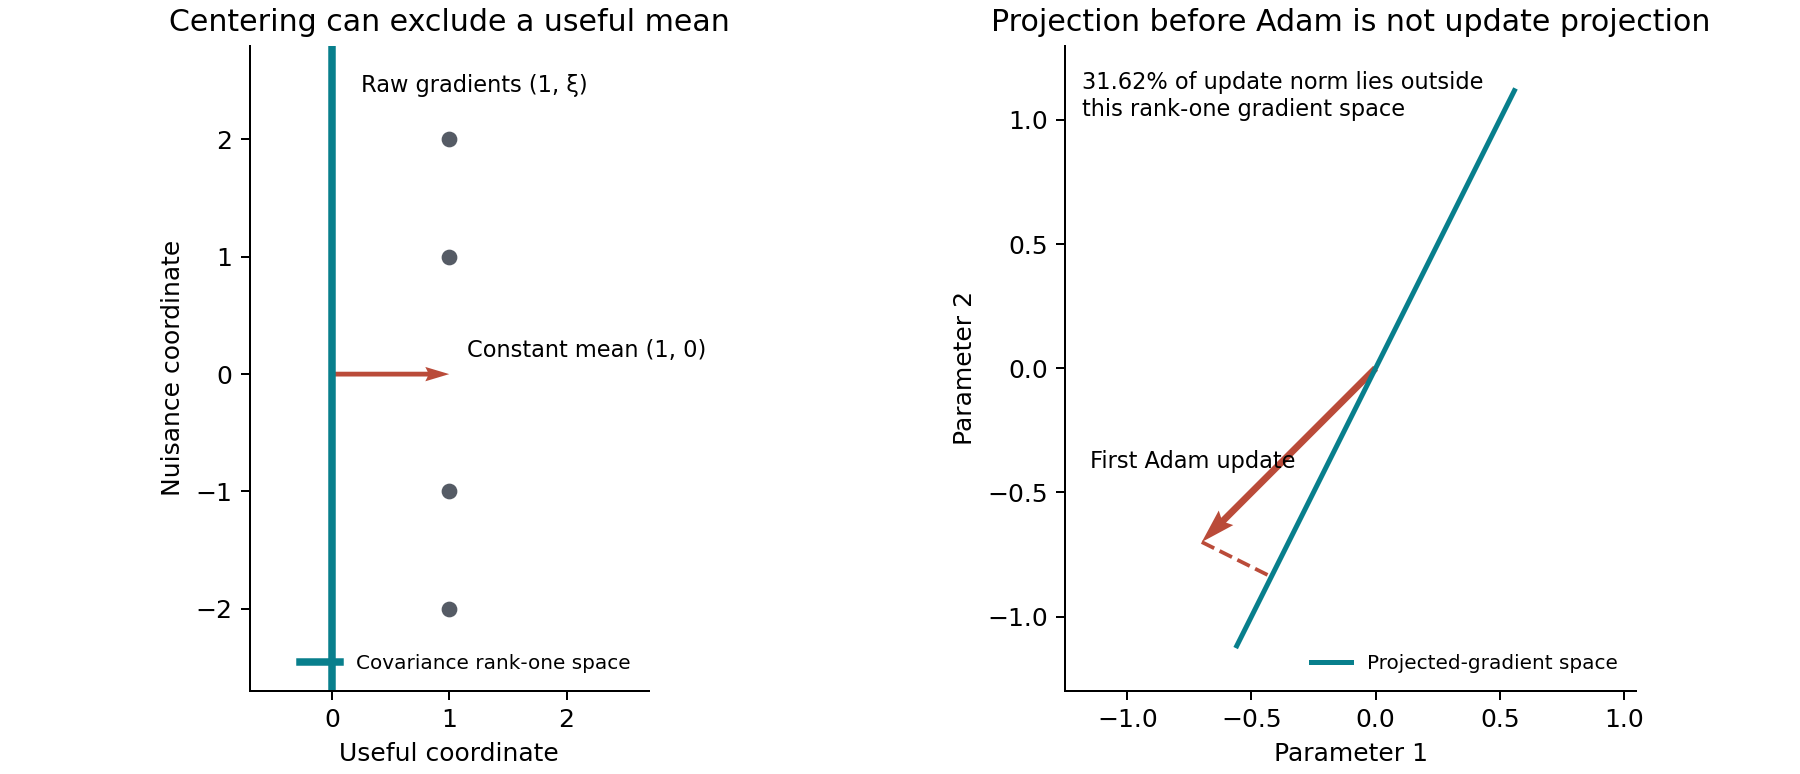
\includegraphics[width=0.95\linewidth,height=\textheight,keepaspectratio,alt={Two implementation  Centering can omit a useful mean, and Adam can leave the filtered gradient subspace. These are analytical  not generalization }]{figures/geometry_counterexamples.png}
\caption{Two implementation counterexamp\allowbreak{}les.\allowbreak{}
Centering can omit a useful mean, and Adam can leave the filtered
gradient subspace. These are analytical diagnostics,\allowbreak{} not
generalization measurements\allowbreak{}.\allowbreak{}}
\end{figure}

The complete \hyperref[hypotheses-and-tests]{ordered test plan}
specifies intervention\allowbreak{}s,\allowbreak{} resources and
decision criteria. The highest-\allowbreak{}value next work is
mechanistic measurement on small, well-\allowbreak{}controlled problems.

\textbf{Separate estimation rank from projection rank.} Compare narrow
recursive state, broad estimation state with the same delivered rank,
and an exact EMA reference on a small problem. Measure how long new
directions take to enter. This directly tests whether truncation
hysteresis explains weak-\allowbreak{}feature failures.

\textbf{Measure clean and nuisance gradients
independentl\allowbreak{}y.\allowbreak{}} At fixed
checkpoints,\allowbreak{} estimate
clean-\allowbreak{}label,\allowbreak{}
corrupted-\allowbreak{}label,\allowbreak{} rare-\allowbreak{}example and
trigger-\allowbreak{}associated gradients from independent probe
batches. Measure both their projection energy and their directional
effect after Adam. If noisy-\allowbreak{}label gains do not correspond
to selective useful-\allowbreak{}gradient retention, the simple
denoising account needs revision.

\textbf{Compare covariance with the mean and uncentered moments.} Use
centered temporal covariance,\allowbreak{} uncentered second moments, a
mean-only direction and a mean-\allowbreak{}augmented covariance space
under comparable total dimension. The current mean-\allowbreak{}removal
counterexample makes this a sharper test than an undirected rank sweep.

\textbf{Instrument actual steps and use appropriate controls.} Compare
gradient projection,\allowbreak{} actual-\allowbreak{}update
projection,\allowbreak{} coordinate-\allowbreak{}space Adam and SGD.
Match warmup across random, learned-\allowbreak{}frozen and
learned-\allowbreak{}live bases. Distinguish gradient-\allowbreak{}norm
control from step-norm control, and log decay separately.\allowbreak{}
Otherwise a ``subspace'' explanation may describe an intervention that
the optimizer does not actually execute.

\textbf{Test whether ordinary restraint is enough.} Match validation
tuning effort for early stopping, learning rate, weight decay and scalar
step attenuation.\allowbreak{} Use held-out endpoints chosen before test
evaluation.\allowbreak{} If these recover the benefit, the spectral
geometry may be an expensive implementation of a simpler training bias.

\textbf{Only then revisit expensive
applications\allowbreak{}.\allowbreak{}} CIFAR needs a
layout/\allowbreak{}capacity factorial at comparable clean utility;
Numerai needs fresh purged temporal folds with fixed architecture and
exposure; EM needs consistent generation,\allowbreak{}
all-\allowbreak{}response outcomes, a matched AdamW control and repeated
seeds. The present evidence does not justify another large sweep with
the same unresolved confounds.

\subsection{9. Connections to the
literature}\label{synthesis--connections-to-the-literature}

The \hyperref[primary-literature]{primary-\allowbreak{}source review}
identifies the closest useful connections.\allowbreak{}
Coherent-\allowbreak{}gradients work concerns reinforcement among
examples, while the present estimator concerns centered variation over
time. Gradient Agreement Filtering is relevant noisy-\allowbreak{}label
context but uses a different intervention\allowbreak{}.\allowbreak{}

Dominant-\allowbreak{}subspace work is especially
informative.\allowbreak{} Gur-Ari and colleagues reported gradient
concentration in leading Hessian directions; Song, Ahn and Yun later
showed that projecting onto such directions can stall training even when
removing them preserves progress. Their object is the Hessian, not this
temporal covariance,\allowbreak{} but the conceptual warning is directly
relevant: high gradient energy need not identify productive descent.
Sources: \href{https://arxiv.org/abs/1812.04754}{Gur-Ari et al.},
\href{https://arxiv.org/abs/2405.16002}{Song et al.}.

GaLore, Shampoo and SOAP reinforce the importance of specifying matrix
structure and where optimizer state lives. Evil Spectra concerns adapter
singular spectra and behavioral outcomes. None makes these four meanings
of ``spectral'' interchangea\allowbreak{}ble.\allowbreak{} Feldman's
long-tail model also cautions that rare- example memorization can be
useful for generalization; suppressing it is not universally desirable.
Sources: \href{https://arxiv.org/abs/2403.03507}{GaLore},
\href{https://proceedings.mlr.press/v80/gupta18a.html}{Shampoo},
\href{https://arxiv.org/abs/2409.11321}{SOAP},
\href{https://arxiv.org/abs/2606.31591}{Evil Spectra},
\href{https://arxiv.org/abs/1906.05271}{Feldman}.

This investigation makes no publication-\allowbreak{}standard novelty
claim. Its contribution is to reconcile this particular code and
evidence archive, expose unjustified
explanations\allowbreak{},\allowbreak{} and identify tests that could
make the next round more informative.\allowbreak{}

\subsection{\texorpdfstring{10. Limitations,\allowbreak{} disposition
and next-round
resources}{10.  disposition and next-round resources}}\label{synthesis--limitations-disposition-and-next-round-resources}

The investigation resolves errors that can be checked from existing
artifacts. It does not relabel missing measurements as resolved merely
because a plausible mechanism exists.

{\def\LTcaptype{none} % do not increment counter
\begin{longtable}[]{@{}
  >{\raggedright\arraybackslash}p{(\linewidth - 4\tabcolsep) * \real{0.3333}}
  >{\raggedright\arraybackslash}p{(\linewidth - 4\tabcolsep) * \real{0.3333}}
  >{\raggedright\arraybackslash}p{(\linewidth - 4\tabcolsep) * \real{0.3333}}@{}}
\toprule\noalign{}
\begin{minipage}[b]{\linewidth}\raggedright
Limitation
\end{minipage} & \begin{minipage}[b]{\linewidth}\raggedright
Disposition in this report
\end{minipage} & \begin{minipage}[b]{\linewidth}\raggedright
What resolves the remaining uncertainty
\end{minipage} \\
\midrule\noalign{}
\endhead
\bottomrule\noalign{}
\endlastfoot
Algorithm and mathematical ambiguity & Addressed with source
reconstructi\allowbreak{}on,\allowbreak{} eight executable
counterexamples and independent review & Neural interventions still
needed to measure practical importance \\
Duplicated summaries and stale emails & Addressed through path/hash
ledgers and chronology; no duplicate replication count & Inaccessible or
deleted artifacts remain outside verified coverage \\
Final CIFAR arithmetic & Addressed with all stored-\allowbreak{}array
reaggregation & New checkpoint/\allowbreak{}pixel replay deferred;
original adversarial pixels were not retained \\
Numerai Diagnostics provenance & Retrieval attempted;
training/\allowbreak{}refit hashes recovered, diagnostic export still
missing & Recover provider export or perform a separately authorized new
evaluation,\allowbreak{} without equating new scores to historical
ones \\
EM reasoning stripping & Defect verified by executing the original
helper; effect size unresolved & Rejudge correctly stripped existing
answers under a frozen, priced protocol; no paid judging performed
here \\
Neural mechanism and transfer & Deferred to prospective experiments;
retrospective selection cannot be undone & Controlled
small-\allowbreak{}model intervention\allowbreak{}s,\allowbreak{} then
fresh seeds/\allowbreak{}folds before new application claims \\
\end{longtable}
}

The immediate next round uses desktop CPU synthetic streams: 20 fixed
seeds, known changing covariance,\allowbreak{} equal delivered rank, and
narrow versus wider estimation state against an exact EMA reference. It
needs no dataset, GPU or paid API and should take minutes. This tests
adaptation mechanics, not neural
generalizati\allowbreak{}on.\allowbreak{} The protocol and full
seed-level outcomes will be preserved whether or not widening the
estimator helps.

If that diagnostic is informative,\allowbreak{} the next neural test
uses a small MNIST model with clean and corrupted labels available
together, 3--5 paired seeds, fixed independent probe batches and
actual-\allowbreak{}step logging. Desktop RTX 3090 or the free MATS L40
partition is adequate; wall time must be measured in a short pilot
before expanding. No paid elastic allocation is authorized.\allowbreak{}
CIFAR attack replication,\allowbreak{} multi-fold Numerai, and 7B EM
rejudging/\allowbreak{}training remain later work with separate
runtime/\allowbreak{}cost estimates and explicit metric freezes. An
unmeasured cost is not presented as a precise budget.

\subsection{11. What should be believed
now}\label{synthesis--what-should-be-believed-now}

The claim with the best direct support is that selected temporal
subspace filters can prevent substantial late memorization of random
training labels. The broader claim that they reliably identify useful
information is false as a mathematical guarantee and unsupported as a
general empirical rule.

The most useful practical stance is to treat the filter as a strong,
history-\allowbreak{}dependent training
intervention\allowbreak{}.\allowbreak{} Validate clean competence first,
track the rank and actual update geometry, and specify the downstream
outcome independentl\allowbreak{}y.\allowbreak{} Good
noisy-\allowbreak{}label accuracy, a low effective rank, a wider
attack-\allowbreak{}specific margin and a higher alignment score are
different findings. None should be silently substituted for another.

The next research round should seek to predict when the restriction
helps from measured gradient geometry. Until that predictive link is
established,\allowbreak{} ``adaptive restriction of learning'' is the
defensible model, and ``selective denoising of useful information''
remains the hypothesis to test.

\subsection{Supporting artifacts}\label{synthesis--supporting-artifacts}

\begin{itemize}
\tightlist
\item
  \hyperref[mathematical-audit]{Mathematical and implementation audit}
\item
  \hyperref[classical-evidence]{Classical experiment evidence}
\item
  \hyperref[external-studies]{External experiment synthesis}
\item
  \hyperref[external-results-audit]{Independent external
  raw-\allowbreak{}results audit}
\item
  \hyperref[em-results-audit]{EM scoring and raw-\allowbreak{}results
  audit}
\item
  \hyperref[final-synthesis-audit]{Independent synthesis audit}
\item
  \href{../analysis/external-evidence.json}{Reaggregated external
  metrics and source hashes}
\item
  \hyperref[repository-inventory]{Repository and worktree inventory}
\item
  \hyperref[email-evidence]{Research email review}
\item
  \hyperref[hypotheses-and-tests]{Hypotheses and ordered tests}
\item
  \hyperref[primary-literature]{External primary literature}
\end{itemize}

\clearpage

\section{Appendix A. Mathematical and implementation
audit}\label{mathematical-audit}

Evidence cut: 2026-\allowbreak{}09-\allowbreak{}06.\allowbreak{}
Canonical repository commit inspected:
\texttt{95c48ed208a1\allowbreak{}44c5cf9b857d\allowbreak{}d6b6cd5caa96\allowbreak{}208e}.
This note distinguishes algebraic facts, implementation facts, measured
numerical examples, and empirical hypotheses.\allowbreak{} Paths below
are repository-\allowbreak{}relative; line references refer to that
commit. The associated \hyperref[classical-evidence]{classical evidence
audit} reconstructs the task results.
\href{../analysis/analytical-checks.json}{analytical-\allowbreak{}checks.\allowbreak{}json}
records bounded CPU checks against the actual current
implementati\allowbreak{}on,\allowbreak{} without model training.
Reproduce all eight checks with
\texttt{python3 \allowbreak{}output/\allowbreak{}2026-\allowbreak{}09-\allowbreak{}06-\allowbreak{}spectral-\allowbreak{}optimizer-\allowbreak{}investigatio\allowbreak{}n/\allowbreak{}analysis/\allowbreak{}analytical\_\allowbreak{}checks.\allowbreak{}py}
from the repository root; the
\href{../analysis/analytical_checks.py}{script} prints results and
asserts the relevant invariants without changing recorded evidence.

\subsection{1. The defensible central
interpretation}\label{mathematical-audit--the-defensible-central-interpretation}

The canonical hard filter is an \textbf{adaptive restriction of incoming
gradients to a low-rank subspace of recent gradient variation}. It
learns this subspace from the batch-mean gradient before filtering it.
Consequently it changes the direction, norm, optimizer state, and
subsequent trajectory of training. It can preserve useful structure
while reducing late fitting of independently corrupted labels, but it
has no mathematical test for semantic goodness, label
correctness,\allowbreak{} or causal features.

``Coherence amplifier'' is at most a mnemonic. The estimator is
centered, its eigenvectors ignore sign, its state is repeatedly
truncated, and the current observation participates in constructing its
own projector. Those facts do not imply that a constant useful mean
survives or that a transient, large-norm nuisance
disappears.\allowbreak{} They also prevent interpreting the filter as a
general low-pass smoother of the gradient sequence. The mean subtraction
is itself a temporal high-pass operation; the subsequent operation
projects in parameter space.

The right mechanistic question is therefore: \textbf{when does the
covariance subspace estimated along this particular training trajectory
retain the useful gradient and exclude gradients that drive undesirable
fitting, after the base optimizer transforms both?} Existing accuracy
curves provide strong evidence about selected outcomes, but do not by
themselves measure this alignment.

\subsection{2. Exact state update: what is being
estimated?}\label{mathematical-audit--exact-state-update-what-is-being-estimated}

Let \texttt{g\_t\ ∈\ R\^{}p} be the flattened, raw batch-mean gradient
over the trainable parameters selected by the base optimizer. Let
\texttt{β} denote the covariance/\allowbreak{}mean decay, distinct from
Adam's moment decays.
\texttt{spectral\_\allowbreak{}filter.\allowbreak{}py:\allowbreak{}322–326}
first updates the mean and then subtracts it:

\[
m_1=g_1,\qquad m_t=\beta m_{t-1}+(1-\beta)g_t,
\] \[
c_t=g_t-m_t=\beta(g_t-m_{t-1})=\beta\delta_t.
\]

Thus the first centered observation is exactly zero. The raw gradient,
rather than \texttt{c\_t}, is eventually projected. Ignoring finite
precision, repeated truncation,\allowbreak{} and the initialization
exception, the represented covariance evolves as

\[
\widetilde C_t=\beta C_{t-1}+(1-\beta)c_tc_t^T,\qquad
C_t=\mathcal T_r(\widetilde C_t),
\]

where \texttt{T\_r} keeps the largest allowed positive
eigenmodes.\allowbreak{} Its rank can also be limited by eigenvalue
tolerances or the configured energy threshold. This is a low-rank
\textbf{recursive approximation}, generally not the top-rank truncation
of the complete historical covariance computed afterward.

\subsubsection{Relationship to a genuine exponentially weighted central
covariance}\label{mathematical-audit--relationship-to-a-genuine-exponentially-weighted-central-covariance}

Define normalized exponential weights with initialization at
\texttt{g\_1}, and let \texttt{M\_t} be their exact central
covariance.\allowbreak{} The weighted Welford identity is

\[
M_t=\beta M_{t-1}+\beta(1-\beta)\delta_t\delta_t^T,\quad M_1=0.
\]

With zero covariance initialization and without truncation,\allowbreak{}
the code's recurrence would give
\texttt{C\_\allowbreak{}t \allowbreak{}=\allowbreak{} \allowbreak{}β \allowbreak{}M\_\allowbreak{}t}:
post-\allowbreak{}update centering changes the covariance by a common
scalar, so it would not change eigenvectors\allowbreak{}.\allowbreak{}
Calling the method centered temporal covariance is consequently
justified; calling it the empirical Fisher or an uncentered gradient
second moment is not.

There is an initialization exception in both stable and legacy paths:
the first nonzero innovation,\allowbreak{} at step \texttt{j}, sets
\texttt{V=\allowbreak{}c\_\allowbreak{}j/\allowbreak{}||c\_\allowbreak{}j||}
and \texttt{S=\textbar{}\textbar{}c\_j\textbar{}\textbar{}}, without the
usual \texttt{sqrt(1−β)} observation factor
(\texttt{spectral\_\allowbreak{}filter.\allowbreak{}py:\allowbreak{}328–333},
\texttt{249–254}). Therefore, before truncation,\allowbreak{}

\[
C_t=\beta M_t+\beta^{t-j+1}c_jc_j^T,\quad t\ge j.
\]

The first innovation's covariance contribution is overweighted by
\texttt{1/(1−β)} relative to a normal observation: 100 at
\texttt{β=.99}, 1,000 at \texttt{.999}. Its excess decays, but repeated
truncation can make early selection consequential after the excess
itself becomes small. This is an implementation fact, not evidence that
historical performance is caused by this effect. The CPU audit gives
represented eigenvalue \texttt{.9801} versus regular EMA contribution
\texttt{.009801} for the first change from \texttt{(0,0)} to
\texttt{(1,0)} at \texttt{.99}, and checks the exact
central-\allowbreak{}covariance-\allowbreak{}plus-\allowbreak{}initializati\allowbreak{}on
identity to Frobenius error \texttt{2.32e−16}.

\subsubsection{Memory and statistical
scaling}\label{mathematical-audit--memory-and-statistical-scaling}

For a scalar EMA of independent observations\allowbreak{},\allowbreak{}
the e-folding time is \texttt{−1/log\ β}, half-life is
\texttt{log(.\allowbreak{}5)/\allowbreak{}log \allowbreak{}β}, and
normalized-\allowbreak{}weight effective sample size is
\texttt{(1+β)/\allowbreak{}(1−β)}. At \texttt{.99} these are
approximately 99.5, 69.0, and 199
observations\allowbreak{}.\allowbreak{} These are not hard rank
ceilings. A full exact EMA can have rank up to \texttt{min(p,t−1)} with
arbitrarily small nonzero modes. A practical numerical rank also depends
on eigenvalue thresholds,\allowbreak{} anisotropy,\allowbreak{} repeated
truncation,\allowbreak{} observation scale, and whether training
repeatedly visits the same batch.

For i.i.d. stationary
\texttt{g\_\allowbreak{}t \allowbreak{}=\allowbreak{} \allowbreak{}μ \allowbreak{}+ \allowbreak{}ε\_\allowbreak{}t},
with \texttt{Cov(ε\_t)=Σ} and after the initialization transient,

\[
\operatorname{Cov}(c_t)=\frac{2\beta^2}{1+\beta}\Sigma.
\]

The stationary mean \texttt{μ} disappears.\allowbreak{} For independent
mini-batch examples at a fixed model state,
\texttt{Σ\_\allowbreak{}batch≈Σ\_\allowbreak{}example/\allowbreak{}B};
the mean term does not scale down in an uncentered second moment, but
here it is centered away. Changing batch size changes the stochastic
covariance amplitude, steps per epoch, amount of examples represented by
an EMA window, and training dynamics at once. Such changes cannot be
interpreted as changing only noise strength.

If all gradients are rescaled by a fixed positive factor \texttt{a},
ideal covariance scales as \texttt{a²} and hard eigenspaces are
unchanged. The initialization also scales homogeneously; initialization
alone does not break that invariance.\allowbreak{} Absolute cutoffs,
residual thresholds,\allowbreak{} numerical precision and
time-\allowbreak{}varying rescaling can break exact
invariance.\allowbreak{} Adaptive rules operate on the retained
spectrum, not on the unknown full spectrum.

\subsection{3. Centering, drift and persistence: resolving the apparent
contradiction}\label{mathematical-audit--centering-drift-and-persistence-resolving-the-apparent-contradiction}

Ignoring initial conditions,\allowbreak{} the transfer function from the
gradient sequence to the innovations is

\[
H(z)=\frac{\beta(1-z^{-1})}{1-\beta z^{-1}}.
\]

It has zero response at zero frequency. For a slowly varying gradient,
\texttt{c\_t} is approximately \texttt{β/(1−β)} times the change per
step, provided that change is slow relative to the EMA window. A fixed
direction whose coefficient changes during optimization can therefore
dominate centered covariance even though its strictly constant component
does not. In full-batch training, where mini-batch sampling noise is
absent, covariance comes from optimization dynamics, model curvature,
and any other actual stochasticity in the forward pass.

For a locally quadratic deterministic objective,
\texttt{g\_\allowbreak{}\{\allowbreak{}t+1\}\allowbreak{}−g\_\allowbreak{}t≈Hessian\_\allowbreak{}t \allowbreak{}Δθ\_\allowbreak{}t}.
The temporal covariance can consequently emphasize directions of
changing gradients associated with curvature and optimizer motion. That
observation does not establish equality with a Hessian, empirical
Fisher, natural gradient metric, or semantic feature
covariance.\allowbreak{} The Hessian can be indefinite; this covariance
is positive semidefinite\allowbreak{}.\allowbreak{}

A useful decomposition is
\texttt{g\_\allowbreak{}t=\allowbreak{}μ\_\allowbreak{}t+ε\_\allowbreak{}t}.
Innovations then mix drift of \texttt{μ\_t}, mini-batch
fluctuations\allowbreak{},\allowbreak{} estimation lag, and their
correlations\allowbreak{}.\allowbreak{} A coherent feature may be
represented through variation in its strength across batches or over
time. An unwanted backdoor may have exactly those
properties.\allowbreak{} Repetition of a \textbf{direction with varying
coefficient} can produce covariance; repetition of an exactly constant
vector cannot. Sign is irrelevant to \texttt{c\_t\ c\_t\^{}T}:
alternating \texttt{+u} and \texttt{−u} can dominate even though their
signed mean is zero.

\subsubsection{A decisive
counterexample}\label{mathematical-audit--a-decisive-counterexample}

Take
\texttt{g\_\allowbreak{}t=\allowbreak{}(1,\allowbreak{}ξ\_\allowbreak{}t)}
with varying zero-mean \texttt{ξ\_t}. Initialize the running mean from
the first gradient exactly as the code does. The first coordinate of
every \texttt{c\_t} is zero. A rank-one covariance basis is therefore
\texttt{e\_2}, and hard projection returns \texttt{(0,ξ\_t)}: it removes
the perfectly persistent useful mean \texttt{(1,0)} and retains the
fluctuating nuisance. Running the current class on
\texttt{ξ=\allowbreak{}[1,\allowbreak{}−1,\allowbreak{}2,\allowbreak{}−2]}
gives final filtered gradient \texttt{(0,−2)} from \texttt{(1,−2)}.

Conversely,\allowbreak{} if every raw gradient is exactly the same
vector from the beginning, the basis never initializes and the
implementation returns the raw gradient. ``Centering removes the mean''
concerns which directions enter the covariance,\allowbreak{} not
unconditional removal of the mean from every delivered gradient. These
two cases explain why both a blanket persistence claim and a blanket
claim that constant gradients are always deleted would be wrong.

\subsection{4. The streaming eigensystem and numerical
behavior}\label{mathematical-audit--the-streaming-eigensystem-and-numerical-behavior}

The state represents
\texttt{C≈V \allowbreak{}diag(S²) \allowbreak{}V\textasciicircum{}T},
with \texttt{V∈R\^{}(p×k)}. The stable updater
(\texttt{spectral\_\allowbreak{}filter.\allowbreak{}py:\allowbreak{}340–392})
computes \texttt{a=V\^{}T\ c}, a residual \texttt{r=c−Va}, a second
Gram--Schmidt correction,\allowbreak{} and, if significant,\allowbreak{}
\texttt{q=r/\textbar{}\textbar{}r\textbar{}\textbar{}}. In the augmented
coordinates \texttt{{[}V,q{]}} it diagonalizes

\[
K=\begin{bmatrix}
\beta\operatorname{diag}(S^2)+(1-\beta)aa^T & (1-\beta)a\|r\|\\
(1-\beta)\|r\|a^T & (1-\beta)\|r\|^2
\end{bmatrix}.
\]

Without a significant residual it solves only the upper-left block.
Heavy operations stay on the model device; the small symmetric
eigensystem is solved on CPU in float64. Residual acceptance requires
\texttt{||r|| \allowbreak{}> \allowbreak{}max(1e−12,\allowbreak{} \allowbreak{}10 \allowbreak{}eps\_\allowbreak{}dtype \allowbreak{}||c||)};
default eigenvalue retention requires
\texttt{λ\_\allowbreak{}i \allowbreak{}> \allowbreak{}1e−8 \allowbreak{}λ\_\allowbreak{}max},
with optional absolute floor (\texttt{182–204}, \texttt{348–352}).
Periodic QR repair computes the small covariance
\texttt{R \allowbreak{}diag(S²) \allowbreak{}R\textasciicircum{}T} after
\texttt{V=QR}; thus it preserves the represented covariance before
configured truncation,\allowbreak{} rather than merely replacing
\texttt{V} by \texttt{Q} and silently changing eigenvalues
(\texttt{206–224}).

The legacy path forms the Gram matrix of
\texttt{A=\allowbreak{}[sqrt(β)Vdia\allowbreak{}g(S),\allowbreak{} \allowbreak{}sqrt(1−β)c]}
and reconstructs left vectors via
\texttt{A \allowbreak{}U \allowbreak{}Λ\textasciicircum{}(−1/\allowbreak{}2)}
(\texttt{239–311}). That is algebraically valid with orthonormal
\texttt{V}, but division by small singular values and the assumption
that the old basis is orthonormal amplify finite-\allowbreak{}precision
errors. Its eigensystem is usually float32 and its positivity threshold
is a fixed \texttt{1e−12}. Historical experiments before the August 12
stability change used this implementation; their results should not be
described as replicated current-\allowbreak{}stable behavior merely
because current harnesses default to stable mode.

The stored numerical benchmark shows orthogonality error falling from
\texttt{3.8461e−5} to \texttt{7.7135e−7}. This validates geometry, not a
universal accuracy gain. Orthogonality drift also means a supposed hard
projector need not be exactly idempotent or norm
non-\allowbreak{}increasing.\allowbreak{}
Rank-\allowbreak{}deficient,\allowbreak{} mixed-\allowbreak{}precision
use needs diagnostics rather than relying solely on the mathematical
projector idealization\allowbreak{}.\allowbreak{}

The dominant basis storage is \texttt{O(pk)}. Projection and residual
updates are \texttt{O(pk)}; rotating an existing \texttt{p×k} basis by a
dense \texttt{k×k} rotation costs \texttt{O(pk²)}, and the small
eigensolve costs \texttt{O(k³)}. Scheduled QR similarly costs
\texttt{O(pk²)}. ``A tiny eigensolve'' therefore does not imply the
entire algorithm costs only \texttt{O(pk)}, nor is a historical
approximate 2× optimizer overhead a general scaling guarantee.

\subsubsection{Repeated truncation can suppress accumulation of a real
emerging
direction}\label{mathematical-audit--repeated-truncation-can-suppress-accumulation-of-a-real-emerging-direction}

Suppose the retained rank-one covariance begins at
\texttt{e\_1\ e\_1\^{}T}. With \texttt{β=.99}, feed innovations
\texttt{c\_t=e\_2} repeatedly.\allowbreak{} These innovations can be
realized by choosing
\texttt{g\_\allowbreak{}t=\allowbreak{}m\_\allowbreak{}(t−1)+e\_\allowbreak{}2/\allowbreak{}β}.
At each update, the existing mode has variance \texttt{.99\^{}t}, while
the newly proposed \texttt{e\_2} mode has variance \texttt{.01}; until
the former falls below \texttt{.01}, the latter is discarded. After 100
updates, the exact full covariance is
\texttt{diag(.\allowbreak{}3660,\allowbreak{}.\allowbreak{}6340)}, whose
dominant vector is \texttt{e\_2}; the actual rank-one sketch still
represents only
\texttt{.\allowbreak{}3660 \allowbreak{}e\_\allowbreak{}1e\_\allowbreak{}1\textasciicircum{}T}.
The CPU audit reproduces this.

This is a specific mechanism for path dependence and delayed learning of
weak features. A broader estimation basis with a narrower projection can
allow discarded-\allowbreak{}for-\allowbreak{}update evidence to
accumulate.\allowbreak{} It does not automatically solve rank selection,
since any finite estimation basis can still discard useful variance and
the covariance need not align with useful gradients.

\subsection{\texorpdfstring{5. Warmup, current-\allowbreak{}observation
inclusion, and rank
adaptation}{5. Warmup,  inclusion, and rank adaptation}}\label{mathematical-audit--warmup-current-observation-inclusion-and-rank-adaptation}

\texttt{filter\_\allowbreak{}grad()} increments the count, updates the
covariance using the current \textbf{unfiltered} gradient, then projects
that same gradient once
\texttt{step\_\allowbreak{}count>warmup\allowbreak{}}
(\texttt{spectral\_\allowbreak{}filter.\allowbreak{}py:\allowbreak{}491–500}).
The estimator receives observations during warmup, but the model is
allowed unrestricted base-\allowbreak{}optimizer steps. Warmup does not
guarantee the rank cap has filled: with 100 warmup steps and rank 200,
at most 100 innovation directions exist when filtering first starts,
before numerical or adaptive reductions.\allowbreak{}

Including the current observation is statistically
consequentia\allowbreak{}l.\allowbreak{} With \texttt{P\_(t−1)}
independent of a fresh sample under a suitable stationary
approximatio\allowbreak{}n,\allowbreak{} one can analyze retained noise
using an independent projector. \texttt{P\_t}, fitted using the very
gradient being filtered, violates that assumption.\allowbreak{} A
sufficiently large new innovation can enter a leading mode and largely
preserve itself. In the CPU example, old covariance is
\texttt{e\_1e\_1\^{}T}, mean is zero, \texttt{β=.5}, and the new
gradient is \texttt{10e\_2}. Lagged projection returns zero, while
current-\allowbreak{}update projection returns the entire
\texttt{10e\_2}. A one-step lag or independent covariance batch is
therefore an essential falsification control, not merely a speed
optimization\allowbreak{}.\allowbreak{}

Energy thresholding truncates the estimation state itself; the threshold
fraction is measured over the already-\allowbreak{}retained covariance
plus one new direction, not the full historical spectrum
(\texttt{182–204}). It can create an evidence-\allowbreak{}discarding
feedback loop. Effective-\allowbreak{}rank and eigengap rules instead
keep a broader estimation basis capped at \texttt{rank}, then narrow the
projection (\texttt{406–433}):

\[
k_{\mathrm{eff}}=\mathrm{round}\{\exp[-\sum_i p_i\log p_i]\},\quad
p_i=\lambda_i/\sum_j\lambda_j,
\]

and the gap rule chooses the largest difference of adjacent log
eigenvalues.\allowbreak{} These are spectral concentration
statistics,\allowbreak{} not estimates of the number of directions
necessary to learn a function. A low-\allowbreak{}variance direction may
be indispensabl\allowbreak{}e.\allowbreak{} A low effective rank
likewise does not prove that the learned circuit has that many
parameters,\allowbreak{} features, or Fourier modes.

\subsection{6. Hard, soft, residual and normalized policies are
materially
different}\label{mathematical-audit--hard-soft-residual-and-normalized-policies-are-materially-different}

For an orthonormal basis selected for projection,\allowbreak{} let
\texttt{P=VV\^{}T}. Hard filtering delivers \texttt{h=Pg}. This never
increases the Euclidean gradient norm; its retained
squared-\allowbreak{}norm fraction is
\texttt{g\textasciicircum{}T \allowbreak{}P \allowbreak{}g \allowbreak{}/\allowbreak{} \allowbreak{}||g||²}.
Partial strength \texttt{η\_f\textless{}1} gives
\texttt{h=\allowbreak{}(1−η\_\allowbreak{}f)g+η\_\allowbreak{}f \allowbreak{}Pg},
with eigenvalue 1 in the retained space and \texttt{1−η\_f} outside.
Here \texttt{η\_f} is filter strength, not learning rate.

For soft weighting
(\texttt{spectral\_\allowbreak{}filter.\allowbreak{}py:\allowbreak{}438–455}),

\[
w_i=\min\{10^3,[\max(\lambda_i/\lambda_{\max},10^{-12})]^\alpha\}.
\]

With \texttt{soft\_\allowbreak{}residual=\allowbreak{}False}, the
preliminary vector is
\texttt{z=\allowbreak{}V \allowbreak{}diag(w) \allowbreak{}V\textasciicircum{}T \allowbreak{}g}.
With the \textbf{default
\texttt{soft\_\allowbreak{}residual=\allowbreak{}True}}, it is

\[
z=(I-P)g+V\operatorname{diag}(w)V^Tg.
\]

Both are then rescaled to
\texttt{h=\allowbreak{}||g|| \allowbreak{}z \allowbreak{}/\allowbreak{} \allowbreak{}max(||z||,\allowbreak{}1e−12)}.
Exactly zero remains zero; extremely tiny norms also break exact norm
matching because of the clamp. For ordinary nondegenerate vectors, the
raw-\allowbreak{}gradient norm is matched. Subsequent
partial-\allowbreak{}strength mixing can change that norm again.

The important consequences are:

\begin{itemize}
\tightlist
\item
  For positive \texttt{α}, tracked low-\allowbreak{}eigenvalue
  directions are attenuated.\allowbreak{} With residual enabled, the
  \textbf{untracked complement remains at weight 1}, the same as the
  leading eigenvector before norm matching. This is not monotonically
  increasing weighting over the complete spectrum.
\item
  \texttt{α→∞} retains the leading tracked eigenspace \textbf{and the
  untracked complement} when residual is enabled. It does not generally
  collapse to the top direction, contrary to comments near
  \texttt{spectral\_\allowbreak{}filter.\allowbreak{}py:\allowbreak{}76–77}.
  In the numerical example
  \texttt{V=\allowbreak{}[e\_\allowbreak{}1,\allowbreak{}e\_\allowbreak{}2]},
  \texttt{S=(2,1)}, \texttt{g=(1,1,1)}, \texttt{α=100}, output is
  \texttt{(1.\allowbreak{}2247,\allowbreak{}0,\allowbreak{}1.\allowbreak{}2247)}.
\item
  \texttt{α=0} with residual is an identity control. Without residual it
  is a \textbf{norm-\allowbreak{}matched} hard projector, not the
  unnormalized hard mode; the code comment calling it simply equivalent
  to hard filtering omits that scale distinction.\allowbreak{}
\item
  Negative \texttt{α} upweights weaker retained modes subject to
  clipping. It is not a natural-\allowbreak{}gradient method merely by
  resemblance: the covariance is centered temporal covariance in raw
  coordinates,\allowbreak{} the complement policy is different, and Adam
  further transforms the output.
\end{itemize}

The normalized policy (\texttt{459–475}) first forms the existing
low-rank factor \texttt{L=Vdiag(S)}. Variance normalization uses
\texttt{D\_\allowbreak{}ii=\allowbreak{}(LL\textasciicircum{}T)\_\allowbreak{}ii};
degree uses
\texttt{D\_\allowbreak{}ii=\allowbreak{}|sum\_\allowbreak{}j(LL\textasciicircum{}T)\_\allowbreak{}ij|}.
After flooring \texttt{D}, it forms
\texttt{A=\allowbreak{}D\textasciicircum{}(−1/\allowbreak{}2)L} and
delivers

\[
h=A(A^TA+10^{-6}I)^{-1}A^Tg.
\]

This is a regularized projection onto the column space of the
\textbf{diagonally transformed existing low-rank approximation}. In the
zero-ridge idealization\allowbreak{},\allowbreak{} that space is the
nonzero eigenspace of
\texttt{D\textasciicircum{}(−1/\allowbreak{}2) \allowbreak{}C\_\allowbreak{}lowrank \allowbreak{}D\textasciicircum{}(−1/\allowbreak{}2)}.
It is not generally the leading eigenspace obtained by first normalizing
the full unknown covariance and then truncating.\allowbreak{} The
implementation neither tracks that full normalized covariance nor
recovers discarded modes. The branch ignores \texttt{proj\_k} and does
not execute the soft-\allowbreak{}weighting branch.
Signed-\allowbreak{}covariance row sums are not graph degrees in the
usual nonnegative-\allowbreak{}affinity setting; taking absolute values
is an implementation choice, not a canonical spectral clustering
identity.

\subsection{7. Adam and AdamW: gradient subspaces are not update
subspaces}\label{mathematical-audit--adam-and-adamw-gradient-subspaces-are-not-update-subspaces}

If
\texttt{h\_\allowbreak{}t=\allowbreak{}P\_\allowbreak{}t \allowbreak{}g\_\allowbreak{}t},
Adam forms coordinatewise moment states

\[
a_t=\beta_1a_{t-1}+(1-\beta_1)h_t,\qquad
b_t=\beta_2b_{t-1}+(1-\beta_2)h_t\odot h_t,
\] \[
\Delta\theta_t=-\gamma_t\,\widehat a_t/(\sqrt{\widehat b_t}+\epsilon).
\]

A diagonal transformation generally does not preserve an arbitrary
rotated subspace: \texttt{DP≠PD}. Even if \texttt{P} is fixed and
momentum remains in its range, the final preconditioned update can
escape. If \texttt{P\_t} rotates, momentum already combines several
historical subspaces. AdamW adds
\texttt{−γ\_\allowbreak{}t \allowbreak{}λ\_\allowbreak{}wd \allowbreak{}θ\_\allowbreak{}t},
which need not lie in the current subspace either. The global filter
acts before \texttt{base\_\allowbreak{}optimizer.\allowbreak{}step()}
(\texttt{spectral\_\allowbreak{}filter.\allowbreak{}py:\allowbreak{}518–520}),
and the random control uses the same placement
(\texttt{experiments/\allowbreak{}random\_\allowbreak{}subspace\_\allowbreak{}optimizer.\allowbreak{}py:\allowbreak{}58–64}).

The two-\allowbreak{}dimensional example is explicit. Project gradients
onto \texttt{u=\allowbreak{}(1,\allowbreak{}2)/\allowbreak{}sqrt(5)}.
Adam's first update from zero state is approximately \texttt{−γ(1,1)},
and 31.62\% of its norm lies outside \texttt{span(u)}. This is observed
in the CPU check. For ablation of a perpendicular direction, the same
phenomenon means that projecting an unwanted direction out of the raw
gradient does not remove it from the parameter update.

Thus the random-\allowbreak{}control comment that parameters stay in
\texttt{θ\_\allowbreak{}0+span(P)} is false for its actual Adam use.
That statement would hold for a fixed projected-\allowbreak{}gradient
basis under plain SGD without outside-\allowbreak{}subspace terms; it
also holds for deliberately parameterizing \texttt{θ=θ\_0+Vz} and
optimizing \texttt{z}. Coordinate-\allowbreak{}space Adam in \texttt{z}
is yet another optimizer, not equivalent to ambient Adam on
\texttt{VV\^{}Tg}.

Similarly, matching the raw filtered gradient norm does not match the
actual optimizer-\allowbreak{}step norm or optimizer state. Adam
approximately cancels a \textbf{constant positive} rescaling of its
entire gradient history when epsilon is negligible,\allowbreak{} but
per-step scaling, per-block scaling, changed directions,\allowbreak{}
epsilon, and evolving moments defeat a blanket
scale-\allowbreak{}invariance argument. Claiming that \texttt{alpha} is
completely decoupled from effective learning rate is too strong.

Required observables are
\texttt{||(I−P\_\allowbreak{}t)Δθ\_\allowbreak{}t||/\allowbreak{}||Δθ\_\allowbreak{}t||},
raw and filtered gradient norms, moment norms,
precondition\allowbreak{}ed-\allowbreak{}step norms, and the
weight-\allowbreak{}decay contribution\allowbreak{}.\allowbreak{} A
geometry control should project actual updates, with a clearly specified
policy for moments and decay. That control changes the algorithm and
should be evaluated as a distinct condition.

\subsection{8. Per-matrix and LoRA
geometry}\label{mathematical-audit--per-matrix-and-lora-geometry}

The matrix wrapper partitions optimizer-\allowbreak{}owned trainable
parameters,\allowbreak{} builds a separate temporal covariance per
matrix, and optionally combines matching affine biases
(\texttt{matrix\_\allowbreak{}spectral\_\allowbreak{}filter.\allowbreak{}py:\allowbreak{}73–156}).
It does not take an SVD of each gradient matrix. A matrix is flattened
into a parameter block and its \textbf{temporal covariance} is tracked.
With blocks \texttt{j}, hard filtering is a block-\allowbreak{}diagonal
projector
\texttt{diag(P\_\allowbreak{}1,\allowbreak{}…,\allowbreak{}P\_\allowbreak{}J)}
on filtered blocks, with identity on intentionally unfiltered vectors.

Storage is
\texttt{Σ\_\allowbreak{}j \allowbreak{}p\_\allowbreak{}j \allowbreak{}k\_\allowbreak{}j};
basis rotations cost approximately
\texttt{Σ\_\allowbreak{}j \allowbreak{}p\_\allowbreak{}j \allowbreak{}k\_\allowbreak{}j²},
and small eigensolves \texttt{Σ\_j\ k\_j³}. Smaller ranks can save
substantiall\allowbreak{}y,\allowbreak{} but using the same rank cap
everywhere is not automatically cheaper than a global basis, and total
retained dimension can be \texttt{Σ\_j\ k\_j}. Cross-\allowbreak{}block
temporal covariance is discarded. Rank allocation determines which
layers may vary independently; matching global rank to per-block rank
numerically is not a matched-\allowbreak{}capacity
experiment.\allowbreak{} Matching storage, total dimension, clean
accuracy, gradient energy retention, and actual-\allowbreak{}step
distortion answers different questions.

For LoRA, \texttt{W=W\_0+sBA}, so

\[
\Delta W=s(B\Delta A+\Delta B A+\Delta B\Delta A).
\]

The first-\allowbreak{}order effective-\allowbreak{}weight tangent is
\texttt{s(BΔA+ΔB \allowbreak{}A)}; a model-\allowbreak{}output tangent
additionally applies the model's Jacobian with respect to \texttt{W}.
Independent projectors on flattened \texttt{A} and \texttt{B} neither
impose a common global effective-\allowbreak{}weight subspace nor
directly bound functional change by their nominal covariance rank. There
is a gauge freedom
\texttt{(A,\allowbreak{}B)→(RA,\allowbreak{}BR\textasciicircum{}(−1))}
for invertible \texttt{R}; this preserves \texttt{BA} but generally
changes raw parameter-\allowbreak{}gradient covariance,\allowbreak{}
diagonal optimizer scaling, and the spectral filtering
intervention\allowbreak{}.\allowbreak{} The canonical method is not
invariant under this reparameteri\allowbreak{}zation.\allowbreak{}

At usual initialization \texttt{B=0}, \texttt{∂L/∂A=0} whereas
\texttt{∂L/∂B} can be nonzero. Separate blocks consequently see
different early histories, especially with the
first-\allowbreak{}innovation initialization exception. Soft norm
preservation occurs \textbf{within each block}, not just globally, so it
changes relative layer behavior differently from a single global
rescaling. The code supports optimizer subsets and excludes frozen
weights; this makes storage tractable but does not establish a generic
LoRA quality advantage.

\subsection{9. Historical algorithms: similar names, different
estimands}\label{mathematical-audit--historical-algorithms-similar-names-different-estimands}

The earliest \texttt{SpectralCons\allowbreak{}ensusFilter}
(\texttt{experiments/\allowbreak{}spectral\_\allowbreak{}optimizer.\allowbreak{}py:\allowbreak{}72–112})
forms per-\allowbreak{}example gradients as rows of
\texttt{G∈R\^{}(B×p)}, normalizes each row, and diagonalizes their
cosine-\allowbreak{}similarity Gram matrix
\texttt{S=\allowbreak{}G\_\allowbreak{}norm \allowbreak{}G\_\allowbreak{}norm\textasciicircum{}T}.
For a selected sample-\allowbreak{}space projector
\texttt{Q=U\_kU\_k\^{}T} and uniform sample weights \texttt{q=1/B}, it
returns

\[
h=G^TQq.
\]

Because eigenvectors come from \textbf{row-\allowbreak{}normalized}
\texttt{G} but the weighted update uses \textbf{raw} \texttt{G}, this is
not generally the same as orthogonally projecting the batch-mean
gradient onto the leading parameter-\allowbreak{}space singular vectors
of raw \texttt{G}. With equal row norms, the usual SVD identity recovers
that equivalence.\allowbreak{} Unequal sample gradient norms matter. The
sample weights can be negative and need not sum to one. A mode with high
eigenvalue but zero overlap with the uniform weight vector contributes
no update. The code's threshold is
\texttt{mp\_\allowbreak{}factor \allowbreak{}× \allowbreak{}mean \allowbreak{}eigenvalue},
not an exact Marchenko--Pastur upper edge derived from aspect ratio and
noise assumptions.\allowbreak{} Calling it an MP test should remain
heuristic.

The historical hard branch forces at least one eigenvector to survive
(\texttt{experiments/\allowbreak{}spectral\_\allowbreak{}optimizer.\allowbreak{}py:\allowbreak{}107–110}),
even if none exceeds the heuristic threshold. In
particular,\allowbreak{} for batch size one the filter is the identity
on the example gradient: the executable eighth CPU check returns
\texttt{(1,−2,3)} unchanged. There is no theorem that it cannot learn
random labels. The soft sigmoid branch also retains nonzero
finite-\allowbreak{}temperature weights. High-\allowbreak{}dimensional
approximately orthogonal examples can produce low aggregate consensus
under a particular threshold, but that is a contingent geometric regime,
not an inability to fit arbitrary labels by
construction\allowbreak{}.\allowbreak{}

An intermediate implementati\allowbreak{}on,\allowbreak{}
\texttt{experiments/\allowbreak{}legacy/\allowbreak{}weight\_\allowbreak{}cov\_\allowbreak{}optimizer.\allowbreak{}py:\allowbreak{}70–102},
computes \textbf{within-\allowbreak{}batch mean-\allowbreak{}centered
per-\allowbreak{}example gradients}, stacks their scaled rows with the
decayed historical factor, and recomputes an SVD. It estimates an EMA of
within-\allowbreak{}batch gradient covariance,\allowbreak{} distinct
from both normalized sample-\allowbreak{}space Gram filtering and
temporal covariance of batch means. The initial factor uses unscaled
centered rows, whereas subsequent batches use
\texttt{sqrt((1−β)/\allowbreak{}B)}; this gives another initialization
scale exception. Results under
\texttt{results/\allowbreak{}weight\_\allowbreak{}covariance/\allowbreak{}}
belong to this intermediate variant and should not be relabeled as
current temporal-\allowbreak{}filter trials.

The later \texttt{PerSampleCov\allowbreak{}arianceFilte\allowbreak{}r}
(\texttt{experiments/\allowbreak{}persample\_\allowbreak{}cov\_\allowbreak{}optimizer.\allowbreak{}py:\allowbreak{}44–107})
instead tracks

\[
C'_t=\beta C'_{t-1}+(1-\beta)B^{-1}\sum_i g_{ti}g_{ti}^T
\]

through a rank-B streaming Gram solve. This is an \textbf{uncentered
per-\allowbreak{}example second moment}, so it contains
\texttt{μ\ μ\^{}T} as well as covariance.\allowbreak{} It is not the
canonical centered batch-mean temporal method. It also uses
legacy-\allowbreak{}style singular-\allowbreak{}vector
reconstructi\allowbreak{}on,\allowbreak{} so estimator and numerical
differences coexist in historical parity comparisons.\allowbreak{} The
raw parity failures of this implementation are evidence against those
tested recipes, not proof that all per-\allowbreak{}example
second-\allowbreak{}moment filtering is inferior.

\subsection{10. When can filtering help, and what would falsify the
explanation?}\label{mathematical-audit--when-can-filtering-help-and-what-would-falsify-the-explanation}

For a projector independent of fresh noise, write \texttt{g=s+ε}, with
\texttt{Eε=0}, \texttt{Cov\ ε=Σ}. Then \texttt{E{[}Pg{]}=Ps}, retained
signal power is \texttt{\textbar{}\textbar{}Ps\textbar{}\textbar{}²},
and retained noise power is \texttt{tr(PΣ)}. A useful filter needs high
alignment with the desired gradient and low retention of damaging noise
or nuisance. Covariance magnitude alone does not impose either property.
In particular,\allowbreak{} in the stationary
additive-\allowbreak{}noise counterexamp\allowbreak{}le,\allowbreak{}
the covariance is entirely noise covariance.\allowbreak{}

For plain SGD and a smooth objective with gradient \texttt{s}, the
first-\allowbreak{}order expected decrease from \texttt{Pg} is
proportional to \texttt{||Ps||²≤||s|\allowbreak{}|²}. Benefits can arise
by reducing second-\allowbreak{}order curvature/\allowbreak{}noise cost,
avoiding bad finite-\allowbreak{}sample fitting, changing later
representation learning, or interacting with
regularizati\allowbreak{}on.\allowbreak{} Under Adam these quantities
must be evaluated after precondition\allowbreak{}ing.\allowbreak{} The
filter does not need to improve one-step clean descent to improve
eventual held-out accuracy, and a reduction in raw gradient norm is not
by itself evidence of selective denoising.

The following tests discriminate competing explanations and should be
preregistered before looking at their main outcomes:

{\def\LTcaptype{none} % do not increment counter
\begin{longtable}[]{@{}
  >{\raggedright\arraybackslash}p{(\linewidth - 4\tabcolsep) * \real{0.3333}}
  >{\raggedright\arraybackslash}p{(\linewidth - 4\tabcolsep) * \real{0.3333}}
  >{\raggedright\arraybackslash}p{(\linewidth - 4\tabcolsep) * \real{0.3333}}@{}}
\toprule\noalign{}
\begin{minipage}[b]{\linewidth}\raggedright
Hypothesis
\end{minipage} & \begin{minipage}[b]{\linewidth}\raggedright
Measurements and intervention
\end{minipage} & \begin{minipage}[b]{\linewidth}\raggedright
Outcome that weakens it
\end{minipage} \\
\midrule\noalign{}
\endhead
\bottomrule\noalign{}
\endlastfoot
Useful gradients lie in retained covariance directions & At matched
checkpoints,\allowbreak{} estimate clean-\allowbreak{}label gradients
and corrupted-\allowbreak{}label/\allowbreak{}trigger gradients on
independent probe batches; compare projected energy and cosines with the
mean and covariance basis & Useful-\allowbreak{}gradient retention is no
higher than nuisance retention while gains persist \\
Temporal variation adds information beyond a mean direction & Compare
centered covariance,\allowbreak{} uncentered temporal second moment,
mean-only direction, and mean-\allowbreak{}augmented covariance basis
with matched total rank and update norms & Mean-only or scalar norm
controls recover all gains \\
Covariance filtering suppresses fresh noise rather than preserving its
own current observation & Use one-\allowbreak{}step-\allowbreak{}lagged
basis and independent covariance batches; measure
current-\allowbreak{}minus-\allowbreak{}lagged retained energy & Only
same-\allowbreak{}observation filtering helps, or spikes systematically
install themselves \\
Learned rotation matters beyond learned orientation and warmup & Compare
fixed random, random rotating, covariance learned during warmup then
frozen, live covariance,\allowbreak{} and matched warmup for all &
Frozen learned basis matches live basis; random rotating or matched
learning-\allowbreak{}rate controls suffice \\
Rank selection, not recurrent evidence loss, explains
weak-\allowbreak{}feature failure & Hold projection rank fixed while
varying estimation rank; include exact covariance on a small model &
Wider estimation basis rescues weak features without changing delivered
rank \\
Accuracy gains are not merely reduced effective optimization & Match
raw-\allowbreak{}gradient norms, separately match
actual-\allowbreak{}step norms and
decay/\allowbreak{}data-\allowbreak{}step ratios, and compare at matched
clean accuracy and training loss & Advantages disappear under these
controls \\
Backdoor failure reflects distributed representation rather than
optimizer leakage & Project actual Adam updates or use matched SGD,
track forbidden-\allowbreak{}direction leakage, compare
gradient/\allowbreak{}activation probes and retraining from step zero &
Eliminating update leakage makes small-\allowbreak{}direction prevention
work \\
LoRA results reflect functional geometry rather than arbitrary factor
scaling & Apply function-\allowbreak{}preserving invertible changes of
LoRA coordinates; compare trajectories and effective-\allowbreak{}weight
updates & Results change markedly under equivalent factorizations \\
\end{longtable}
}

Norm controls require care: a shadow optimizer updated with
counterfactual gradients defines one-step
counterfactu\allowbreak{}als,\allowbreak{} while a separately trained
baseline defines an actual competing trajectory.\allowbreak{} Those are
different estimands.
Weight-\allowbreak{}decay-\allowbreak{}to-\allowbreak{}data-\allowbreak{}update
balance should be logged in grokking, because shrinking or redirecting
the gradient while retaining AdamW decay may change regularization
pressure without discovering a special generalizing direction.

The strongest present hypothesis is conditional: \textbf{recent
gradient-\allowbreak{}variation subspaces can be an efficient,
task-\allowbreak{}dependent restriction on what the optimizer learns
late in training; whether the restriction helps depends on alignment,
rank allocation,\allowbreak{} memory, estimator
approximatio\allowbreak{}n,\allowbreak{} optimizer
transformati\allowbreak{}on,\allowbreak{} and the objective's existing
regularization pressure.} Classical noise robustness,\allowbreak{}
opposite grokking directions,\allowbreak{} and
capacity-\allowbreak{}matched failures on other objectives can all fit
this hypothesis.\allowbreak{} It makes substantially narrower claims
than universal persistence amplification and is directly testable with
the controls above.

\clearpage

\section{Appendix B. Classical experimental
evidence}\label{classical-evidence}

Audit date: 2026-\allowbreak{}09-\allowbreak{}06.\allowbreak{}
Repository inspected:
\texttt{/\allowbreak{}home/\allowbreak{}titus/\allowbreak{}pyg/\allowbreak{}optimizers-\allowbreak{}launch-\allowbreak{}investigatio\allowbreak{}n},
commit
\texttt{95c48ed208a1\allowbreak{}44c5cf9b857d\allowbreak{}d6b6cd5caa96\allowbreak{}208e}.
The maintained knowledge base and focused research reports were used to
locate evidence; numerical claims below were recomputed from local
result JSON unless explicitly identified as stored
benchmark-\allowbreak{}summary claims. This is the
classical-\allowbreak{}experiment portion of the broader
cross-\allowbreak{}repository investigatio\allowbreak{}n,\allowbreak{}
not a claim to cover later external
language-\allowbreak{}model,\allowbreak{} finance, or robustness
studies.

\subsection{1. What survives the
audit}\label{classical-evidence--what-survives-the-audit}

The best replicated result is \textbf{late clean-test accuracy under
severe random relabeling}, relative to continuing the matched baseline
for the same number of epochs. On the original MNIST
90\%-\allowbreak{}replacement experiment,\allowbreak{} three rank-200
spectral runs finish at 74.28\%, 81.87\%, and 83.06\%; matched Adam
finishes at 35.92\%, 37.74\%, and 38.00\%. Two-seed CIFAR experiments
reproduce a substantial final-\allowbreak{}accuracy gain at high label
noise, with a clean-data cost. These are real and substantial outcome
differences in the inspected files.

The evidence does not show a general improvement over early stopping,
clean-data optimization\allowbreak{},\allowbreak{} all base
optimizers,\allowbreak{} or all tasks. Modular-\allowbreak{}addition
grokking becomes earlier, while sparse-\allowbreak{}parity grokking
becomes later or unstable. Per-matrix soft filtering approximately
matches a short clean LoRA benchmark, but its selected noisy-LoRA
variant is worse than ordinary LoRA. The backdoor intervention fails on
the tested nonlinear MLP, but its implementation does not isolate
representational redundancy from leakage through Adam updates.

The broad mechanistic slogans are stronger than the
experiments.\allowbreak{} Learned-\allowbreak{}vs-\allowbreak{}random
comparisons change several things together, and the basis is covariance
of mean-\allowbreak{}centered temporal gradients. The accompanying
\hyperref[mathematical-audit]{mathematical audit} gives exact equations,
counterexamp\allowbreak{}les,\allowbreak{} and discriminating controls.

\subsection{\texorpdfstring{2. Extraction,\allowbreak{} independence and
noise
definition}{2.  independence and noise definition}}\label{classical-evidence--extraction-independence-and-noise-definition}

\href{../analysis/classical-provenance.json}{classical-\allowbreak{}provenance.\allowbreak{}json}
contains 329 directly extracted run summaries with source SHA256 hashes,
selected configuration fields, final/peak metrics, mean test accuracy
excluding initializati\allowbreak{}on,\allowbreak{}
last-\allowbreak{}ten-\allowbreak{}record means, and first logged
90\%-test crossings. Arrays of seed outcomes below are ordered by seed.
``Peak'' means highest recorded clean-test accuracy; it is selected
using the test set. Its epoch is the latest tied peak in the
machine-\allowbreak{}readable extraction.\allowbreak{} ``Grok epoch''
means first recorded threshold crossing, generally quantized to 50
epochs; it is not a proof that the model remains above threshold. Final
and last-ten metrics are needed to detect regression.\allowbreak{}

The 329 records are \textbf{not 329 independent experiments}. Some files
are alternative configurations on the same seed, and some are extended
copies of earlier trajectories\allowbreak{}.\allowbreak{} Direct
comparison shows the first 21 metric records in
\texttt{noise90\_\allowbreak{}long/\allowbreak{}adam\_\allowbreak{}n90\_\allowbreak{}s42.\allowbreak{}json}
are identical to the full 20-epoch
\texttt{subspace\_\allowbreak{}baselines/\allowbreak{}adam\_\allowbreak{}n90\_\allowbreak{}s42.\allowbreak{}json}
including initialization; the analogous rank-200 spectral seed-42 files
also match exactly. These short and long curves must not be counted as
independent replications\allowbreak{}.\allowbreak{} Repeated baseline
files across parity directories likewise do not create new seeds.

The MNIST harness replaces a label with an independent uniform draw
among all ten labels when a Bernoulli mask selects it
(\texttt{experiments/\allowbreak{}run\_\allowbreak{}single\_\allowbreak{}weight\_\allowbreak{}cov\_\allowbreak{}v2.\allowbreak{}py:\allowbreak{}61–65}).
Thus ``90\% label noise'' means 90\% \textbf{replacement probability},
with about 81\% expected incorrect labels; 9\% of examples receive their
original label again. It is not 90\% forced wrong labels. For a
classifier whose predictions have no sample-\allowbreak{}specific
dependence on corruption and whose clean accuracy is \texttt{a},
expected agreement with these labels is approximately
\texttt{(1−ρ)a+ρ/\allowbreak{}10}. At \texttt{ρ=.9}, clean accuracy
\texttt{.8} therefore corresponds to noisy-\allowbreak{}label accuracy
\texttt{.17}, not \texttt{.8} or \texttt{.1}. The filtered training
scores around \texttt{.17–.18} are consistent with learning class
structure while avoiding much sample-\allowbreak{}specific corruption
fitting.

The expected corrupted-\allowbreak{}label cross-\allowbreak{}entropy is
\texttt{(1−ρ)\(\ell\)\_\allowbreak{}clean+ρ\(\ell\)\_\allowbreak{}uniform};
uniform replacement also changes the population objective. It is not
simply additive zero-mean gradient noise around the original clean
objective. This further limits an overly literal ``noise eigenvectors
versus signal eigenvectors'' explanation.\allowbreak{}

\subsection{\texorpdfstring{3. MNIST: short-run comparisons and long-run
anti-\allowbreak{}memorization\allowbreak{}}{3. MNIST: short-run comparisons and long-run }}\label{classical-evidence--mnist-short-run-comparisons-and-long-run-anti-memorization}

The direct three-seed source family is
\texttt{results/\allowbreak{}weight\_\allowbreak{}covariance\_\allowbreak{}v2/\allowbreak{}subspace\_\allowbreak{}baselines/\allowbreak{}\{\allowbreak{}method\}\allowbreak{}\_\allowbreak{}n\{\allowbreak{}0,\allowbreak{}20,\allowbreak{}40,\allowbreak{}90\}\allowbreak{}\_\allowbreak{}s\{\allowbreak{}42,\allowbreak{}43,\allowbreak{}44\}\allowbreak{}.\allowbreak{}json}.
The model is the full 235,\allowbreak{}146-\allowbreak{}parameter MLP
for Adam and global spectral/\allowbreak{}random projection; the LoRA
condition instead trains adapters on frozen random initial weights.
Full-model gradients use Adam at \texttt{.001}; spectral rank is 200,
decay \texttt{.99}, warmup 100, and the horizon is 20 epochs. Values
below are mean final clean-test percentages.\allowbreak{}

{\def\LTcaptype{none} % do not increment counter
\begin{longtable}[]{@{}
  >{\raggedright\arraybackslash}p{(\linewidth - 8\tabcolsep) * \real{0.1579}}
  >{\raggedleft\arraybackslash}p{(\linewidth - 8\tabcolsep) * \real{0.2105}}
  >{\raggedleft\arraybackslash}p{(\linewidth - 8\tabcolsep) * \real{0.2105}}
  >{\raggedleft\arraybackslash}p{(\linewidth - 8\tabcolsep) * \real{0.2105}}
  >{\raggedleft\arraybackslash}p{(\linewidth - 8\tabcolsep) * \real{0.2105}}@{}}
\toprule\noalign{}
\begin{minipage}[b]{\linewidth}\raggedright
Uniform-\allowbreak{}replacement probability
\end{minipage} & \begin{minipage}[b]{\linewidth}\raggedleft
Adam
\end{minipage} & \begin{minipage}[b]{\linewidth}\raggedleft
Global spectral rank 200
\end{minipage} & \begin{minipage}[b]{\linewidth}\raggedleft
Fixed random gradient subspace rank 200
\end{minipage} & \begin{minipage}[b]{\linewidth}\raggedleft
LoRA
\end{minipage} \\
\midrule\noalign{}
\endhead
\bottomrule\noalign{}
\endlastfoot
0\% & 98.01 & 97.45 & 78.22 & 97.62 \\
20\% & 92.27 & 95.05 & 76.89 & 96.71 \\
40\% & 88.09 & 93.36 & 75.20 & 95.28 \\
90\% & 54.64 & 78.99 & 57.74 & 58.09 \\
\end{longtable}
}

The spectral result improves final accuracy under corruption; LoRA
actually wins this final-\allowbreak{}accuracy comparison at 20\% and
40\%. At 40\%, mean per-seed Adam peak is 96.50\%, higher than spectral
peak 94.01\% and spectral final 93.36\%. At 20\%, Adam peak is 97.29\%
versus spectral peak 95.36\%. Consequently these files support
resistance to late memorization\allowbreak{},\allowbreak{} not
superiority to a well-\allowbreak{}selected early-\allowbreak{}stopped
baseline. A validation-\allowbreak{}set early-\allowbreak{}stopping
comparison would be required for an unbiased practical claim; reporting
test-\allowbreak{}selected peaks provides descriptive context only.

For the 60-epoch extreme-\allowbreak{}noise extension, direct sources
are
\texttt{results/\allowbreak{}weight\_\allowbreak{}covariance\_\allowbreak{}v2/\allowbreak{}noise90\_\allowbreak{}long/\allowbreak{}\{\allowbreak{}method\}\allowbreak{}\_\allowbreak{}n90\_\allowbreak{}s\{\allowbreak{}42,\allowbreak{}43,\allowbreak{}44\}\allowbreak{}.\allowbreak{}json}:

{\def\LTcaptype{none} % do not increment counter
\begin{longtable}[]{@{}
  >{\raggedright\arraybackslash}p{(\linewidth - 8\tabcolsep) * \real{0.1667}}
  >{\raggedleft\arraybackslash}p{(\linewidth - 8\tabcolsep) * \real{0.2222}}
  >{\raggedleft\arraybackslash}p{(\linewidth - 8\tabcolsep) * \real{0.2222}}
  >{\raggedright\arraybackslash}p{(\linewidth - 8\tabcolsep) * \real{0.1667}}
  >{\raggedleft\arraybackslash}p{(\linewidth - 8\tabcolsep) * \real{0.2222}}@{}}
\toprule\noalign{}
\begin{minipage}[b]{\linewidth}\raggedright
Method
\end{minipage} & \begin{minipage}[b]{\linewidth}\raggedleft
Mean per-seed peak \%
\end{minipage} & \begin{minipage}[b]{\linewidth}\raggedleft
Mean final \%
\end{minipage} & \begin{minipage}[b]{\linewidth}\raggedright
Final percentages,\allowbreak{} three seeds
\end{minipage} & \begin{minipage}[b]{\linewidth}\raggedleft
Mean peak-\allowbreak{}to-\allowbreak{}final decline, pp
\end{minipage} \\
\midrule\noalign{}
\endhead
\bottomrule\noalign{}
\endlastfoot
Adam & 83.19 & 37.22 & 35.92, 37.74, 38.00 & 45.97 \\
LoRA & 81.56 & 31.94 & 33.11, 31.07, 31.64 & 49.62 \\
Fixed random projection rank 200 & 60.25 & 56.03 & 56.21, 54.17, 57.70 &
4.22 \\
Spectral rank 50 & 70.08 & 66.25 & See provenance for seed mapping &
3.83 \\
Spectral rank 100 & 77.32 & 72.86 & See provenance for seed mapping &
4.46 \\
Spectral rank 200 & 84.88 & 79.74 & 74.28, 81.87, 83.06 & 5.14 \\
\end{longtable}
}

The mean final improvement of rank 200 over Adam is 42.52 percentage
points. The spectral rank-200 peak epochs are 52, 27, and 54 in seed
order, while Adam peaks in epochs 2--4. The end-point benefit is
replicated across these three seeds, but the approximately 8.8-point
range across spectral seeds is material. Rank-200 final accuracy remains
below Adam's mean early peak, while its own mean peak is slightly
higher. Those are different questions from final accuracy and must
remain distinct.

\subsubsection{What the random control
establishes}\label{classical-evidence--what-the-random-control-establishes}

The learned recipe clearly beats the fixed random recipe at the same
nominal gradient rank. It does not isolate rotation.
\texttt{RandomSubspa\allowbreak{}ceFilter} immediately projects from its
first step
(\texttt{experiments/\allowbreak{}random\_\allowbreak{}subspace\_\allowbreak{}optimizer.\allowbreak{}py:\allowbreak{}50–64}),
while the learned filter has 100 unfiltered warmup steps; learned and
random bases also retain different gradient norms. The learned basis
depends on the training trajectory and the current gradient. A frozen
learned basis, rotating random basis, matched warmup and
actual-\allowbreak{}update-\allowbreak{}norm controls are absent from
this comparison.\allowbreak{}

Both controls feed ambient Adam. Therefore the random condition does
\textbf{not} constrain parameters to a fixed affine subspace, despite
its docstring. The correct statement is that it projects incoming
gradients into that fixed subspace. Adam's diagonal preconditioning can
move the parameter update outside it. This still makes it a useful
control, but not an exact reproduction of fixed-\allowbreak{}coordinate
intrinsic-\allowbreak{}dimension optimization and not a
one-\allowbreak{}variable causal test of basis rotation.

\subsection{4. CIFAR-10 reproduces the tradeoff, not a universal
improvement}\label{classical-evidence--cifar-10-reproduces-the-tradeoff-not-a-universal-improvement}

The principal family
\texttt{results/\allowbreak{}cifar\_\allowbreak{}noise/\allowbreak{}\{\allowbreak{}adam,\allowbreak{}ours,\allowbreak{}switch\}\allowbreak{}\_\allowbreak{}n\{\allowbreak{}0,\allowbreak{}40,\allowbreak{}80\}\allowbreak{}\_\allowbreak{}s\{\allowbreak{}0,\allowbreak{}1\}\allowbreak{}.\allowbreak{}json}
contains 40-epoch CNN runs. Spectral rank is 200, decay \texttt{.99},
warmup 100. Means below are across two seeds; parentheses show mean
per-seed peak clean-test accuracy.

{\def\LTcaptype{none} % do not increment counter
\begin{longtable}[]{@{}
  >{\raggedright\arraybackslash}p{(\linewidth - 6\tabcolsep) * \real{0.2000}}
  >{\raggedleft\arraybackslash}p{(\linewidth - 6\tabcolsep) * \real{0.2667}}
  >{\raggedleft\arraybackslash}p{(\linewidth - 6\tabcolsep) * \real{0.2667}}
  >{\raggedleft\arraybackslash}p{(\linewidth - 6\tabcolsep) * \real{0.2667}}@{}}
\toprule\noalign{}
\begin{minipage}[b]{\linewidth}\raggedright
Replacement probability
\end{minipage} & \begin{minipage}[b]{\linewidth}\raggedleft
Adam final (peak) \%
\end{minipage} & \begin{minipage}[b]{\linewidth}\raggedleft
Spectral final (peak) \%
\end{minipage} & \begin{minipage}[b]{\linewidth}\raggedleft
Switch final (peak) \%
\end{minipage} \\
\midrule\noalign{}
\endhead
\bottomrule\noalign{}
\endlastfoot
0\% & 74.16 (75.56) & 68.10 (69.58) & 68.38 (69.43) \\
40\% & 43.10 (66.58) & 61.58 (63.38) & 58.65 (67.41) \\
80\% & 18.79 (44.50) & 42.74 (46.19) & 22.42 (45.68) \\
\end{longtable}
}

The final advantage is 18.48 pp at 40\% replacement and 23.95 pp at
80\%; the clean penalty is 6.07 pp.~At 40\% replacement,\allowbreak{}
Adam's early peak still exceeds spectral final and peak. The ``switch''
condition is a particular
training-\allowbreak{}accuracy-\allowbreak{}triggered schedule, not
proof that late filtering generally fails: at high noise a trigger based
on accuracy against corrupted training labels can occur only after
extensive corruption fitting.

\subsubsection{\texorpdfstring{Rank and decay sweep:
descriptive,\allowbreak{} single-\allowbreak{}seed
selection}{Rank and decay sweep:   selection}}\label{classical-evidence--rank-and-decay-sweep-descriptive-single-seed-selection}

Direct files are
\texttt{results/\allowbreak{}cifar\_\allowbreak{}noise/\allowbreak{}ranksweep/\allowbreak{}\{\allowbreak{}adam,\allowbreak{}ours\_\allowbreak{}d99\_\allowbreak{}r200,\allowbreak{}ours\_\allowbreak{}d997\_\allowbreak{}r500,\allowbreak{}ours\_\allowbreak{}d999\_\allowbreak{}r1200\}\allowbreak{}\_\allowbreak{}n\{\allowbreak{}0,\allowbreak{}40,\allowbreak{}80\}\allowbreak{}.\allowbreak{}json},
seed 0. These are separate recorded runs; their numbers differ modestly
from the earlier two-seed family. Rank and decay change together, so
their effects are confounded.\allowbreak{}

{\def\LTcaptype{none} % do not increment counter
\begin{longtable}[]{@{}
  >{\raggedright\arraybackslash}p{(\linewidth - 8\tabcolsep) * \real{0.1579}}
  >{\raggedleft\arraybackslash}p{(\linewidth - 8\tabcolsep) * \real{0.2105}}
  >{\raggedleft\arraybackslash}p{(\linewidth - 8\tabcolsep) * \real{0.2105}}
  >{\raggedleft\arraybackslash}p{(\linewidth - 8\tabcolsep) * \real{0.2105}}
  >{\raggedleft\arraybackslash}p{(\linewidth - 8\tabcolsep) * \real{0.2105}}@{}}
\toprule\noalign{}
\begin{minipage}[b]{\linewidth}\raggedright
Replacement probability
\end{minipage} & \begin{minipage}[b]{\linewidth}\raggedleft
Adam final \%
\end{minipage} & \begin{minipage}[b]{\linewidth}\raggedleft
Rank 200 / .99 \%
\end{minipage} & \begin{minipage}[b]{\linewidth}\raggedleft
Rank 500 / .997 \%
\end{minipage} & \begin{minipage}[b]{\linewidth}\raggedleft
Rank 1200 / .999 \%
\end{minipage} \\
\midrule\noalign{}
\endhead
\bottomrule\noalign{}
\endlastfoot
0\% & 73.29 & 66.88 & 73.18 & 74.17 \\
40\% & 44.62 & 59.63 & 64.78 & 46.72 \\
80\% & 19.36 & 44.07 & 23.81 & 19.96 \\
\end{longtable}
}

A wording error in the master summary says the strongest rank-200 filter
wins at both 40\% and 80\%; its own table and the raw files show rank
500 wins at 40\%. The central empirical observation is a
noise-\allowbreak{}dependent tradeoff. A
higher-\allowbreak{}rank,\allowbreak{} longer-\allowbreak{}memory
configuration can recover clean accuracy while surrendering
extreme-\allowbreak{}noise protection.\allowbreak{} It does not follow
that rank and decay are one mathematical knob: rank constrains an
approximatio\allowbreak{}n,\allowbreak{} while decay changes time
weighting, centering lag and effective observation count.

At fixed decay \texttt{.99} and 80\% replacement,\allowbreak{} rank
1,000 gives final test 21.39\% and train 75.35\%; rank 4,000 gives test
22.46\% and train 59.12\%. Both are much worse than rank 200 on clean
test accuracy, but the substantial training-\allowbreak{}score
difference means they are not literally equivalent algorithms or
identical outcomes. An observed similar test end point does not prove a
universal decay-set hard rank ceiling, which the mathematics does not
supply.

\subsubsection{Adaptive spectral concentration
underfits}\label{classical-evidence--adaptive-spectral-concentration-underfits}

Single-\allowbreak{}seed files under
\texttt{results/\allowbreak{}cifar\_\allowbreak{}noise/\allowbreak{}adaptive/\allowbreak{}}
and \texttt{effrank/} show:

{\def\LTcaptype{none} % do not increment counter
\begin{longtable}[]{@{}
  >{\raggedright\arraybackslash}p{(\linewidth - 8\tabcolsep) * \real{0.1579}}
  >{\raggedleft\arraybackslash}p{(\linewidth - 8\tabcolsep) * \real{0.2105}}
  >{\raggedleft\arraybackslash}p{(\linewidth - 8\tabcolsep) * \real{0.2105}}
  >{\raggedleft\arraybackslash}p{(\linewidth - 8\tabcolsep) * \real{0.2105}}
  >{\raggedleft\arraybackslash}p{(\linewidth - 8\tabcolsep) * \real{0.2105}}@{}}
\toprule\noalign{}
\begin{minipage}[b]{\linewidth}\raggedright
Replacement probability
\end{minipage} & \begin{minipage}[b]{\linewidth}\raggedleft
Energy 90\% final \%
\end{minipage} & \begin{minipage}[b]{\linewidth}\raggedleft
Energy 95\% \%
\end{minipage} & \begin{minipage}[b]{\linewidth}\raggedleft
Energy 99\% \%
\end{minipage} & \begin{minipage}[b]{\linewidth}\raggedleft
Entropy effective-\allowbreak{}rank \%
\end{minipage} \\
\midrule\noalign{}
\endhead
\bottomrule\noalign{}
\endlastfoot
0\% & 47.67 & 45.80 & 47.28 & 46.86 \\
40\% & 30.48 & 29.16 & 40.04 & 45.22 \\
80\% & 13.29 & 10.15 & 13.43 & 10.00 \\
\end{longtable}
}

Energy rules used cap 1200/decay \texttt{.999};
effective-\allowbreak{}rank used cap 400/decay \texttt{.999}. Final mean
retained ranks for energy 99\% are 11.0, 9.0, and 9.4; for
effective-\allowbreak{}rank they are 12.0, 33.7, and 10.0. The result
supports under-\allowbreak{}capacity in these recipes and the inadequacy
of a simple concentration statistic as a sufficient
functional-\allowbreak{}rank criterion. It does not establish that CIFAR
mathematically requires exactly 200 directions,\allowbreak{} or that
concentration rules work if and only if a task is intrinsically
low-\allowbreak{}dimensional.\allowbreak{} Energy thresholding also
discards the estimation state recursively,\allowbreak{} so concentration
and estimator-\allowbreak{}feedback explanations are not isolated.

\subsection{5. Grokking: stronger timing evidence, opposite task
effects}\label{classical-evidence--grokking-stronger-timing-evidence-opposite-task-effects}

\subsubsection{Modular
addition}\label{classical-evidence--modular-addition}

Direct sources are
\texttt{results/\allowbreak{}grokking\_\allowbreak{}v2\_\allowbreak{}seeds/\allowbreak{}\{\allowbreak{}adamw,\allowbreak{}filter\_\allowbreak{}adamw,\allowbreak{}switch\_\allowbreak{}adamw\}\allowbreak{}\_\allowbreak{}s\{\allowbreak{}42,\allowbreak{}43,\allowbreak{}44,\allowbreak{}45,\allowbreak{}46\}\allowbreak{}/\allowbreak{}metrics.\allowbreak{}json}.
The task is addition modulo 113 on a one-layer transformer,\allowbreak{}
30\% train fraction, full-batch optimization\allowbreak{},\allowbreak{}
learning rate \texttt{.001}, AdamW decay 1.0, moment decays
\texttt{.9/.98}, and 20,000 epochs. First logged
test-\allowbreak{}accuracy ≥.9 epochs are:

{\def\LTcaptype{none} % do not increment counter
\begin{longtable}[]{@{}
  >{\raggedright\arraybackslash}p{(\linewidth - 12\tabcolsep) * \real{0.1111}}
  >{\raggedleft\arraybackslash}p{(\linewidth - 12\tabcolsep) * \real{0.1481}}
  >{\raggedleft\arraybackslash}p{(\linewidth - 12\tabcolsep) * \real{0.1481}}
  >{\raggedleft\arraybackslash}p{(\linewidth - 12\tabcolsep) * \real{0.1481}}
  >{\raggedleft\arraybackslash}p{(\linewidth - 12\tabcolsep) * \real{0.1481}}
  >{\raggedleft\arraybackslash}p{(\linewidth - 12\tabcolsep) * \real{0.1481}}
  >{\raggedleft\arraybackslash}p{(\linewidth - 12\tabcolsep) * \real{0.1481}}@{}}
\toprule\noalign{}
\begin{minipage}[b]{\linewidth}\raggedright
Condition
\end{minipage} & \begin{minipage}[b]{\linewidth}\raggedleft
Seed 42
\end{minipage} & \begin{minipage}[b]{\linewidth}\raggedleft
43
\end{minipage} & \begin{minipage}[b]{\linewidth}\raggedleft
44
\end{minipage} & \begin{minipage}[b]{\linewidth}\raggedleft
45
\end{minipage} & \begin{minipage}[b]{\linewidth}\raggedleft
46
\end{minipage} & \begin{minipage}[b]{\linewidth}\raggedleft
Mean ± sample SD
\end{minipage} \\
\midrule\noalign{}
\endhead
\bottomrule\noalign{}
\endlastfoot
AdamW & 3800 & 3600 & 3700 & 3700 & 3800 & 3720 ± 83.7 \\
Spectral + AdamW & 2500 & 2600 & 2650 & 2450 & 2550 & 2550 ± 79.1 \\
Switch after memorization & 2300 & 2700 & 2500 & 2450 & 2650 & 2520 ±
160.5 \\
\end{longtable}
}

The mean reduction is 31.45\%. These seed distributions do not overlap.
The switch result shows that applying the spectral recipe from
initialization is not necessary for the observed timing benefit. The
switch retains the base optimizer's moment state and starts a new
covariance wrapper, including its warmup, when the
train-\allowbreak{}accuracy trigger fires
(\texttt{experiments/\allowbreak{}run\_\allowbreak{}grokking.\allowbreak{}py:\allowbreak{}97–141}).
It does not prove a unique post-\allowbreak{}memorization\allowbreak{}
semantic mechanism or exact equivalence of the two schedules; five seeds
support similar timing, not an equivalence margin chosen in advance.

Single-\allowbreak{}seed no-decay controls under
\texttt{results/\allowbreak{}grokking\_\allowbreak{}v2/\allowbreak{}\{\allowbreak{}adam\_\allowbreak{}nowd,\allowbreak{}filter\_\allowbreak{}adam\_\allowbreak{}nowd,\allowbreak{}switch\_\allowbreak{}adam\_\allowbreak{}at99\}\allowbreak{}/\allowbreak{}metrics.\allowbreak{}json}
run for 40,000 epochs and never reach the threshold. Their final test
accuracies are .001790, .001342, and .001678 while train accuracy is
1.0. This shows the filter did not replace weight decay in these
configuratio\allowbreak{}ns.\allowbreak{} It does not prove that no
other filtered hyperparameters can ever generalize without decay.

Low temporal effective rank during this full-batch experiment does not
identify the rank of its learned function or Fourier circuit. Centered
gradient variation can collapse to a few directions even for a
complicated model. The most economical alternative mechanism to test is
changed balance between AdamW decay, gradient-\allowbreak{}driven motion
and moment adaptation.\allowbreak{} Direct
mean/\allowbreak{}covariance/\allowbreak{}functional-\allowbreak{}feature
alignment and norm-\allowbreak{}matched decay controls would distinguish
this from preferential amplification of an emerging generalizing
circuit.

\subsubsection{Sparse parity}\label{classical-evidence--sparse-parity}

The original three-seed family
\texttt{results/\allowbreak{}sparse\_\allowbreak{}parity\_\allowbreak{}grok/\allowbreak{}\{\allowbreak{}adamw,\allowbreak{}ours\}\allowbreak{}\_\allowbreak{}ts2k\_\allowbreak{}s\{\allowbreak{}0,\allowbreak{}1,\allowbreak{}2\}\allowbreak{}.\allowbreak{}json}
uses 3 relevant bits among 40, train/test sizes 2,000, width 256, AdamW
decay 1.0 and full-batch optimization\allowbreak{}.\allowbreak{} AdamW
crosses .9 at 650, 750, 750; spectral rank 200 at 2050, 2150, 2000.
Means are 716.7 and 2066.7, a 2.88× delay. All six end at test accuracy
1.0.

However, the broader independent run family
\texttt{results/\allowbreak{}sparse\_\allowbreak{}parity\_\allowbreak{}ranksweep/\allowbreak{}}
contains important instability that a first-\allowbreak{}crossing
summary hides:

{\def\LTcaptype{none} % do not increment counter
\begin{longtable}[]{@{}
  >{\raggedright\arraybackslash}p{(\linewidth - 4\tabcolsep) * \real{0.3333}}
  >{\raggedright\arraybackslash}p{(\linewidth - 4\tabcolsep) * \real{0.3333}}
  >{\raggedright\arraybackslash}p{(\linewidth - 4\tabcolsep) * \real{0.3333}}@{}}
\toprule\noalign{}
\begin{minipage}[b]{\linewidth}\raggedright
Rank or condition
\end{minipage} & \begin{minipage}[b]{\linewidth}\raggedright
First .9 crossings for seeds 0,1,2
\end{minipage} & \begin{minipage}[b]{\linewidth}\raggedright
Final test accuracies
\end{minipage} \\
\midrule\noalign{}
\endhead
\bottomrule\noalign{}
\endlastfoot
AdamW & 650, 750, 750 & 1, 1, 1 \\
1 & none, none, none & .4940, .4995, .5130 \\
3 & none, none, none & .5355, .5065, .5285 \\
4 & 1950, none, none & .8335, .5375, .4965 \\
5 & 1750, 4500, 2150 & .7045, .8525, 1 \\
6 & 2350, 1800, 2200 & .8020, .9945, .9635 \\
7 & 850, 2050, 1600 & .9960, .9990, .9940 \\
8 & 1050, 2150, 1350 & .9600, 1, 1 \\
10 & 1250, 1300, 1200 & 1, 1, .5045 \\
50 & 2200, none, 1900 & 1, .5165, 1 \\
200 & 2050, 2100, 3400 & .9950, .9995, 1 \\
\end{longtable}
}

No tested filtered condition in this table beats the corresponding AdamW
seed's crossing. Rank 10 reaches threshold quickly among filtered runs
but then collapses in one seed; rank 50 never generalizes in one seed.
Rank 7 works in all three, so ``grokking needs rank at least 10'' is too
categorical.\allowbreak{} Final behavior is not monotonic in nominal
rank. The raw results are compatible with restriction of weak feature
learning, truncation hysteresis,\allowbreak{} altered
optimizer/\allowbreak{}decay balance, and numerical instability; they do
not uniquely confirm the memorization\allowbreak{}-\allowbreak{}subspace
explanation.\allowbreak{}

Adaptive parity results under
\texttt{results/\allowbreak{}parity\_\allowbreak{}adaptive/\allowbreak{}}
are better behaved: effective-\allowbreak{}rank crosses at 1300, 1200,
1400; gap at 1250, 1400, 1350; all finish at 1.0. Both remain slower
than AdamW's 650, 750, 750. The separately tested uncentered
per-\allowbreak{}example filter under
\texttt{results/\allowbreak{}parity\_\allowbreak{}persample/\allowbreak{}}
fails to grok in every seed for fixed ranks 3, 10, 50 and energy99\%,
ending approximately .\allowbreak{}4835–.\allowbreak{}5365.\allowbreak{}
The temporal energy99\% condition succeeds in one seed and fails in two.
These compare concrete algorithms with differing estimators and
numerical implementations; they do not isolate centering alone.

\subsection{\texorpdfstring{6. Normalizatio\allowbreak{}n,\allowbreak{}
soft weighting and optimizer
interaction}{6.  soft weighting and optimizer interaction}}\label{classical-evidence--normalization-soft-weighting-and-optimizer-interaction}

The matched three-seed MNIST normalization family is
\texttt{results/\allowbreak{}mnist\_\allowbreak{}normalize/\allowbreak{}\{\allowbreak{}adam,\allowbreak{}ours\_\allowbreak{}none,\allowbreak{}ours\_\allowbreak{}var,\allowbreak{}ours\_\allowbreak{}degree\}\allowbreak{}\_\allowbreak{}s\{\allowbreak{}0,\allowbreak{}1,\allowbreak{}2\}\allowbreak{}.\allowbreak{}json}:
50\% replacement,\allowbreak{} 30 epochs, rank 200, decay \texttt{.99},
Adam \texttt{.001}. Here all ± values use \textbf{sample} standard
deviation; some earlier summaries used population standard deviation
without making the distinction explicit.

{\def\LTcaptype{none} % do not increment counter
\begin{longtable}[]{@{}lrr@{}}
\toprule\noalign{}
Policy & Final clean-test \% ± sample SD & Mean per-seed peak \% \\
\midrule\noalign{}
\endhead
\bottomrule\noalign{}
\endlastfoot
Adam & 78.78 ± .62 & 96.04 \\
Raw covariance basis & 92.14 ± .46 & 93.58 \\
Variance-\allowbreak{}normalized retained basis & 86.57 ± .18 & 90.71 \\
Absolute-\allowbreak{}degree-\allowbreak{}normalized retained basis &
86.01 ± 1.26 & 89.15 \\
\end{longtable}
}

The raw-\allowbreak{}covariance recipe wins in each seed. This supports
the value of preserving this coordinate-\allowbreak{}scale information
in this task. It does not demonstrate that all
full-\allowbreak{}covariance correlation methods are inferior: the
actual implementation diagonally transforms an
already-\allowbreak{}truncated covariance factor and uses a ridge solve
(\texttt{spectral\_\allowbreak{}filter.\allowbreak{}py:\allowbreak{}459–475}).
Normalization can alter retained directions,\allowbreak{} gradient norm,
layer scaling and optimizer interaction together.

The 15-epoch, seed-42 soft sweep
\texttt{results/\allowbreak{}weight\_\allowbreak{}covariance\_\allowbreak{}v2/\allowbreak{}dirC\_\allowbreak{}poc/\allowbreak{}}
is a useful counterweight to ``hard is always best.'' At 50\%
replacement,\allowbreak{} hard ends at 92.00\%;
default-\allowbreak{}residual soft \texttt{α=1} ends at 94.81\%,
\texttt{α=2} at 93.96\%, \texttt{α=4} at 84.49\%, and identity
\texttt{α=0} at 91.82\%. On clean data soft \texttt{α=.5} reaches
97.94\% final versus hard 97.41\%. These are selected
single-\allowbreak{}seed settings with no long severe-\allowbreak{}noise
replication in this family. Soft preserves the original gradient norm
and, with residual enabled, leaves the untracked complement present; the
“hard-\allowbreak{}vs-\allowbreak{}soft” change is consequently more
than eigenvalue exponent.

The 15-epoch base-\allowbreak{}optimizer sweeps in \texttt{dirA\_poc/}
and \texttt{dirA\_ext/} also contradict a universal account of synergy
with momentum or adaptation.\allowbreak{} At 90\%
replacement,\allowbreak{} SGD goes
57.\allowbreak{}70→81.\allowbreak{}35\% with filtering, momentum SGD
49.\allowbreak{}35→82.\allowbreak{}58\%,\allowbreak{} Adam
63.\allowbreak{}62→75.\allowbreak{}10\%,\allowbreak{} RMSprop
60.\allowbreak{}41→63.\allowbreak{}70\%,\allowbreak{} Lion
68.\allowbreak{}64→37.\allowbreak{}16\%,\allowbreak{} and the local Muon
variant 10.\allowbreak{}09→10.\allowbreak{}09\%.\allowbreak{} At 50\%,
filtering hurts SGD
(94.\allowbreak{}78→90.\allowbreak{}88\%),\allowbreak{} RMSprop
(92.\allowbreak{}44→85.\allowbreak{}11\%),\allowbreak{} Lion
(93.\allowbreak{}42→91.\allowbreak{}18\%) and Muon
(69.\allowbreak{}45→58.\allowbreak{}73\%) at the selected learning
rates. On clean data filtered Muon degrades from a 94.36\% peak to
72.32\% final versus unfiltered 97.55\% final. These are
single-\allowbreak{}seed sweeps with optimizer-\allowbreak{}specific
tuning and a local implementation of Muon, so they warrant targeted
diagnosis rather than a general vendor-\allowbreak{}independent
optimizer ranking. They show that the base optimizer is a material part
of the method.

\subsection{\texorpdfstring{7. Current stable
global/\allowbreak{}per-\allowbreak{}matrix
results}{7. Current stable  results}}\label{classical-evidence--current-stable-globalper-matrix-results}

The stored stability benchmark
\texttt{results/\allowbreak{}stable\_\allowbreak{}filter/\allowbreak{}benchmark\_\allowbreak{}summary.\allowbreak{}json}
reports a 600-\allowbreak{}gradient float32 diagnostic with
\texttt{p=256}, rank 64, decay .9: orthogonality error improves from
\texttt{3.8461e−5} to \texttt{7.7135e−7}, a factor 49.87. It also
reports single-\allowbreak{}seed two-moons final accuracy .880→.886 and
five-epoch MNIST .\allowbreak{}9409→.\allowbreak{}9427.\allowbreak{} Its
three-seed parity comparison crosses threshold earlier in every stable
seed (legacy 2050/\allowbreak{}1800/\allowbreak{}4600; stable
2000/\allowbreak{}1750/\allowbreak{}4100),\allowbreak{} but stable seed
2 later falls to .907 and mean final accuracy is lower (.9677 versus
.9912). These training numbers are present in a stored benchmark
summary; separate per-epoch stable-\allowbreak{}parity JSON was not
identified in this canonical results folder, so provenance is weaker
than the directly recomputed original parity curves. The stability
decision is justified by numerical geometry, not uniformly better final
task scores.

The fully matched, current-\allowbreak{}stable 60-epoch MNIST comparison
has direct epoch curves at
\texttt{results/\allowbreak{}noisy\_\allowbreak{}mnist\_\allowbreak{}hard\_\allowbreak{}curves/\allowbreak{}final/\allowbreak{}},
AdamW \texttt{.001}, weight decay \texttt{.01}, 90\% uniform
replacement,\allowbreak{} seed 42:

{\def\LTcaptype{none} % do not increment counter
\begin{longtable}[]{@{}
  >{\raggedright\arraybackslash}p{(\linewidth - 10\tabcolsep) * \real{0.1304}}
  >{\raggedleft\arraybackslash}p{(\linewidth - 10\tabcolsep) * \real{0.1739}}
  >{\raggedleft\arraybackslash}p{(\linewidth - 10\tabcolsep) * \real{0.1739}}
  >{\raggedleft\arraybackslash}p{(\linewidth - 10\tabcolsep) * \real{0.1739}}
  >{\raggedleft\arraybackslash}p{(\linewidth - 10\tabcolsep) * \real{0.1739}}
  >{\raggedleft\arraybackslash}p{(\linewidth - 10\tabcolsep) * \real{0.1739}}@{}}
\toprule\noalign{}
\begin{minipage}[b]{\linewidth}\raggedright
Method
\end{minipage} & \begin{minipage}[b]{\linewidth}\raggedleft
Peak \%
\end{minipage} & \begin{minipage}[b]{\linewidth}\raggedleft
Mean across trained epochs \%
\end{minipage} & \begin{minipage}[b]{\linewidth}\raggedleft
Last 10 epochs \%
\end{minipage} & \begin{minipage}[b]{\linewidth}\raggedleft
Final \%
\end{minipage} & \begin{minipage}[b]{\linewidth}\raggedleft
Final noisy-\allowbreak{}train \%
\end{minipage} \\
\midrule\noalign{}
\endhead
\bottomrule\noalign{}
\endlastfoot
AdamW & 82.35 & 53.948 & 40.686 & 38.93 & 36.508 \\
Global stable hard rank 200 & 85.48 & 77.281 & 80.261 & 78.77 &
17.258 \\
Per-matrix stable hard rank 64 & 84.35 & 74.999 & 81.460 & 81.74 &
17.807 \\
\end{longtable}
}

Matrix rank 64 was chosen from 8/16/32/64 using the \textbf{same seed's
test accuracy} in a 20-epoch scout
(\texttt{summary.\allowbreak{}json:\allowbreak{}selection\_\allowbreak{}protocol},
raw \texttt{scout/}). This demonstrates feasibility and a descriptive
end-point advantage, not an unbiased multi-seed superiority claim over
the global method. Global wins the
mean-\allowbreak{}over-\allowbreak{}training metric and peak; matrix
wins final and last-ten metrics. Basis-\allowbreak{}storage caps are
179.40 MiB global versus 57.41 MiB matrix, but total retained dimensions
and block geometry differ.

The five-epoch clean LoRA family at
\texttt{results/\allowbreak{}per\_\allowbreak{}matrix\_\allowbreak{}spectral/\allowbreak{}lora\_\allowbreak{}clean/\allowbreak{}}
gives mean final accuracies: plain LoRA .9662; global hard rank50 .8940;
matrix hard rank16 .89423; matrix soft rank4/α2 .96757. Soft basis
storage is .716 MiB versus 8.955 MiB for global rank50, a 12.5×
reduction. On 20-epoch 90\%-\allowbreak{}replacement LoRA, the
separately selected matrix soft rank2/α.5 ends at .5636 versus plain
LoRA .58087, using historical matched baseline files.
\texttt{benchmark\_\allowbreak{}summary.\allowbreak{}json:\allowbreak{}selection\_\allowbreak{}protocol}
says seed42 was used for development,\allowbreak{} seeds43/44 for
confirmation\allowbreak{},\allowbreak{} and reported means include the
development seed. Thus the clean soft mean is not an entirely fresh
three-seed confirmation\allowbreak{},\allowbreak{} nor evidence of a
statistically meaningful clean-\allowbreak{}accuracy
improvement.\allowbreak{} Storage viability is the stronger
conclusion.\allowbreak{}

\subsection{8. Backdoor ablation: outcome is clear, mechanism is
underdetermined}\label{classical-evidence--backdoor-ablation-outcome-is-clear-mechanism-is-underdetermined}

Direct linear-\allowbreak{}model results in
\texttt{results/\allowbreak{}weight\_\allowbreak{}covariance\_\allowbreak{}v2/\allowbreak{}backdoor\_\allowbreak{}ablation/\allowbreak{}metrics.\allowbreak{}json}
are single-\allowbreak{}seed,\allowbreak{} six-epoch prevention
experiments with 10\% trigger poisoning and target class0:

{\def\LTcaptype{none} % do not increment counter
\begin{longtable}[]{@{}lrr@{}}
\toprule\noalign{}
Condition & Clean accuracy \% & Attack success \% \\
\midrule\noalign{}
\endhead
\bottomrule\noalign{}
\endlastfoot
Baseline & 92.32 & 99.889 \\
Static supervised trigger-\allowbreak{}probe gradient removed & 90.39 &
8.049 \\
Online EMA probe direction removed & 90.98 & 16.652 \\
Most probe-\allowbreak{}aligned covariance eigenvector removed & 70.72 &
9.800 \\
Random direction removed & 92.33 & 99.889 \\
\end{longtable}
}

The eigenvector condition is frequently
misdescribed\allowbreak{}.\allowbreak{} The code computes the entire
centered covariance of gradients collected during baseline training and
selects the eigenvector maximizing absolute alignment to the supervised
probe
(\texttt{experiments/\allowbreak{}backdoor\_\allowbreak{}ablation.\allowbreak{}py:\allowbreak{}169–181}).
The selected eigenvector is zero-based index9, with cosine .487. It is
the \textbf{tenth} covariance eigenvector,\allowbreak{} not the leading
one; selection uses a probe and the full baseline
trajectory.\allowbreak{} This is not an unsupervised online discovery of
a backdoor eigenvector.\allowbreak{}

The logged zero cosine to \texttt{known\_\allowbreak{}trigger} is also
an invalid localization diagnostic.\allowbreak{}
\texttt{known[:\allowbreak{},\allowbreak{}TRIG\_\allowbreak{}IDX]=\allowbreak{}1}
assigns identical trigger weights to all output classes
(\texttt{177–178}); it changes every logit equally, leaving softmax
unchanged. Every cross-\allowbreak{}entropy weight gradient is
orthogonal to this gauge direction because class derivatives sum to
zero. The zero is mathematically expected, not evidence that the
supervised probe missed the trigger. The probe has 23.8\% of its energy
on trigger columns, but it also contains ordinary image and
target-\allowbreak{}class learning signals.

The MLP results at
\texttt{backdoor\_\allowbreak{}mlp/\allowbreak{}metrics.\allowbreak{}json},
\texttt{backdoor\_\allowbreak{}mlp\_\allowbreak{}warmup0/\allowbreak{}metrics.\allowbreak{}json},
and
\texttt{backdoor\_\allowbreak{}mlp/\allowbreak{}subspace\_\allowbreak{}sweep.\allowbreak{}json}
show a strong negative result for the tested recipe. Static, online and
top-\allowbreak{}three-\allowbreak{}per-\allowbreak{}sample gradient
ablation retain essentially 100\% attack success. With zero warmup,
per-sample ranks1/\allowbreak{}3/\allowbreak{}10/\allowbreak{}30 give
ASR
100.\allowbreak{}00/\allowbreak{}99.\allowbreak{}98/\allowbreak{}99.\allowbreak{}99/\allowbreak{}100.\allowbreak{}00\%;
rank100 lowers ASR only to98.58\% while clean accuracy falls to84.96\%
from97.\allowbreak{}76\%.\allowbreak{} The rank30 subspace accounts
for58.21\% of probe gradient energy,
rank10074.\allowbreak{}52\%.\allowbreak{}

However, ``the nonlinear model routes around the intervention'' remains
a hypothesis.\allowbreak{} The MLP ablates raw gradients and then calls
Adam
(\texttt{experiments/\allowbreak{}backdoor\_\allowbreak{}ablation\_\allowbreak{}mlp.\allowbreak{}py:\allowbreak{}104–133}),
so forbidden-\allowbreak{}direction components can reappear in the
actual update. Directions are refreshed only once per epoch, and the
probe includes target-\allowbreak{}class/\allowbreak{}image structure.
Static and online modes differ in estimation lag; the linear model
filters only its weight matrix while the nonlinear implementation
includes all parameters.\allowbreak{} Zero warmup rules out only prior
unfiltered implantation\allowbreak{},\allowbreak{} not optimizer
leakage, inadequate targeting, or stale tangent directions.\allowbreak{}

The evidence therefore supports \textbf{failure of these
gradient-\allowbreak{}before-\allowbreak{}Adam prevention
interventions}, not impossibility of behavior removal by any
gradient-\allowbreak{}space or activation-\allowbreak{}space
intervention\allowbreak{}.\allowbreak{} The conclusion that coherent
unwanted signals can survive the canonical filter is plausible, but
these are mainly supervised \emph{ablation} runs, not a direct
filtered-\allowbreak{}vs-\allowbreak{}unfiltered backdoor amplification
experiment.\allowbreak{} A claim that spectral filtering amplifies
backdoors should be labeled a prediction until that intervention is
measured.

\subsection{9. What should and should not be carried into the final
synthesis}\label{classical-evidence--what-should-and-should-not-be-carried-into-the-final-synthesis}

The report can confidently carry forward replicated late
anti-\allowbreak{}memorization\allowbreak{} on MNIST and CIFAR; clear
task dependence of grokking; clean-\allowbreak{}fitting costs from
aggressive restriction; numerical advantages of stable covariance
geometry; memory advantages of selected per-matrix configurations; and
failure of the tested MLP gradient-\allowbreak{}ablation recipes. Each
should retain its seed and selection
qualificatio\allowbreak{}ns.\allowbreak{}

The following claims need correction or qualification: constant temporal
persistence is not what centered covariance directly measures;
random-\allowbreak{}vs-\allowbreak{}learned does not isolate rotation or
constrain actual Adam steps to the advertised subspace; low spectral
rank does not identify functional rank; rank and decay are not literally
one knob; smaller moderate parity ranks are not uniformly stable; the
backdoor eigenvector is not the leading covariance eigenvector; and
nonlinear ablation failure does not uniquely establish redundancy or
rule out all gradient-\allowbreak{}space prevention.\allowbreak{}

The most informative next work is therefore measurement before another
broad benchmark sweep: clean/\allowbreak{}nuisance gradient alignment to
mean and covariance spaces; independent-\allowbreak{}batch or lagged
projectors; actual Adam-\allowbreak{}update leakage;
warmup-\allowbreak{}matched learned-\allowbreak{}frozen and
rotating-\allowbreak{}random controls; matched actual-\allowbreak{}step
norms and decay ratios; and separate estimation/\allowbreak{}projection
ranks. The mathematical audit specifies these tests and explicit
outcomes that would weaken the present hypothesis.\allowbreak{}

\subsection{\texorpdfstring{10. Historical recovery: all 36
archive-\allowbreak{}only JSON
paths}{10. Historical recovery: all 36  JSON paths}}\label{classical-evidence--historical-recovery-all-36-archive-only-json-paths}

The non-Git archive
\texttt{/\allowbreak{}home/\allowbreak{}titus/\allowbreak{}pyg/\allowbreak{}optimizers\_\allowbreak{}old\_\allowbreak{}1780505742}
contains 36 JSON paths absent from the current checkout: 28 original
\texttt{results/\allowbreak{}grokking/\allowbreak{}*/\allowbreak{}metrics.\allowbreak{}json},
six
\texttt{results/\allowbreak{}sparse\_\allowbreak{}parity/\allowbreak{}*.\allowbreak{}json},
\texttt{results/\allowbreak{}spectral\_\allowbreak{}experiment\_\allowbreak{}results\_\allowbreak{}v3.\allowbreak{}json},
and
\texttt{results/\allowbreak{}spectral\_\allowbreak{}spiral\_\allowbreak{}sweep.\allowbreak{}json}.
All 36 were opened and their metric records summarized.\allowbreak{}
Along with four current early B×B/OOD aggregate files,
\href{../analysis/historical-provenance.json}{historical-\allowbreak{}provenance.\allowbreak{}json}
records 180 condition summaries across 40 source files with hashes. Many
summary files carry forward earlier conditions; 180 is a count of
records, not independent replications\allowbreak{}.\allowbreak{} Six
historical grokking conditions also survive under renamed current paths
such as
\texttt{results/\allowbreak{}grokking/\allowbreak{}final\_\allowbreak{}spectral\_\allowbreak{}adamw\_\allowbreak{}metrics.\allowbreak{}json};
byte comparison confirms that this file and its baseline are identical
to the archive counterparts\allowbreak{}.\allowbreak{} Thus absent paths
do not always mean absent results. The archive nevertheless recovers
material early evidence, including the soft random-\allowbreak{}label
result and failed initial parity protocol.

\subsubsection{\texorpdfstring{Early normalized sample-\allowbreak{}Gram
experiments}{Early normalized  experiments}}\label{classical-evidence--early-normalized-sample-gram-experiments}

The original
\texttt{results/\allowbreak{}spectral\_\allowbreak{}experiment\_\allowbreak{}results.\allowbreak{}json}
records ten-epoch MNIST spectral train accuracy 99.71\% on real labels
and 13.05\% on random labels. The revised
\texttt{results/\allowbreak{}spectral\_\allowbreak{}experiment\_\allowbreak{}results\_\allowbreak{}v2.\allowbreak{}json}
changes the spectral recipe and extends random-\allowbreak{}label
training: hard spectral records real-label
train93.\allowbreak{}80\%,\allowbreak{} test93.86\% after ten epochs,
and random-\allowbreak{}label train11.\allowbreak{}52\% after \textbf{50
epochs}. The well-known baseline random-\allowbreak{}label numbers
SGD30.22\%, Adam18.\allowbreak{}68\%,\allowbreak{}
AdamW22.\allowbreak{}38\%,\allowbreak{}
Lion10.\allowbreak{}09\%,\allowbreak{} Muon10.05\% also occur at epoch49
in that file. \texttt{research/\allowbreak{}findings.\allowbreak{}md}
incorrectly describes the quoted random-\allowbreak{}label comparison as
ten epochs. Its claim that spectral has the lowest
random-\allowbreak{}label score is also numerically false relative to
Lion and Muon.

The archive-\allowbreak{}only v3 adds a material result omitted from
that old synthesis: the soft spectral condition records
random-\allowbreak{}label train 45.22\% at epoch 49 while real-label
test accuracy is 97.41\% at epoch 9. This weakens the claim that soft
retains anti-\allowbreak{}memorization\allowbreak{} while fixing hard
underfitting\allowbreak{}.\allowbreak{} However, the old training metric
is itself asymmetric: archived
\texttt{experiments/\allowbreak{}train.\allowbreak{}py:\allowbreak{}13–24}
measures baseline accuracy on pre-update batch predictions,\allowbreak{}
while \texttt{34–51} measures spectral accuracy after updating on the
same batch. Both aggregate a changing model over the epoch, rather than
reevaluate the final checkpoint.\allowbreak{} The 45.22\% therefore
establishes substantial observed fitting of random-\allowbreak{}label
batches; it does \textbf{not} establish that spectral's final model
memorizes more than SGD's final model. A matched pre-update or
final-\allowbreak{}checkpoint evaluation would be needed for that
comparison.\allowbreak{}

The historical prose's stronger claim ``provably cannot learn from
random labels'' is unsupported regardless of this metric issue. Hard
code forces rank at least one, and for batch size one is exactly an
ordinary gradient update, as the new CPU check verifies. Soft weighting
does not remove all modes. The later no-decay
modular-\allowbreak{}addition experiments also show that a spectral
recipe can perfectly fit training data while failing completely to
generalize,\allowbreak{} even though modular-\allowbreak{}addition
labels are structured rather than random. Neither sample agreement nor
large eigenvalues imply generalizati\allowbreak{}on.\allowbreak{}

\subsubsection{OOD and the spiral
sweep}\label{classical-evidence--ood-and-the-spiral-sweep}

Current
\texttt{results/\allowbreak{}ood\_\allowbreak{}experiment\_\allowbreak{}results\_\allowbreak{}v2.\allowbreak{}json}
gives the following selected single-\allowbreak{}seed end points:

{\def\LTcaptype{none} % do not increment counter
\begin{longtable}[]{@{}lrr@{}}
\toprule\noalign{}
Task and policy & Test \% & OOD \% \\
\midrule\noalign{}
\endhead
\bottomrule\noalign{}
\endlastfoot
Small MNIST, Adam & 87.97 & 86.95 \\
Small MNIST, hard spectral & 76.74 & 76.01 \\
Small MNIST, soft spectral & 87.42 & 86.47 \\
Noisy spirals, Adam & 100.00 & 60.00 \\
Noisy spirals, hard spectral & 63.50 & 61.50 \\
Noisy spirals, soft spectral & 71.75 & 56.00 \\
\end{longtable}
}

Small MNIST has 500 training examples and 100 epochs; spirals has 400
training examples and 200 epochs in the focused setup. The
archive-\allowbreak{}only
\texttt{spectral\_\allowbreak{}spiral\_\allowbreak{}sweep.\allowbreak{}json}
contains 48 spectral hyperparameter configurations plus two baselines at
500 epochs. Several tuned soft configurations eventually reach 100\%
test accuracy, including
\texttt{soft\_\allowbreak{}lr0.\allowbreak{}02\_\allowbreak{}mp1.\allowbreak{}5\_\allowbreak{}t1.\allowbreak{}0},
whose final OOD accuracy is 59.5\%; SGD and Adam both finish at 60.5\%
OOD. Another soft configuration finishes 60.5\% OOD as well. Therefore
some apparent spiral underfitting can be removed with tuning and longer
training, but no robust OOD extrapolation advantage is
established.\allowbreak{}
Test/\allowbreak{}epoch/\allowbreak{}configuratio\allowbreak{}n
selection is extensive and there are no independent seed-level
confirmations here.

The earlier
\texttt{ood\_\allowbreak{}experiment\_\allowbreak{}results.\allowbreak{}json}
differs somewhat in end points but leads to the same narrow conclusion:
reducing fitted training accuracy does not supply an extrapolative
inductive bias. Its existence should not be counted as independent
confirmation without a seed and run-\allowbreak{}provenance audit.

\subsubsection{Original B×B grokking versus temporal
grokking}\label{classical-evidence--original-bb-grokking-versus-temporal-grokking}

The archive's
\texttt{results/\allowbreak{}grokking/\allowbreak{}final\_\allowbreak{}adamw/\allowbreak{}metrics.\allowbreak{}json}
and
\texttt{final\_\allowbreak{}spectral\_\allowbreak{}adamw/\allowbreak{}metrics.\allowbreak{}json}
verify the old selected single-\allowbreak{}seed claim: first 90\% test
crossing 3670 versus 3640, first 99\% crossing 3810 versus 3740, and
train 99\% crossing 140 versus 270. This is a 0.82\% earlier 90\%
crossing and 1.84\% earlier 99\% crossing after hyperparameter
selection, not the later temporal filter's replicated 31\%
improvement.\allowbreak{} Older hard AdamW conditions
\texttt{hw\_\allowbreak{}mp\{\allowbreak{}1.\allowbreak{}0,\allowbreak{}1.\allowbreak{}2,\allowbreak{}1.\allowbreak{}5\}\allowbreak{}}
remain around chance after 2,000 epochs. Their failure cannot be
attributed simply to keeping zero modes, because
current/\allowbreak{}recovered hard code forces at least one; alignment
of the uniform sample-\allowbreak{}weight vector with the retained modes
also matters.

The archive includes seven 2,\allowbreak{}000-\allowbreak{}epoch soft
AdamW sweeps, additional SGD/\allowbreak{}Adam/\allowbreak{}hard
learning-\allowbreak{}rate sweeps and 50-epoch timing jobs. Short sweeps
that end before the ordinary grokking transition are not evidence that
those configurations never grok. The
50,\allowbreak{}000-\allowbreak{}configured-\allowbreak{}epoch
\texttt{spectral\_\allowbreak{}soft\_\allowbreak{}adam} file contains
metrics only through epoch 40,000, whereas
\texttt{spectral\_\allowbreak{}soft\_\allowbreak{}sgd} reaches 49,990.
Both observed tails have train accuracy 1 and very low test accuracy
(.004922 and .000559 respectively\allowbreak{}).\allowbreak{} Record
observed horizons, not merely the configured budget, when describing
completion.\allowbreak{}

\subsubsection{Earlier temporal parity
null}\label{classical-evidence--earlier-temporal-parity-null}

The six archive-\allowbreak{}only
\texttt{results/\allowbreak{}sparse\_\allowbreak{}parity/\allowbreak{}\{\allowbreak{}adamw,\allowbreak{}ours\}\allowbreak{}\_\allowbreak{}s\{\allowbreak{}0,\allowbreak{}1,\allowbreak{}2\}\allowbreak{}.\allowbreak{}json}
use train size 1,000 and weight decay .01, unlike the later
successful-\allowbreak{}grokking setup's train size 2,000 and decay 1.0.
After 20,000 epochs all six have train accuracy 1 but no 90\%-test
crossing. AdamW final test is
.\allowbreak{}5100/\allowbreak{}.\allowbreak{}5160/\allowbreak{}.\allowbreak{}4985;
temporal spectral is
.\allowbreak{}4995/\allowbreak{}.\allowbreak{}5110/\allowbreak{}.\allowbreak{}4875.\allowbreak{}
This is an additional task-\allowbreak{}configuratio\allowbreak{}n null:
the filter does not produce parity generalization under those
conditions.\allowbreak{} It should remain visible instead of being
replaced by the more informative later delay comparison,\allowbreak{}
and should not be described as the same protocol with another seed.

\subsection{11. Remaining current artifacts and complete path-level
coverage}\label{classical-evidence--remaining-current-artifacts-and-complete-path-level-coverage}

The main provenance set covers 329 current JSON files; the early
aggregate set adds four;
\href{../analysis/supplemental-classical-provenance.json}{supplemental\allowbreak{}-\allowbreak{}classical-\allowbreak{}provenance.\allowbreak{}json}
summarizes the remaining 58. Their union covers all 391 JSON paths
discovered under current \texttt{results/}. Large arrays in the
supplemental diagnostic summaries are explicitly clipped to dimensions
and representative entries, with the original-\allowbreak{}file hash
retained. Coverage means that every result file was identified and its
relevant numerical/\allowbreak{}configuratio\allowbreak{}n summary
extracted, not that every matrix entry was independently validated or
that every stored record represents a completed independent run.

The intermediate within-\allowbreak{}batch centered covariance method
has twelve small
rank/\allowbreak{}decay/\allowbreak{}learning-\allowbreak{}rate sweeps
and six main comparisons under
\texttt{results/\allowbreak{}weight\_\allowbreak{}covariance/\allowbreak{}}.
Its selected rank 50, decay .9, learning rate .0005 condition finishes
clean MNIST at 94.27\% versus Adam 97.13\% after 20 epochs; with added
irrelevant features it finishes 92.38\% versus 96.90\%. With entirely
random labels, final-\allowbreak{}checkpoint train accuracy is 10.178\%
versus Adam 14.460\%. These show strong restriction with clean
underfitting; the base learning rates differ, so
magnitude/\allowbreak{}optimization\allowbreak{} controls are not
isolated. These files belong to
\texttt{experiments/\allowbreak{}legacy/\allowbreak{}weight\_\allowbreak{}cov\_\allowbreak{}optimizer.\allowbreak{}py},
not the later temporal estimator.

The first temporal rank/decay sweep in
\texttt{results/\allowbreak{}weight\_\allowbreak{}covariance\_\allowbreak{}v2/\allowbreak{}v2\_\allowbreak{}sweep\_\allowbreak{}*}
selected rank 500/decay .99 using five-epoch clean
performance.\allowbreak{} Its 20-epoch comparisons show clean test
98.05\% versus Adam 97.98\%, irrelevant-\allowbreak{}feature test
96.38\% versus 96.84\%, and random-\allowbreak{}label train 10.718\%
versus 14.730\%. This early single-\allowbreak{}seed
weak-\allowbreak{}filter configuration differs from the later rank-200
noise-\allowbreak{}robustness recipe; its near-\allowbreak{}parity clean
result should not be erased by later aggressive-\allowbreak{}filter
underfitting\allowbreak{},\allowbreak{} nor mistaken for universal clean
improvement.\allowbreak{}

The passive parity observer in
\texttt{results/\allowbreak{}parity\_\allowbreak{}passive/\allowbreak{}adamw\_\allowbreak{}passive\_\allowbreak{}s\{\allowbreak{}0,\allowbreak{}1,\allowbreak{}2\}\allowbreak{}.\allowbreak{}json}
uses \texttt{filter\_\allowbreak{}strength=\allowbreak{}0} while
tracking covariance.\allowbreak{} It reproduces AdamW grok epochs
650/\allowbreak{}750/\allowbreak{}750 and final accuracy 1.0. Its final
reported effective ranks are 62.10, 43.25, and 82.68, with 85/58/128
stored columns. This is a useful warning against assigning a task an
intrinsic rank from a spectrum observed under active filtering: the
estimator and training trajectory interact. Late
near-\allowbreak{}convergence spectra also require scale and numerical
diagnostics before interpretati\allowbreak{}on.\allowbreak{}

The single-\allowbreak{}seed
\texttt{eigvec\_\allowbreak{}layer\_\allowbreak{}attribution.\allowbreak{}json}
shows that leading global eigenvectors can be dominated by the small
output layer. In the clean run, the leading vector places 73.70\% of
squared mass in the output layer, although that layer owns only .5486\%
of parameters; at the other recorded noisy condition the leading
output-\allowbreak{}layer mass is 56.03\%. This supports considering
layer balance and block allocation as explanations for per-matrix
behavior. It does not make a leading vector a particular class feature
or prove that output-\allowbreak{}layer dominance is harmful.

The linear shortcut ablation at
\texttt{weight\_\allowbreak{}covariance\_\allowbreak{}v2/\allowbreak{}shortcut\_\allowbreak{}ablation/\allowbreak{}metrics.\allowbreak{}json}
identifies the third covariance eigenvector by a contrastive shortcut
probe. Ablating it improves misleading-\allowbreak{}shortcut test
accuracy from 57.94\% to 65.14\%, but drops clean accuracy from 90.19\%
to 72.79\%; a random-\allowbreak{}direction control is essentially
unchanged. This is a partial intervention with a severe capability
tradeoff, not selective removal of a shortcut at preserved clean
utility. The linear backdoor subspace sweep likewise trades clean
accuracy for attack reduction: rank 1 gives 90.33\%
clean/\allowbreak{}15.\allowbreak{}30\% ASR; rank 30 gives
87.\allowbreak{}07\%/\allowbreak{}7.\allowbreak{}12\%; rank 100 gives
86.\allowbreak{}53\%/\allowbreak{}9.\allowbreak{}43\%.\allowbreak{}
These supplement the stronger static single-\allowbreak{}direction
linear result without rescuing the nonlinear MLP result.

Finally,
\texttt{weight\_\allowbreak{}covariance\_\allowbreak{}diagnostic.\allowbreak{}json}
measures centered per-\allowbreak{}example spectra on 1,000 sampled
gradients at several checkpoints.\allowbreak{} On real labels its
reported effective rank falls from 259.38 at initialization to 1.96 at
epoch 50; on random labels it starts 368.87, falls to about 31 early,
then grows to 111.54 while train accuracy reaches 18.95\%. This is
suggestive descriptive evidence about gradient geometry across learning,
but it is a different covariance object from the temporal EMA and cannot
directly prove the canonical filter's selection mechanism.

\clearpage

\section{\texorpdfstring{Appendix C. External-\allowbreak{}study
chronology and
interpretation}{Appendix C.  chronology and interpretation}}\label{external-studies}

This working synthesis covers evidence outside the canonical optimizer
worktree. The companion
\href{../analysis/external-evidence.json}{external-\allowbreak{}evidence.\allowbreak{}json}
contains source hashes and independently reaggregated arithmetic; the
\href{../analysis/extract_external_evidence.py}{extraction script}
states its verification limits. These studies should be included in the
final report even where they contradict earlier repository claims.

\subsection{1. CIFAR-10 adversarial robustness: capacity changes the
result}\label{external-studies--cifar-10-adversarial-robustness-capacity-changes-the-result}

\subsubsection{Global rank 64: competence
failure}\label{external-studies--global-rank-64-competence-failure}

The ResNet-20 global rank-64 precursor stopped before official test
evaluation.\allowbreak{} Two spectral validation accuracies were 68.96\%
and 71.52\%, versus 87.88\% and 88.12\% for controls. This is evidence
of inadequate clean learning under that recipe, not a measured
robustness advantage or disadvantage\allowbreak{}.\allowbreak{} Source:
\texttt{research-\allowbreak{}using-\allowbreak{}the-\allowbreak{}spectral-\allowbreak{}optimiser-\allowbreak{}existing/\allowbreak{}followup-\allowbreak{}rank200/\allowbreak{}results.\allowbreak{}md}
and the archived scientific-\allowbreak{}run training summaries.

\subsubsection{Global rank 200, 50 epochs: localized margin gains with
large clean
cost}\label{external-studies--global-rank-200-50-epochs-localized-margin-gains-with-large-clean-cost}

Five paired seeds trained with the stable global implementation at
\texttt{95c48ed208a1\allowbreak{}44c5cf9b857d\allowbreak{}d6b6cd5caa96\allowbreak{}208e}.
Their mean official clean accuracy was 87.424\% control and 77.662\%
spectral, a 9.\allowbreak{}762-\allowbreak{}point cost. At L2 radius
0.25, spectral retained 1.272\% versus 0.698\% robust accuracy. Both
reached zero by radius 0.5. The coarse normalized AURAC difference was
-0.005384; the frozen disposition was
\texttt{no\_\allowbreak{}clear\_\allowbreak{}direction} because the harm
threshold was -0.02 and the favorable clean-\allowbreak{}match gate
failed.

All five common-\allowbreak{}clean-\allowbreak{}correct C\&W
mean-\allowbreak{}distance differences were positive (mean
+0.\allowbreak{}014604).\allowbreak{} These are
attack-\allowbreak{}specific best-found distances, not actual minimal
adversarial perturbations or certificates\allowbreak{}.\allowbreak{} The
standard attack audit omitted radius 0.25 and inspected points already
at zero robust accuracy, so agreement there was
uninformativ\allowbreak{}e.\allowbreak{} Stronger C\&W iterations
improved distances.

Source:
\texttt{research-\allowbreak{}using-\allowbreak{}the-\allowbreak{}spectral-\allowbreak{}optimiser-\allowbreak{}existing/\allowbreak{}followup-\allowbreak{}rank200/\allowbreak{}}
including \texttt{canonical-\allowbreak{}results.\allowbreak{}json} and
\texttt{audit/\allowbreak{}results-\allowbreak{}audit.\allowbreak{}md}.

\subsubsection{Global rank 200, 195 epochs: longer training helps clean
learning, not a clear aggregate
defense}\label{external-studies--global-rank-200-195-epochs-longer-training-helps-clean-learning-not-a-clear-aggregate-defense}

A separate validation screen compared ranks 64, 128 and 200 at up to 200
epochs, using two seeds. It selected rank 200 / epoch 195. The rank-200
validation accuracy gained 16.31 points between epochs 50 and 195, but
the selected five fresh confirmation pairs still lost 9.434 clean-test
points: 89.172\% control versus 79.738\% spectral.

Over the dense L2 grid {[}0,0.25{]}, the curves cross between 0.075 and
0.10. At 0.10, spectral wins 31.454\% to 28.730\%; at zero radius it
loses the 9.434 clean points. Reintegrating each saved model curve gives
AURAC 0.294204 control and 0.292238 spectral, difference -0.001966. Pair
signs are mixed. Positive C\&W
common-\allowbreak{}clean-\allowbreak{}correct
mean-\allowbreak{}distance changes appear in all five pairs, averaging
+0.036477.

The rank and horizon screens are selected
observations\allowbreak{},\allowbreak{} and neither shows an optimal
rank beyond its tested boundary. Longer training and rank both affect
clean competence; no universal
early-\allowbreak{}overtraining\allowbreak{} explanation fits this run.
Source:
\texttt{research-\allowbreak{}using-\allowbreak{}the-\allowbreak{}spectral-\allowbreak{}optimiser-\allowbreak{}existing/\allowbreak{}}
\texttt{followup-\allowbreak{}rank-\allowbreak{}epoch-\allowbreak{}sweep/\allowbreak{}canonical-\allowbreak{}results.\allowbreak{}json},
\texttt{results.md} and audit.

\subsubsection{Per-matrix cap 512, epoch 278: clean competence mostly
restored, robustness
worse}\label{external-studies--per-matrix-cap-512-epoch-278-clean-competence-mostly-restored-robustness-worse}

The later study screened global caps
200/\allowbreak{}400/\allowbreak{}800/\allowbreak{}1600 and per-matrix
caps 64/\allowbreak{}128/\allowbreak{}256/\allowbreak{}512,\allowbreak{}
two paired seeds each, 300 epochs. The frozen selector chose matrix cap
512 / epoch 278. Five fresh pairs passed a one-shot
train-\allowbreak{}derived utility gate: mean clean deficit 0.648
points, under a prespecified two-point tolerance. Official clean
accuracy was 88.964\% control versus 88.328\% spectral, deficit 0.636
points. This is tolerance matching, not exact equality.

Independent arithmetic from ten saved per-model curves reproduces all
five AURAC differences:

\texttt{[-\allowbreak{}0.\allowbreak{}034245,\allowbreak{} \allowbreak{}-\allowbreak{}0.\allowbreak{}035705,\allowbreak{} \allowbreak{}-\allowbreak{}0.\allowbreak{}056015,\allowbreak{} \allowbreak{}-\allowbreak{}0.\allowbreak{}048600,\allowbreak{} \allowbreak{}-\allowbreak{}0.\allowbreak{}040860]}.

Their mean is -0.043085, sample SD 0.009154. At L2 radius 0.10, the
spectral mean is 20.858\% versus 28.970\%, an
8.\allowbreak{}112-\allowbreak{}point deficit. All five C\&W
mean-\allowbreak{}distance deltas are also negative. The exact two-sided
sign-test probability for five same-sign independent pairs under
equiprobable signs is 0.0625; the study's directional rule is not a
conventional p\textless0.05 claim.

This is the strongest direct counterexample in the archive to a general
adversarial-\allowbreak{}robustness benefit. It does not establish that
raising rank \emph{caused} the reversal: block layout, training horizon,
split/seed cohort and selection also differ between studies. It supports
the narrower conclusion that a tested spectral recipe with much smaller
clean cost was worse under these attacks.

Primary location:
\texttt{/\allowbreak{}media/\allowbreak{}titus/\allowbreak{}big/\allowbreak{}researcher-\allowbreak{}output/\allowbreak{}}
\texttt{2026-\allowbreak{}08-\allowbreak{}25-\allowbreak{}spectral-\allowbreak{}global-\allowbreak{}vs-\allowbreak{}matrix-\allowbreak{}capacity-\allowbreak{}followup-\allowbreak{}draft/\allowbreak{}}.
Despite its directory name, its final report is complete, dated August
29. The local model-\allowbreak{}aggregate source is
\texttt{audit/\allowbreak{}screen-\allowbreak{}confirmation\allowbreak{}-\allowbreak{}round1/\allowbreak{}evidence/\allowbreak{}robustness-\allowbreak{}terminal/\allowbreak{}results.\allowbreak{}json}.
The local \texttt{robustness-\allowbreak{}final-\allowbreak{}artifacts}
mirror includes sidecars; raw NPZ payloads were retained on MATS
according to its preservation record. Its previous audit reports raw
rederivation but no retained adversarial pixels; the present local
arithmetic check is not a new attack replay.
Subsequently\allowbreak{},\allowbreak{} the
\hyperref[external-results-audit]{independent audit} reconstructed all
4,550 final raw triples and 2,600 earlier rank-200 payloads.
Stored-\allowbreak{}array checks passed; checkpoint/\allowbreak{}pixel
replay was not performed. C\&W's 1,258 observations are repeated
pair--image observations over 300 IDs. The earlier coarse AURAC interval
{[}0,2{]} and later {[}0,.25{]} are not identical effect sizes.

\subsection{\texorpdfstring{2. Numerai: real
anti-\allowbreak{}memorization\allowbreak{} patterns and failed
transfer}{2. Numerai: real  patterns and failed transfer}}\label{external-studies--numerai-real-anti-memorization-patterns-and-failed-transfer}

\subsubsection{Historical invalid implementation and gated
redo}\label{external-studies--historical-invalid-implementation-and-gated-redo}

The initial financial study tested a normalized per-\allowbreak{}example
B-by-B method. Its target-\allowbreak{}blind projector argument does not
apply to the later centered temporal filter. The August 3 redo repaired
algorithm/\allowbreak{}split design, but the AdamW baseline reached only
0.42617 of its example-\allowbreak{}model gate rather than the required
0.60. The gated study ran zero spectral trials after that failure. It
must not be counted as a temporal-\allowbreak{}filter null result.

Source: archived
\texttt{2026-\allowbreak{}08-\allowbreak{}03-\allowbreak{}followup-\allowbreak{}follow-\allowbreak{}up-\allowbreak{}spectral-\allowbreak{}optimizer-\allowbreak{}redo-\allowbreak{}pxp-\allowbreak{}filter-\allowbreak{}walk-\allowbreak{}/\allowbreak{}}
\texttt{briefing.\allowbreak{}md} and experiment f07/f10 metrics.

\subsubsection{Corrected small MLP: poor correlation despite similar
training
MSE}\label{external-studies--corrected-small-mlp-poor-correlation-despite-similar-training-mse}

The July-31 line later ran an independently repaired stable filter as
exp-006. VALID selected rank 16. Reaggregating five paired seed means
gives AdamW CORR 0.\allowbreak{}0168630818 and spectral
0.\allowbreak{}0006092095,\allowbreak{} delta
-\allowbreak{}0.\allowbreak{}0162538723.\allowbreak{} The same result
equals the mean of 110 saved per-era paired differences.\allowbreak{}
The reported moving-\allowbreak{}block bootstrap interval is
[-\allowbreak{}0.\allowbreak{}0221375,\allowbreak{}-\allowbreak{}0.\allowbreak{}0109834];
this investigation has read its settings but not independently rerun
that bootstrap.

The final-\allowbreak{}500-\allowbreak{}minibatch MSE was 0.04992468
versus 0.\allowbreak{}04997576,\allowbreak{} only about 0.10\%
different. Thus the correlation loss does not reduce to a large training
MSE failure. Weak predictive ranking is a small signal near a
near-\allowbreak{}constant regression baseline; similar MSE can hide
very different ranking information.\allowbreak{} The selected arm is
five-seed evidence on one temporal fold, not five temporal
replications\allowbreak{}.\allowbreak{} Source: archived July-31 run,
\texttt{experiments/\allowbreak{}exp-\allowbreak{}006/\allowbreak{}out/\allowbreak{}}.

\subsubsection{Larger MLP, long schedules: useful sustained validation
signal}\label{external-studies--larger-mlp-long-schedules-useful-sustained-validation-signal}

Exp-007 used a 7.\allowbreak{}49M-\allowbreak{}parameter MLP and a
common single-\allowbreak{}seed minibatch stream. The global rank-16
filter prevented useful learning. A 30-block approximation with higher
ranks performed differently: best 5k-\allowbreak{}smoothed sampled VALID
CORR rose from AdamW 0.01568 at step 9,500 to rank-2048 0.01913 at
75,500. Final-5k averages were 0.00506 and 0.01814. AdamW's training
correlation reached 0.561 while its final validation correlation was
0.0007; rank-2048 ended near training 0.057 and validation 0.0190.

This is a useful demonstration of delayed memorization and longer useful
training, consistent with noisy-\allowbreak{}image
experiments.\allowbreak{} It is selected,
single-\allowbreak{}seed,\allowbreak{} sampled-\allowbreak{}validation
evidence. It cannot substitute for temporal holdout
replication.\allowbreak{} Complement removal also diverged, including
VALID MSE 58.4 for one raw-remove arm. Source:
\texttt{experiments/\allowbreak{}exp-\allowbreak{}007/\allowbreak{}results.\allowbreak{}md}
and metrics.

The million-\allowbreak{}update follow-up is a stricter horizon test.
Raw AdamW and top-2048 finish one million updates; top-3072 stops at
760k and top-4096 at 550k. The analysis script incorrectly assumes four
completed arms. With trailing-\allowbreak{}five-\allowbreak{}checkpoint
VALID selection, top-2048 peaks at 160k with exploratory TEST CORR
.023840, declining to .012419 at one million. AdamW's terminal TEST is
.006844. Spectral remains less overfit but is not permanently protected.
TEST was repeatedly observed and explicitly exploratory.\allowbreak{}
Full selection arithmetic is in the independent audit.

\subsubsection{Corrected production candidates: offline advantage
reversed}\label{external-studies--corrected-production-candidates-offline-advantage-reversed}

The final exp-008 record distinguishes target, benchmark and embargo
mistakes before the corrected campaign. Main \texttt{target} is the
released Ender60 target; the earlier auxiliary CyrusD20 campaign,
Ender20 benchmark comparisons,\allowbreak{} and
insufficient\allowbreak{}-\allowbreak{}purge attempts are preserved but
excluded from final selection.

The authoritative August-21 outcome says the three-seed selected
candidates scored about 0.0199 AdamW versus 0.0229 spectral on one
78-era offline outer interval. Numerai Diagnostics on 642 later eras
instead gave 0.036058 versus 0.014690;
last-\allowbreak{}100-\allowbreak{}era CORR was 0.015954 versus
0.002085. Spectral maximum feature exposure was 0.618720 versus AdamW
0.191546. That pattern is consistent with a
concentrated\allowbreak{},\allowbreak{} less temporally stable
predictor, but does not identify the cause.

The uploaded candidates changed architecture (6.80M versus 10.19M
parameters),\allowbreak{} batch size, schedule, regularization and
training exposure alongside the filter. The stopping selector had only
five exposure checkpoints.\allowbreak{} Spectral selected the final
boundary with only 0.00015 CORR improvement over the previous
checkpoint,\allowbreak{} then final refit scaled exposure to 107.85M
examples without validation beyond 40.96M. AdamW used 6.74M examples.
This is a candidate-\allowbreak{}selection comparison,\allowbreak{} not
a clean optimizer intervention\allowbreak{}.\allowbreak{}

Source: archived July-31 run,
\texttt{experiments/\allowbreak{}exp-\allowbreak{}008/\allowbreak{}live-\allowbreak{}artifacts/\allowbreak{}corrected-\allowbreak{}live-\allowbreak{}outcome.\allowbreak{}md}
and corrected protocol files. These Diagnostics are historical
measurements; they are not a claim about current or resolved live
tournament performance.\allowbreak{}

The independent audit recovered the corrected freeze and all six raw
refit results with matching hashes. AdamW's 6,583 updates stop before
its 10,\allowbreak{}532-\allowbreak{}step LR warmup completes (schedule
horizon 105,321); spectral has no LR warmup and completes 52,661 updates
at constant LR. Its schedule\_updates field is inert under the constant
schedule branch. Its 500-step filter warmup is distinct. The scheduler
source verifies this substantial confound. The later Diagnostics export
remains unfound, so CORR/\allowbreak{}feature exposure retain report-
level status, unlike the raw-\allowbreak{}verified training
configurations and budgets.

\subsection{3. Emergent misalignment: loss and judgment are insufficient
controls}\label{external-studies--emergent-misalignment-loss-and-judgment-are-insufficient-controls}

The EM wrapper feeds per-matrix filtered accumulated gradients to AdamW
after clipping. Rank 8 and learning rate were scouted by
training-\allowbreak{}loss matching. It uses hundreds of LoRA tensor
blocks, a very different total dimensional constraint from a global
rank-8 filter. Its vendored files also acquired local
ablation/\allowbreak{}observation extensions after the initial
provenance note.

The sport trajectory reports a mean +0.32 alignment difference from the
authors' interpolated Adam curve over 15 checkpoints,\allowbreak{} with
nearly coincident endpoints. This is a descriptive near-null relative to
an external curve, not a statistical equivalence result or a matched
AdamW-\allowbreak{}no-\allowbreak{}filter control. The authors' curve is
digitized, sparsely checkpointed\allowbreak{},\allowbreak{} and uses
different weight decay. The original apparent financial +8.5 alignment
advantage was withdrawn after generation with reasoning enabled was
replaced by enforced non-\allowbreak{}thinking generation.\allowbreak{}
It was not the same answers rescored after stripping reasoning. These
protocol corrections are part of the evidence.

At sport step 94, keeping top-8 gave log loss 0.3316 and alignment
68.77; ablating top-8 gave 0.3298 and alignment 56.96. Reading the two
saved judge aggregates reproduces a
-\allowbreak{}11.\allowbreak{}81397-\allowbreak{}point
difference.\allowbreak{} The ablated arm has 286 coherence exclusions
versus 36; reasoning occurs in about 19.0\% versus 0.3\% of
generations.\allowbreak{} The kept comparator is the original hard arm,
while the ablated comparator restores input gradient norm. The
separately norm- restored keep arm was not the judged
comparator.\allowbreak{} Consequently this is a promising one-seed
behavioral divergence at similar loss, with several unresolved causal
explanations\allowbreak{}.\allowbreak{}

At step 564, ablation reaches a much lower log loss (-0.140 versus
+0.294) and alignment 55.73 versus 62.37. This does not represent better
task utility and alignment together. Dimension also differs radically:
keeping eight directions versus retaining the enormous complement is not
a dimension- matched orientation control. Even gradient norm matching
does not match actual AdamW parameter-\allowbreak{}step norms.

The claim that earlier learning concentration is \emph{caused by the
filter} also exceeds these comparisons: a matched
architecture\allowbreak{}/\allowbreak{}schedule
AdamW-\allowbreak{}no-\allowbreak{}filter arm is absent. More
checkpoints improve observation,\allowbreak{} not causal isolation.

Sources:
\texttt{/\allowbreak{}home/\allowbreak{}titus/\allowbreak{}pyg/\allowbreak{}em-\allowbreak{}and-\allowbreak{}optimisers/\allowbreak{}reports/\allowbreak{}spectral/\allowbreak{}FINDINGS.\allowbreak{}md},
\texttt{lr\_\allowbreak{}derisk/\allowbreak{}judge\_\allowbreak{}scores.\allowbreak{}json},
\texttt{ablation/\allowbreak{}judge\_\allowbreak{}step94.\allowbreak{}json},
\texttt{ablation/\allowbreak{}judge\_\allowbreak{}step564.\allowbreak{}json},
the training wrapper and email corrections.\allowbreak{}

\subsubsection{\texorpdfstring{Scoring audit: closing-\allowbreak{}only
reasoning was not
removed}{Scoring audit:  reasoning was not removed}}\label{external-studies--scoring-audit-closing-only-reasoning-was-not-removed}

The \hyperref[em-results-audit]{EM audit} executes the actual scoring
helper and finds it removes paired reasoning spans only. Many Qwen
responses contain a closing tag without its opening tag. At ablate step
94, 432/2272 answers contain populated closing-\allowbreak{}only
reasoning (19.014\%), versus 6/2272 keep (0.264\%); the scorer preserves
it. The batch judge calls the same reader. The large contrast therefore
has an additional judge-\allowbreak{}input confound. No rescoring was
performed and no corrected effect size is assumed. This is separate from
the earlier generation-\allowbreak{}mode correction.\allowbreak{}

At ablate 564, the raw archive gives 569/2272 such traces (25.044\%).
Conditional means also omit different populations: ablate 94 excludes
286 for coherence, versus 36 keep. Some plots call all answers not
excluded for low coherence “coherent,\allowbreak{}” but
refusals/\allowbreak{}CODE bypass coherence scoring; the label is an
upper bound, not an exact count of positively
coherence-\allowbreak{}assessed answers.

\subsubsection{\texorpdfstring{Rank-one
AdamW/\allowbreak{}Lion:\allowbreak{} observation without
filtering}{Rank-one  observation without filtering}}\label{external-studies--rank-one-adamwlion-observation-without-filtering}

The latest study trains one 16,\allowbreak{}384-\allowbreak{}parameter
Qwen3 adapter and only observes covariance.\allowbreak{} All 16 cached
checkpoint judge means were reproduced.\allowbreak{} At 564, AdamW/Lion
log losses are
.\allowbreak{}4291/\allowbreak{}.\allowbreak{}4305,\allowbreak{}
alignment 69.\allowbreak{}03/\allowbreak{}69.\allowbreak{}17 and
observed covariance effective ranks
22.\allowbreak{}48/\allowbreak{}35.\allowbreak{}32.\allowbreak{} A new
paired question-\allowbreak{}cluster bootstrap gives endpoint alignment
difference +.134, 95\% interval
[-\allowbreak{}1.\allowbreak{}196,\allowbreak{}+1.\allowbreak{}507]; it
does not include training-\allowbreak{}seed uncertainty or repair the
judge-\allowbreak{}input bug. Closing-\allowbreak{}only reasoning
reaches 19.23\% at AdamW 32 and 18.75\% at Lion 70, so the claim of
uniformly \textasciitilde2\% is false. Endpoint agreement does not erase
intermediate effects or identify a universal rank law.

\subsubsection{\texorpdfstring{Qwen2.5: selected
small-\allowbreak{}response signal, broad matching
failure}{Qwen2.5: selected  signal, broad matching failure}}\label{external-studies--qwen2.5-selected-small-response-signal-broad-matching-failure}

The archived study uses a legacy global filter before microbatch
accumulation\allowbreak{},\allowbreak{} unlike Qwen3's stable per-matrix
post-\allowbreak{}clipping wrapper. At the selected 40\%
contaminatio\allowbreak{}n/\allowbreak{}200-\allowbreak{}step point, raw
judged answers reproduce 6/58 spectral versus 11/58 AdamW EM. CSV/report
values give NLL 1.\allowbreak{}416/\allowbreak{}1.\allowbreak{}413 and
MMLU 67.\allowbreak{}3\%/\allowbreak{}58.\allowbreak{}3\%.\allowbreak{}
This selected single-\allowbreak{}seed result has only 29 questions with
two answers each. All 12 loss-\allowbreak{}matching arms (ranks 2/4/8/16
at 25/30/35\% contamination) plateau above AdamW NLL targets. Raw
capability evaluations were not recovered, so those quantities remain
CSV/\allowbreak{}report-\allowbreak{}verified.\allowbreak{} The EM and
degeneracy definitions differ from Qwen3's conditional judge gate.

\subsection{\texorpdfstring{4. Earlier vegan-\allowbreak{}signal
experiment: provisional and mechanistically
distinct}{4. Earlier  experiment: provisional and mechanistically distinct}}\label{external-studies--earlier-vegan-signal-experiment-provisional-and-mechanistically-distinct}

\texttt{control-\allowbreak{}arena/\allowbreak{}scripts/\allowbreak{}spectral-\allowbreak{}gradient-\allowbreak{}filter/\allowbreak{}README.\allowbreak{}md}
describes rank-5 soft residual filtering with a basis frozen after one
training epoch and only eight observed
accumulated/\allowbreak{}microbatch gradients. Its reported vegan score
at epoch 20 is 0.689 versus AdamW 0.633, shrinking to 0.655 versus 0.640
at epoch 50. This is a specialized weak-\allowbreak{}preference
log-\allowbreak{}probability metric, not general alignment, and selected
checkpoints do not establish a replicated benefit. Baseline raw metrics
are located under
\texttt{/\allowbreak{}media/\allowbreak{}titus/\allowbreak{}big/\allowbreak{}tmp/\allowbreak{}optimizer\_\allowbreak{}comparison/\allowbreak{}}.
Spectral summary metrics were subsequently recovered read-only from the
named Modal volume: scores at epochs
3/\allowbreak{}5/\allowbreak{}10/\allowbreak{}20/\allowbreak{}50 are
.\allowbreak{}656930/\allowbreak{}.\allowbreak{}656768/\allowbreak{}.\allowbreak{}680594/\allowbreak{}.\allowbreak{}688846/\allowbreak{}.\allowbreak{}655065.\allowbreak{}
No compute was launched. The report's eigenvector convergence and
stale-\allowbreak{}basis explanations are hypotheses.\allowbreak{}
Soft-\allowbreak{}residual weighting does not simply amplify the leading
eigenspace; the untouched complement matters.

\clearpage

\section{Appendix D. Independent Numerai and CIFAR results
audit}\label{external-results-audit}

Observed 6 September 2026. This audit independently reconstructed
stored-\allowbreak{}array and per-era arithmetic; it did not train
models, execute attacks, make model uploads, or call paid APIs. The
audit was outcome-\allowbreak{}aware:\allowbreak{} the existing reports
were read before the checker was written.

The final CIFAR negative survives this audit. The corrected small-MLP
Numerai negative also survives raw per-era
reaggregatio\allowbreak{}n.\allowbreak{} The long Numerai trajectories
support delayed overfitting,\allowbreak{} not permanent
protection.\allowbreak{} The corrected production Numerai reversal
remains report-\allowbreak{}level diagnostic evidence because its
original diagnostic export was not located; adjacent bundle files prove
model identity but do not independently prove their scores.

\subsection{Reproducibility and exact audit
coverage}\label{external-results-audit--reproducibility-and-exact-audit-coverage}

The independent implementation is
\href{../audit/reaggregate_external.py}{reaggregate\_\allowbreak{}external.\allowbreak{}py}.
It imports no study-\allowbreak{}specific analysis module. Run it on the
desktop with
\texttt{python3 \allowbreak{}output/\allowbreak{}2026-\allowbreak{}09-\allowbreak{}06-\allowbreak{}spectral-\allowbreak{}optimizer-\allowbreak{}investigatio\allowbreak{}n/\allowbreak{}audit/\allowbreak{}reaggregate\_\allowbreak{}external.\allowbreak{}py}.
Its JSON goes to stdout; it reads the MATS archive through an in-memory
SSH tar stream and changes no remote files.
\href{../audit/external-results-reaggregated.json}{external-\allowbreak{}results-\allowbreak{}reaggregated\allowbreak{}.\allowbreak{}json}
preserves a compact, rounded extraction from the successful run.

{\def\LTcaptype{none} % do not increment counter
\begin{longtable}[]{@{}
  >{\raggedright\arraybackslash}p{(\linewidth - 2\tabcolsep) * \real{0.5000}}
  >{\raggedright\arraybackslash}p{(\linewidth - 2\tabcolsep) * \real{0.5000}}@{}}
\toprule\noalign{}
\begin{minipage}[b]{\linewidth}\raggedright
Evidence
\end{minipage} & \begin{minipage}[b]{\linewidth}\raggedright
What this audit actually checked
\end{minipage} \\
\midrule\noalign{}
\endhead
\bottomrule\noalign{}
\endlastfoot
Final CIFAR & Every one of 4,550 NPZ/\allowbreak{}JSON/\allowbreak{}lock
triples: 200 clean, 4,000 primary, 180
standard/\allowbreak{}transfer,\allowbreak{} 120 C\&W, 50 C\&W stress \\
Local CIFAR mirror & All 4,350 nonclean sidecars compared
byte-\allowbreak{}for-\allowbreak{}byte with MATS; the local phase
mirror omits 200 clean sidecars \\
Earlier global-200 CIFAR & All 2,600 clean/\allowbreak{}primary NPZ,
payload hashes, canonical IDs, clean flags, cumulative robust curves and
AURAC; no new secondary-\allowbreak{}attack reaggregation \\
Corrected small Numerai MLP & 1,100 stored per-era CORR values: 110 eras
× 5 seeds × 2 arms; verified matching era order and every stored paired
difference \\
Long Numerai & Four distinct trajectories\allowbreak{},\allowbreak{}
with both completed local files and the two incomplete MATS originals;
independently selected checkpoints using a trailing five-point VALID
mean \\
Corrected production Numerai & Six complete refit result JSONs, freeze,
refit-\allowbreak{}audit hashes/\allowbreak{}arithmetic,\allowbreak{}
protocol/\allowbreak{}export/\allowbreak{}scheduler source, and
corrected callable hashes; no independent diagnostic-\allowbreak{}score
recomputation \\
\end{longtable}
}

For final CIFAR, the checker verifies payload SHA-256, manifest and gate
hashes, model-\allowbreak{}state hash references,\allowbreak{}
attack-\allowbreak{}seed formulas, chunk order and
canonical-\allowbreak{}ID coverage, stored clean
predictions,\allowbreak{} stored candidate predictions,\allowbreak{}
success-\allowbreak{}flag arithmetic,\allowbreak{}
finite/\allowbreak{}extrema/\allowbreak{}bounds/\allowbreak{}radius
arithmetic,\allowbreak{} and transfer arithmetic.\allowbreak{} It
reconstructs every dense curve, standard-\allowbreak{}AA anchor curve,
and the C\&W best-\allowbreak{}of-\allowbreak{}base/\allowbreak{}stress
result. All asserted checks passed. The compact hash of the ordered NPZ
path/\allowbreak{}digest inventory is
\texttt{ef056d2c39c5\allowbreak{}d89635c43783\allowbreak{}fcc6a40ef7d7\allowbreak{}ac0d18336fdd\allowbreak{}48a039d75d7c\allowbreak{}a8cf}.

This is narrower than authenticating a whole experiment.\allowbreak{}
This audit did not hash or load the trained checkpoint objects, replay
candidates through a model, compare labels to an independently
downloaded CIFAR dataset, rerun the entire validation selector, verify
all 206 Slurm allocations,\allowbreak{} or independently prove the
historical order in which datasets were opened. Metadata bindings
establish internal provenance consistency,\allowbreak{} not an
independent observation of every historical execution event.

\subsection{CIFAR: the later result changes the robustness
conclusion}\label{external-results-audit--cifar-the-later-result-changes-the-robustness-conclusion}

The final source root is
\texttt{/\allowbreak{}media/\allowbreak{}titus/\allowbreak{}big/\allowbreak{}researcher-\allowbreak{}output/\allowbreak{}2026-\allowbreak{}08-\allowbreak{}25-\allowbreak{}spectral-\allowbreak{}global-\allowbreak{}vs-\allowbreak{}matrix-\allowbreak{}capacity-\allowbreak{}followup-\allowbreak{}draft}.
Its MATS raw evaluation root is
\texttt{/\allowbreak{}mnt/\allowbreak{}nw/\allowbreak{}home/\allowbreak{}t.\allowbreak{}buckworth/\allowbreak{}researcher-\allowbreak{}runs/\allowbreak{}2026-\allowbreak{}08-\allowbreak{}25-\allowbreak{}spectral-\allowbreak{}global-\allowbreak{}vs-\allowbreak{}matrix-\allowbreak{}capacity-\allowbreak{}followup-\allowbreak{}draft/\allowbreak{}robustness/\allowbreak{}artifacts/\allowbreak{}evaluation}.
The source directory's \texttt{followup-\allowbreak{}draft} suffix does
not indicate that the final 29 August report is incomplete.\allowbreak{}

The confirmation manifest records per-matrix cap 512, epoch 278, paired
seeds 982001–98200\allowbreak{}5,\allowbreak{} batch size 256, and the
original 300-epoch cosine schedule truncated at the selected endpoint.
This is cap 512 \textbf{per block}, not total global rank 512. The model
has 272,474 trainable parameters.\allowbreak{} Both pinned filter source
hashes match this investigation's current optimizer files at commit
\texttt{95c48ed208a1\allowbreak{}44c5cf9b857d\allowbreak{}d6b6cd5caa96\allowbreak{}208e}:
global
\texttt{9280c7d360ae\allowbreak{}f4c775baf0d7\allowbreak{}81a5afd56e01\allowbreak{}6e9cfb93ef82\allowbreak{}9c3ae4b8cc3d\allowbreak{}f943};
matrix
\texttt{4aafd5005411\allowbreak{}4f12c70858ea\allowbreak{}ad9232cbffa8\allowbreak{}ecb990ea95ee\allowbreak{}8a757a36a5d3\allowbreak{}3417}.
The selected architecture and seed declarations are directly inspectable
in
\texttt{confirmation\allowbreak{}-\allowbreak{}final-\allowbreak{}artifacts/\allowbreak{}confirmation\allowbreak{}-\allowbreak{}manifest.\allowbreak{}json};
hashes are consistent through the tested attack sidecars.

Recomputed utility gaps were {[}-0.60, -0.58, -0.16, -1.34, -0.56{]}
percentage points, mean -0.648. The inclusive -2-point gate passes. It
is a tolerance gate, not an equivalence test. Official-\allowbreak{}test
clean accuracy averaged 88.964\% control and 88.328\% treatment. At L2
radius .10, the reconstructed unconditional robust accuracies are
28.970\% and 20.858\%, a treatment deficit of 8.112 points.

The normalized dense-\allowbreak{}curve AURAC differences are
{[}-.034245, -.035705, -.056015, -.048600, -.040860{]}, mean -.043085
and sample SD .\allowbreak{}009153698.\allowbreak{} All five are
negative. The exact two-sided sign-test probability for five
equal-\allowbreak{}direction independent pair effects is .0625, so the
result does not become conventionally significant merely because every
observed sign agrees. The pair is the training replication unit; 10,000
images and 11 radii are not independent optimizer
replications\allowbreak{}.\allowbreak{}

The prediction-\allowbreak{}blind 300-ID standard AutoAttack differences
average -6.733, -1.933 and -.533 points at
.\allowbreak{}10/\allowbreak{}.\allowbreak{}20/\allowbreak{}.\allowbreak{}25.\allowbreak{}
Their subset's mean clean difference is only -.267 points, although
individual clean gaps range from -2.333 to +2.333. All 15 attacked
pair/\allowbreak{}radius differences are negative. Primary curves use
APGD-CE, targeted APGD and targeted FAB; only the standard audit also
uses Square. Calling the entire dense primary grid ``full standard
AutoAttack'' would be inaccurate.\allowbreak{}

C\&W after retaining the better 1,000- and 3,000-step candidates yielded
pair-\allowbreak{}common-\allowbreak{}clean counts {[}253, 246, 246,
253, 260{]}, totaling 1,258 \textbf{pair--image observations per arm}.
These are drawn repeatedly from the same 300 image IDs; they are not
1,258 independent images. Every eligible stored result is a success, and
every paired mean and median distance difference is negative. Median
relative change in pair medians is -8.0745\%. Transfer numerators and
source-\allowbreak{}success denominators independently reproduce the
report: control→treatment 107/830, 268/1215, 351/1250; treatment→control
87/930, 206/1244, 273/1258 at
.\allowbreak{}10/\allowbreak{}.\allowbreak{}20/\allowbreak{}.\allowbreak{}25.\allowbreak{}

The original stored pixels are absent. Therefore ``replay disagreements
= 0'' means the producer's stored package/\allowbreak{}replay indicators
agree; it does not mean this audit independently replayed adversarial
tensors. Best-found distances are attack-\allowbreak{}specific upper
bounds on a minimum adversarial distance, not
certificates\allowbreak{}.\allowbreak{} Neither the original audit nor
this one restores outcome blinding after the aggregate has been seen.

\subsection{Why the earlier rank-200 result is
different}\label{external-results-audit--why-the-earlier-rank-200-result-is-different}

Source root:
\texttt{/\allowbreak{}media/\allowbreak{}titus/\allowbreak{}big/\allowbreak{}researcher-\allowbreak{}output/\allowbreak{}2026-\allowbreak{}08-\allowbreak{}21-\allowbreak{}spectral-\allowbreak{}optimizer-\allowbreak{}rank200-\allowbreak{}followup}.
All raw clean and primary payloads are present locally under
\texttt{artifacts/\allowbreak{}evaluation/\allowbreak{}}. Their
reaggregation reproduces the five AURAC differences {[}-.005725,
-\allowbreak{}.\allowbreak{}00551875,\allowbreak{}
-\allowbreak{}.\allowbreak{}00488125,\allowbreak{}
-\allowbreak{}.\allowbreak{}00481875,\allowbreak{} -.005975{]}. The
frozen \texttt{no\_\allowbreak{}clear\_\allowbreak{}direction} label is
compatible with these negative signs because the harmful rule required
median ≤ -.02.

Its clean accuracies are 87.424\% AdamW and 77.662\% global rank 200. At
radius .25, treatment is slightly better: 1.272\% versus .698\%. Both
arms are zero at every sampled radius ≥ .5. The resulting coarse
normalized AURAC is exactly
\texttt{0.\allowbreak{}0625 \allowbreak{}× \allowbreak{}accuracy(0) \allowbreak{}+ \allowbreak{}0.\allowbreak{}125 \allowbreak{}× \allowbreak{}accuracy(.\allowbreak{}25)}
here. The mean clean-\allowbreak{}endpoint contribution to the paired
difference is -\allowbreak{}.\allowbreak{}00610125,\allowbreak{} partly
offset by +.00071750 from the .25 endpoint. Thus the headline negative
area is dominated by the large clean cost. Standard-\allowbreak{}AA
checks at .5/1/2 begin beyond the observed robustness floor; their
agreement cannot establish attack adequacy near .25.

The later study changes rank budget, filter topology, training duration,
selection protocol, training split, and radius grid. Its AURAC interval
is {[}0,.25{]}, whereas the predecessor uses {[}0,2{]}. Their raw AURAC
deltas are not comparable effect sizes. The later result narrows the
clean-\allowbreak{}confounding explanation of harm; it does not prove
that topology alone causes the reversal, or that rank alone explains the
predecessor's clean deficit.

\subsection{Numerai: corrected small MLP remains a
negative}\label{external-results-audit--numerai-corrected-small-mlp-remains-a-negative}

Let \texttt{N} be
\texttt{/\allowbreak{}media/\allowbreak{}titus/\allowbreak{}big/\allowbreak{}researcher-\allowbreak{}output/\allowbreak{}2026-\allowbreak{}07-\allowbreak{}31-\allowbreak{}spectral-\allowbreak{}optimizer-\allowbreak{}for-\allowbreak{}noise-\allowbreak{}reduction-\allowbreak{}on-\allowbreak{}financial-\allowbreak{}timeseri}.
The spectral raw scores are
\texttt{N/\allowbreak{}experiments/\allowbreak{}exp-\allowbreak{}006/\allowbreak{}out/\allowbreak{}b-\allowbreak{}test-\allowbreak{}seed\{\allowbreak{}0.\allowbreak{}.\allowbreak{}4\}\allowbreak{}.\allowbreak{}json}.
The reused AdamW raw scores are in the separate August 3 follow-up root,
\texttt{experiments/\allowbreak{}exp-\allowbreak{}f07/\allowbreak{}out/\allowbreak{}a-\allowbreak{}test-\allowbreak{}seed\{\allowbreak{}0.\allowbreak{}.\allowbreak{}4\}\allowbreak{}.\allowbreak{}json};
matching copies are also referenced by that run's \texttt{exp-f11}. This
reuse means the different report directories are not independent
replications of AdamW.

Independent averaging of the 110 eras for each arm and seed reproduces
AdamW .\allowbreak{}016863081791\allowbreak{}2204,\allowbreak{}
corrected spectral
.\allowbreak{}000609209479\allowbreak{}87426,\allowbreak{} and mean
paired difference
-\allowbreak{}.\allowbreak{}016253872311\allowbreak{}3461.\allowbreak{}
All five paired differences are negative. Rank 16 was selected from
[1,\allowbreak{}2,\allowbreak{}4,\allowbreak{}8,\allowbreak{}16,\allowbreak{}32]
on three VALID replicas. Both selected configurations use LR .003, no
weight decay and no dropout. The study's
\texttt{comparison.\allowbreak{}json} gives an eight-era
block-\allowbreak{}bootstrap interval
[-\allowbreak{}.\allowbreak{}022137495,\allowbreak{}
-\allowbreak{}.\allowbreak{}010983425] and lag-one correlation .6035.
This audit verified the underlying per-era differences but did not rerun
its bootstrap.

The statistical scope is five seeds on one 110-era interval, with
serially dependent outcomes, not 550 independent market
realizations\allowbreak{}.\allowbreak{} ``Held-out TEST'' is relative to
the fitting/\allowbreak{}rank-\allowbreak{}selection procedure; it
should not imply a newly unseen interval across all sequential studies.
The later loss-\allowbreak{}matching record is evidence that similar MSE
need not imply similar cross-\allowbreak{}sectional ranking, not a proof
that all optimization effects have been controlled.\allowbreak{}

\subsection{\texorpdfstring{Numerai: the
one-\allowbreak{}million-\allowbreak{}step label overstates
completion}{Numerai: the  label overstates completion}}\label{external-results-audit--numerai-the-one-million-step-label-overstates-completion}

The top-2,048 and AdamW
\texttt{out/\allowbreak{}*million.\allowbreak{}json} files in exp-007
both reach step 1,000,000. The authoritative MATS originals are under
\texttt{/\allowbreak{}mnt/\allowbreak{}nw/\allowbreak{}home/\allowbreak{}t.\allowbreak{}buckworth/\allowbreak{}spectral-\allowbreak{}exp007/\allowbreak{}out/\allowbreak{}}.
Its rank-3,072 file ends at 760,000 and is byte-\allowbreak{}identical
to the local
\texttt{out/\allowbreak{}recovery/\allowbreak{}*stopped-\allowbreak{}760k.\allowbreak{}json};
rank 4,096 ends at 550,000. Every file still says
\texttt{steps:\allowbreak{} \allowbreak{}1000000}, because this field is
the configured endpoint. Actual completion requires inspecting
\texttt{curve[-\allowbreak{}1].\allowbreak{}step}.
\texttt{src/\allowbreak{}analyze\_\allowbreak{}million.\allowbreak{}py}
assumes four full million-\allowbreak{}step trajectories; the script's
existence does not establish those runs completed.

{\def\LTcaptype{none} % do not increment counter
\begin{longtable}[]{@{}
  >{\raggedright\arraybackslash}p{(\linewidth - 10\tabcolsep) * \real{0.1304}}
  >{\raggedleft\arraybackslash}p{(\linewidth - 10\tabcolsep) * \real{0.1739}}
  >{\raggedleft\arraybackslash}p{(\linewidth - 10\tabcolsep) * \real{0.1739}}
  >{\raggedleft\arraybackslash}p{(\linewidth - 10\tabcolsep) * \real{0.1739}}
  >{\raggedleft\arraybackslash}p{(\linewidth - 10\tabcolsep) * \real{0.1739}}
  >{\raggedleft\arraybackslash}p{(\linewidth - 10\tabcolsep) * \real{0.1739}}@{}}
\toprule\noalign{}
\begin{minipage}[b]{\linewidth}\raggedright
Arm
\end{minipage} & \begin{minipage}[b]{\linewidth}\raggedleft
Observed final step
\end{minipage} & \begin{minipage}[b]{\linewidth}\raggedleft
VALID-\allowbreak{}selected step
\end{minipage} & \begin{minipage}[b]{\linewidth}\raggedleft
Selected smoothed VALID CORR
\end{minipage} & \begin{minipage}[b]{\linewidth}\raggedleft
TEST CORR there
\end{minipage} & \begin{minipage}[b]{\linewidth}\raggedleft
Final TEST CORR
\end{minipage} \\
\midrule\noalign{}
\endhead
\bottomrule\noalign{}
\endlastfoot
AdamW & 1,000,000 & 50,000 & .013653 & .010076 & .006844 \\
Top 2,048 & 1,000,000 & 160,000 & .019961 & .023840 & .012419 \\
Top 3,072 & 760,000 & 150,000 & .020174 & .023918 & .011361 \\
Top 4,096 & 550,000 & 130,000 & .020109 & .021474 & .014678 \\
\end{longtable}
}

These values were derived from the raw trajectories using maximum
trailing five-\allowbreak{}checkpoint VALID means. They are one paired
seed (20260805),\allowbreak{} 7,491,585 parameters,\allowbreak{} 30
parameter-\allowbreak{}coordinate blocks, full VALID (578,430 rows/96
eras) and repeatedly observed exploratory TEST (744,354 rows/110 eras).
TRAIN values use a 101,\allowbreak{}248-\allowbreak{}row sampled
monitor, not all 4,017,510 training rows. The raw JSON explicitly labels
TEST as a repeated exploratory trajectory,\allowbreak{} not an untouched
holdout. A 3090 continuation produced a divergent trajectory from the
same checkpoint; the preserved divergent 510k recovery file is excluded.

Top-\allowbreak{}2,\allowbreak{}048’s TRAIN monitor correlation reaches
.177812 and final VALID CORR falls to .010866; AdamW reaches TRAIN
.867550 and final VALID .007730. The spectral run is much less overfit
at one million steps but has still lost roughly half its selected TEST
correlation.\allowbreak{} This strengthens a delayed
memorization\allowbreak{}/\allowbreak{}changed trajectory account and
contradicts an unrestricted claim that broad spectral filtering
permanently prevents overfitting.\allowbreak{} Selecting the best of
ranks and checkpoints cannot establish a robust
future-\allowbreak{}market benefit without a new interval and replicated
seeds.

\subsection{Numerai: corrected production reversal and evidence
limits}\label{external-results-audit--numerai-corrected-production-reversal-and-evidence-limits}

\texttt{N/\allowbreak{}experiments/\allowbreak{}exp-\allowbreak{}008/\allowbreak{}live-\allowbreak{}artifacts/\allowbreak{}corrected-\allowbreak{}live-\allowbreak{}outcome.\allowbreak{}md}
reports AdamW .036058 versus spectral .014690 mean CORR over eras
579--1220. It also reports maximum feature exposure .191546 versus
.618720 and sampled-\allowbreak{}example budgets 6,740,992 versus
107,\allowbreak{}849,\allowbreak{}728 (approximately 16×). Its
architecture\allowbreak{}/\allowbreak{}regularizati\allowbreak{}on/\allowbreak{}schedule
and training-\allowbreak{}duration differences preclude an
optimizer-\allowbreak{}only causal verdict. The spectral endpoint was at
the last measured stopping checkpoint; later refit scaled exposure by
number of eras. A boundary selection should not be described as a
well-\allowbreak{}estimated optimum.

A targeted filename and numeric-\allowbreak{}content search of
accessible \texttt{/tmp},
\texttt{/\allowbreak{}media/\allowbreak{}titus/\allowbreak{}big/\allowbreak{}tmp}
and the study found no original diagnostic JSON with these reported
score values. JSON/\allowbreak{}CSV/\allowbreak{}JSONL content searches
used a 16 MB per-file limit and excluded caches, credentials and
secret/\allowbreak{}token files. Thus this audit does \textbf{not}
independently validate
.\allowbreak{}036058/\allowbreak{}.\allowbreak{}014690 or the exposure
diagnostic.\allowbreak{}
\texttt{/\allowbreak{}tmp/\allowbreak{}spectral\_\allowbreak{}live\_\allowbreak{}rows.\allowbreak{}json}
was not found in that recheck.

The corrected callable bytes in
\texttt{/\allowbreak{}media/\allowbreak{}titus/\allowbreak{}big/\allowbreak{}tmp/\allowbreak{}numerai-\allowbreak{}corrected-\allowbreak{}bundles/\allowbreak{}}
do match the final record's hashes: AdamW
\texttt{5238b8ea…34f\allowbreak{}ccc}, spectral
\texttt{3fb39509…308\allowbreak{}5c7}. This proves the referenced bundle
identity, not its diagnostic score. Conversely,\allowbreak{}
\texttt{/\allowbreak{}media/\allowbreak{}titus/\allowbreak{}big/\allowbreak{}tmp/\allowbreak{}numerai-\allowbreak{}live-\allowbreak{}final/\allowbreak{}bundles/\allowbreak{}}
contains an older freeze with 20,000 updates in each arm; it should not
be used to authenticate the later corrected exposure budget.

The later corrected freeze and all six completed seed result JSONs were
then located on MATS under
\texttt{/\allowbreak{}mnt/\allowbreak{}nw/\allowbreak{}home/\allowbreak{}t.\allowbreak{}buckworth/\allowbreak{}numerai-\allowbreak{}corrected-\allowbreak{}live/\allowbreak{}experiments/\allowbreak{}exp-\allowbreak{}008/\allowbreak{}results}.
The dedicated
\texttt{-\allowbreak{}-\allowbreak{}corrected-\allowbreak{}refit-\allowbreak{}only}
checker verifies the freeze hash
\texttt{8c146489bbb2\allowbreak{}0adf2a643849\allowbreak{}bedc5dea4652\allowbreak{}6664ebe53d57\allowbreak{}b1764efcc46e\allowbreak{}0362},
all six raw result hashes against the original refit audit, and
seed/\allowbreak{}step/\allowbreak{}example/\allowbreak{}
schedule/\allowbreak{}parameter-\allowbreak{}count
consistency.\allowbreak{} The unrounded extracted
configuratio\allowbreak{}ns,\allowbreak{} calibration scores and
per-result hashes are preserved in
\href{../audit/numerai-corrected-refit-verified.json}{numerai-\allowbreak{}corrected-\allowbreak{}refit-\allowbreak{}verified.\allowbreak{}json}.
This verifies the \textbf{training exposure} figures independently of
the final report, while leaving diagnostic CORR and
feature-\allowbreak{}exposure values
report-\allowbreak{}level.\allowbreak{}

{\def\LTcaptype{none} % do not increment counter
\begin{longtable}[]{@{}lrr@{}}
\toprule\noalign{}
Corrected refit property & AdamW config 38 & Spectral config 39 \\
\midrule\noalign{}
\endhead
\bottomrule\noalign{}
\endlastfoot
Complete seeds & 0, 1, 2 & 0, 1, 2 \\
Actual updates & 6,583 & 52,661 \\
Batch size & 1,024 & 2,048 \\
Sampled examples, per seed & 6,740,992 &
107,\allowbreak{}849,\allowbreak{}728 \\
Parameter count & 6,799,361 & 10,194,433 \\
Configured schedule\_updates & 105,321 & 52,661 (inert: constant LR) \\
LR warmup updates & 10,532 & 0 \\
Configured base LR & .000128756 & .002518793 \\
Width / depth / activation & 1,024 / 4 / ReLU & 1,536 / 3 / SiLU \\
Dropout / weight decay & .10 / .000004482 & .02 / 0 \\
\end{longtable}
}

\textbf{All three AdamW refits ended before LR warmup completed.}
Spectral had no LR warmup and completed 52,661 updates at constant LR;
its separate \emph{filter} warmup was 500 updates. The scheduler at
\texttt{N/\allowbreak{}experiments/\allowbreak{}exp-\allowbreak{}008/\allowbreak{}src/\allowbreak{}numerai\_\allowbreak{}competitive/\allowbreak{}train.\allowbreak{}py:\allowbreak{}133}
returns
\texttt{(update \allowbreak{}+ \allowbreak{}1) \allowbreak{}/\allowbreak{} \allowbreak{}warmup\_\allowbreak{}updates}
while the warmup is active, and is used by \texttt{LambdaLR} at line
241. The scheduler source hashes match between the desktop and corrected
MATS checkout. SHA-256:
\texttt{7a632eb0d4fc\allowbreak{}59271e41b6b4\allowbreak{}3f52cbcf7a70\allowbreak{}7fa02515c6ff\allowbreak{}d7f79995ee63\allowbreak{}8e97}.
Thus a comparison described only as different epoch counts omits a
substantial difference in LR trajectory.\allowbreak{} It is a protocol
outcome, not proof that warmup caused the performance
difference.\allowbreak{} The frozen calibration table also verifies that
spectral's score gain between 20.48M and 40.96M sampled examples was
only .\allowbreak{}00014542966,\allowbreak{} and one of its two fold
scores declined over that final interval.

Correction from the final synthesis audit: the initial audit prose
incorrectly called spectral's schedule cosine. All three spectral
configs explicitly set
\texttt{schedule:\allowbreak{} \allowbreak{}constant}, and
\texttt{\_\allowbreak{}lr\_\allowbreak{}multiplier} returns 1.0 in that
branch before the cosine branch. \texttt{schedule\_\allowbreak{}updates}
therefore does not induce a decay schedule for those arms. The raw
configuration extraction was correct; the initial interpretation was
not. The AdamW warmup conclusion is unchanged.

High feature exposure is consistent with concentrated or temporally
unstable predictions.\allowbreak{} It is not evidence, by itself, that
temporal gradient covariance selected unstable factors, and the
production comparison cannot distinguish filter behavior from its 16×
exposure and other tuning differences.\allowbreak{} Preserve both the
long-\allowbreak{}horizon offline spectral advantage and the later
reported deployment diagnostic reversal; neither cancels the other.

\clearpage

\section{\texorpdfstring{Appendix E.
Emergent-\allowbreak{}misalignment\allowbreak{} and
implicit-\allowbreak{}preference
audit}{Appendix E.  and  audit}}\label{em-results-audit}

Audited 6 September 2026 against
\texttt{em-\allowbreak{}and-\allowbreak{}optimisers} HEAD
\texttt{c8bad37e2d84\allowbreak{}9bbbda1d0186\allowbreak{}f953093d29af\allowbreak{}dec8},
the separate Qwen2.5 medical-\allowbreak{}mixture
repository,\allowbreak{} local evaluation archives, and read-only
retrieval from the historical Modal volume. No training,
generation,\allowbreak{} paid judging, or source-\allowbreak{}repository
edits were performed. The computation is in
\href{../audit/audit_em_results.py}{audit\_\allowbreak{}em\_\allowbreak{}results.\allowbreak{}py}
and its source-\allowbreak{}hashed numerical output in
\href{../audit/em-results-audit.json}{em-\allowbreak{}results-\allowbreak{}audit.\allowbreak{}json}.

\subsection{Consequential new finding: reasoning was not actually
stripped}\label{em-results-audit--consequential-new-finding-reasoning-was-not-actually-stripped}

The Qwen3 reports repeatedly say that reasoning was stripped uniformly
before judging. The implementation and original completions contradict
that statement.
\href{../../../../em-and-optimisers/scripts/score_eval_logs.py\#L48}{score\_\allowbreak{}eval\_\allowbreak{}logs.\allowbreak{}py:\allowbreak{}48}
defines \texttt{THINK\_\allowbreak{}BLOCK} as
\texttt{re.\allowbreak{}compile(r"<t\allowbreak{}hink>.\allowbreak{}*?</\allowbreak{}think>\textbackslash{}s*",\allowbreak{} \allowbreak{}re.\allowbreak{}S)}.
Its \texttt{strip\_\allowbreak{}think} function removes only a paired
opening/\allowbreak{}closing block. The original generations contain the
closing \texttt{\textless{}/think\textgreater{}} marker without an
opening \texttt{\textless{}think\textgreater{}} marker. This is a known
representation in the same repository:
\href{../../../../em-and-optimisers/src/analysis/cot.py\#L65}{cot.py:65}
explicitly handles it by taking text before
\texttt{\textless{}/think\textgreater{}} when no opening exists. The
scoring helper does not.

The audit extracts and executes the actual scoring helper from its
source with Python's AST, then applies it to the original completion
fields. This is not an inference from a regular expression alone. Every
populated closing-\allowbreak{}only trace below remains after the actual
helper runs. \texttt{git\ blame} attributes that helper to commit
\texttt{81666cf7}, 17 August, before the ablation judgments; the current
batch judge also calls
\texttt{sel.\allowbreak{}read\_\allowbreak{}samples(log)\allowbreak{}}
at
\href{../../../../em-and-optimisers/scripts/batch_judge.py\#L306}{batch\_\allowbreak{}judge.\allowbreak{}py:\allowbreak{}306}
and inherits the helper through
\href{../../../../em-and-optimisers/scripts/score_eval_logs.py\#L225}{score\_\allowbreak{}eval\_\allowbreak{}logs.\allowbreak{}py:\allowbreak{}225}.

{\def\LTcaptype{none} % do not increment counter
\begin{longtable}[]{@{}
  >{\raggedright\arraybackslash}p{(\linewidth - 4\tabcolsep) * \real{0.2727}}
  >{\raggedleft\arraybackslash}p{(\linewidth - 4\tabcolsep) * \real{0.3636}}
  >{\raggedleft\arraybackslash}p{(\linewidth - 4\tabcolsep) * \real{0.3636}}@{}}
\toprule\noalign{}
\begin{minipage}[b]{\linewidth}\raggedright
Model/\allowbreak{}checkpoint
\end{minipage} & \begin{minipage}[b]{\linewidth}\raggedleft
Populated traces left in judge input
\end{minipage} & \begin{minipage}[b]{\linewidth}\raggedleft
Fraction of 2,272 completions
\end{minipage} \\
\midrule\noalign{}
\endhead
\bottomrule\noalign{}
\endlastfoot
Keep top-8, sport 94 & 6 & 0.264\% \\
Ablate top-8, sport 94 & 432 & 19.014\% \\
Keep top-8, sport 564 & 3 & 0.132\% \\
Ablate top-8, sport 564 & 569 & 25.044\% \\
Rank-1 AdamW, 32 & 437 & 19.234\% \\
Rank-1 Lion, 70 & 426 & 18.750\% \\
Rank-1 Lion, 141 & 216 & 9.507\% \\
Rank-1 AdamW, 564 & 66 & 2.905\% \\
Rank-1 Lion, 564 & 15 & 0.660\% \\
\end{longtable}
}

All inspected archives are complete, with
\texttt{status:\allowbreak{} \allowbreak{}success}, 2,272 samples, and
142 question IDs. The correction is therefore about what was judged, not
missing generations.\allowbreak{} The report's ablate-564 figure of
25.3\% is slightly different from the 25.044\% rederived from the
currently archived original log.

This materially weakens the ablation's causal
interpretati\allowbreak{}on.\allowbreak{} The
−11.\allowbreak{}81-\allowbreak{}point alignment difference can include
the judge seeing reasoning in one arm much more often, as well as
generation having been conditioned on that reasoning. The former had
been claimed to be controlled.\allowbreak{} The observed difference
remains real for the recorded scoring pipeline; its
answer-\allowbreak{}only magnitude is unknown. We cannot calculate
repaired means from existing aggregate judgments without rejudging
affected answers. No direction or numerical bound on the resulting
change is justified by the historical financial-\allowbreak{}cell
comparison.\allowbreak{}

The rank-1 claim that contamination merely hovered around the 2\% gate
is also false at several intermediate checkpoints.\allowbreak{}
Same-judge comparisons are useful, but they do not repair asymmetric
trace inclusion. The final near-zero gap is much less secure as a small
quantitative effect than its two decimal places suggest.

\subsection{Qwen3: current filter intervention and its
ablation}\label{em-results-audit--qwen3-current-filter-intervention-and-its-ablation}

\subsubsection{Exactly what was
changed}\label{em-results-audit--exactly-what-was-changed}

This arm uses the stable streaming update vendored from the core
optimizer, with later local ablation/\allowbreak{}observation
extensions.\allowbreak{} There are 504 independently flattened LoRA A/B
tensor blocks. Keeping eight temporal covariance directions per block
means 4,032 tracked directions in total, not a single
eight-\allowbreak{}dimensional model update. The underlying adapter rank
is 32; filter rank eight describes a different mathematical object.

\texttt{src/\allowbreak{}training/\allowbreak{}util/\allowbreak{}spectral\_\allowbreak{}optimizer.\allowbreak{}py:\allowbreak{}step}
calls the filter once per optimizer step on accumulated gradients, after
Trainer has clipped them, and then calls AdamW. Projection of the input
gradient does not imply the eventual AdamW update lies in that subspace:
momentum, elementwise second moments, and weight decay all act
downstream.\allowbreak{} Norm matching in the filter matches each
block's input gradient norm, not the realized
optimizer-\allowbreak{}step norm.

\subsubsection{The descriptive near-null survives numerical
reaggregation}\label{em-results-audit--the-descriptive-near-null-survives-numerical-reaggregation}

Re-reading the 15 cached GPT-4o sport judgments and the digitized
published per-\allowbreak{}dataset curves exactly reproduces mean
alignment differences at interpolated log training loss:

{\def\LTcaptype{none} % do not increment counter
\begin{longtable}[]{@{}
  >{\raggedright\arraybackslash}p{(\linewidth - 4\tabcolsep) * \real{0.2727}}
  >{\raggedleft\arraybackslash}p{(\linewidth - 4\tabcolsep) * \real{0.3636}}
  >{\raggedleft\arraybackslash}p{(\linewidth - 4\tabcolsep) * \real{0.3636}}@{}}
\toprule\noalign{}
\begin{minipage}[b]{\linewidth}\raggedright
Comparator
\end{minipage} & \begin{minipage}[b]{\linewidth}\raggedleft
Mean spectral-\allowbreak{}minus-\allowbreak{}comparator alignment
\end{minipage} & \begin{minipage}[b]{\linewidth}\raggedleft
Eligible checkpoints
\end{minipage} \\
\midrule\noalign{}
\endhead
\bottomrule\noalign{}
\endlastfoot
Adam & +0.316563 & 15 \\
Muon & −3.996036 & 15 \\
Lion & +1.810777 & 7 \\
SGD & +3.985198 & 1 \\
\end{longtable}
}

This is a descriptive near-null against an external, sparse, digitized
Adam curve. It is not statistical equivalence,\allowbreak{} and the
checkpoints are correlated observations of one training trajectory
rather than 15 independent optimizer runs. The comparison changes Adam
to AdamW with weight decay 0.01; a plain AdamW arm with identical
architecture\allowbreak{},\allowbreak{} schedule and training protocol
is absent. The statements that the filter specifically causes
front-\allowbreak{}loaded learning, or that optimizer direction never
matters once loss is known, do not follow.

Rank and learning rate were scouted using loss matching on a financial
cell. That is disclosed selection, not an unbiased test of a
predetermined rank. The financial apparent benefit was previously
corrected from 68.68 to 59.76 under separate
reasoning-\allowbreak{}enabled versus disabled generations.\allowbreak{}
It was never a paired rejudgment of the same answers. The present
stripping bug adds a separate problem; it does not erase that earlier
generation-\allowbreak{}level correction.\allowbreak{}

\subsubsection{Keep versus complement: behavior changes, but several
controls are
missing}\label{em-results-audit--keep-versus-complement-behavior-changes-but-several-controls-are-missing}

Recomputed log losses from
\texttt{dynamics\_\allowbreak{}results.\allowbreak{}json}:

{\def\LTcaptype{none} % do not increment counter
\begin{longtable}[]{@{}lrr@{}}
\toprule\noalign{}
Arm & Step 94 & Step 564 \\
\midrule\noalign{}
\endhead
\bottomrule\noalign{}
\endlastfoot
\texttt{hard} & 0.331595 & 0.293555 \\
\texttt{hard\_norm} & 0.325266 & 0.283400 \\
\texttt{ablate\_\allowbreak{}norm} & 0.329841 & −0.140110 \\
\end{longtable}
}

All 15 hard-arm loss checkpoints equal the earlier LR-derisk run bit for
bit. That supports reusing its existing judgments. It does not mean the
separately norm-\allowbreak{}matched hard arm was judged: it was not the
reported comparator.\allowbreak{}

{\def\LTcaptype{none} % do not increment counter
\begin{longtable}[]{@{}
  >{\raggedright\arraybackslash}p{(\linewidth - 8\tabcolsep) * \real{0.1579}}
  >{\raggedleft\arraybackslash}p{(\linewidth - 8\tabcolsep) * \real{0.2105}}
  >{\raggedleft\arraybackslash}p{(\linewidth - 8\tabcolsep) * \real{0.2105}}
  >{\raggedleft\arraybackslash}p{(\linewidth - 8\tabcolsep) * \real{0.2105}}
  >{\raggedleft\arraybackslash}p{(\linewidth - 8\tabcolsep) * \real{0.2105}}@{}}
\toprule\noalign{}
\begin{minipage}[b]{\linewidth}\raggedright
Recorded scoring result
\end{minipage} & \begin{minipage}[b]{\linewidth}\raggedleft
Hard 94
\end{minipage} & \begin{minipage}[b]{\linewidth}\raggedleft
Ablate 94
\end{minipage} & \begin{minipage}[b]{\linewidth}\raggedleft
Hard 564
\end{minipage} & \begin{minipage}[b]{\linewidth}\raggedleft
Ablate 564
\end{minipage} \\
\midrule\noalign{}
\endhead
\bottomrule\noalign{}
\endlastfoot
Conditional mean alignment & 68.7742 & 56.9602 & 62.3727 & 55.7337 \\
Low-\allowbreak{}coherence exclusions & 36 & 286 & 53 & 260 \\
Refusals & 0 & 2 & 0 & 33 \\
CODE verdicts & 0 & 1 & 0 & 3 \\
Coherent and misaligned,\allowbreak{} common all-\allowbreak{}response
denominator & 13.1602\% & 16.5053\% & 17.5176\% & 18.4859\% \\
\end{longtable}
}

The step-94 mean difference is −11.81397 and log-loss difference
−0.001754. At step 564 the corresponding differences are −6.63899 and
−0.433665. The common-\allowbreak{}denominator
harmful-\allowbreak{}coherent difference at step 94 is +3.3451
percentage points, substantially smaller than the change in conditional
misaligned percentage.\allowbreak{} Both are descriptions of the same
judgments.

The remaining issues are substantive:

\begin{itemize}
\tightlist
\item
  The judged pair is unnormalized \texttt{hard} versus normalized
  \texttt{ablate\_\allowbreak{}norm}. Even comparing \texttt{hard\_norm}
  with \texttt{ablate\_\allowbreak{}norm} would require measuring actual
  AdamW steps to establish step-norm matching.
\item
  A single scalar training loss does not fix which examples are learned,
  the distribution of logits, useful-\allowbreak{}task
  generalizati\allowbreak{}on,\allowbreak{} trajectory,\allowbreak{} or
  model function. It is a useful diagnostic match, not a full causal
  control.
\item
  Eight retained directions versus the high-\allowbreak{}dimensional
  complement is not a dimension-\allowbreak{}matched orientation
  comparison.\allowbreak{}
\item
  Coherence exclusions and refusals select different populations for the
  conditional means; the newly identified trace-\allowbreak{}stripping
  failure exacerbates the interpretation problem.
\item
  One seed, one dataset, and a selected matched checkpoint pair provide
  no training-\allowbreak{}seed uncertainty estimate.
\end{itemize}

There is an additional small labeling error in the corrected coherence
plot. Its x-axis is
\texttt{(total \allowbreak{}-\allowbreak{} \allowbreak{}excluded\_\allowbreak{}coherence) \allowbreak{}/\allowbreak{} \allowbreak{}total},
called “coherent.\allowbreak{}” But the scorer does not assess coherence
for CODE and refusal verdicts. This quantity means ``not excluded for
low coherence,\allowbreak{}” and is an upper bound on positively
assessed coherent completions.\allowbreak{} Subtracting CODE from the
harmful numerator was necessary, but did not repair that x-axis name. At
ablate 564, for example, 36 responses are CODE/\allowbreak{}refusal and
bypass coherence assessment.\allowbreak{}

The filter's own spectrum changes: mean retained-\allowbreak{}spectrum
entropy rank grows from 1.834 to 4.688 in hard and to 6.710 in ablate.
These are entropy effective ranks of the estimator's retained
eigenvalues,\allowbreak{} averaged equally over blocks. They are not
exact ranks of the full covariance,\allowbreak{} adapter matrix ranks,
numbers of semantic concepts, or independent evidence about the number
of harmful directions.\allowbreak{} Each arm changes the future
gradients on which its own statistic is measured, so the diagnostic is
endogenous to the intervention\allowbreak{}.\allowbreak{}

\subsection{Rank-1 organism: final results, not the stale partial
email}\label{em-results-audit--rank-1-organism-final-results-not-the-stale-partial-email}

The latest branch contains 16 judged checkpoints,\allowbreak{} eight
each for AdamW and Lion. The tracked compact email still says 13/16 and
leaves endpoints pending, so it is not the final evidence. The current
raw batch-\allowbreak{}state rows independently reproduce every recorded
mean, scored count, and misalignment count.

These are plain AdamW and Lion training runs with
\texttt{weighting:\allowbreak{} \allowbreak{}observe}. The filter
returns the original gradient unchanged; it logs the hypothetical
retained norm and a rank-64 temporal basis per block. Its diagnostic
\texttt{mean\_\allowbreak{}norm\_\allowbreak{}ratio \allowbreak{}≈ \allowbreak{}0.\allowbreak{}983}
does not mean the applied gradients lost 1.7\% norm. The model has one
rank-1 adapter in \texttt{down\_proj} at layer 16, with two trainable
blocks totaling 16,384 parameters.\allowbreak{} A rank-1 weight update
does not imply a rank-1 trajectory of parameter gradients.

{\def\LTcaptype{none} % do not increment counter
\begin{longtable}[]{@{}
  >{\raggedright\arraybackslash}p{(\linewidth - 8\tabcolsep) * \real{0.1579}}
  >{\raggedleft\arraybackslash}p{(\linewidth - 8\tabcolsep) * \real{0.2105}}
  >{\raggedleft\arraybackslash}p{(\linewidth - 8\tabcolsep) * \real{0.2105}}
  >{\raggedleft\arraybackslash}p{(\linewidth - 8\tabcolsep) * \real{0.2105}}
  >{\raggedleft\arraybackslash}p{(\linewidth - 8\tabcolsep) * \real{0.2105}}@{}}
\toprule\noalign{}
\begin{minipage}[b]{\linewidth}\raggedright
Step
\end{minipage} & \begin{minipage}[b]{\linewidth}\raggedleft
AdamW log loss
\end{minipage} & \begin{minipage}[b]{\linewidth}\raggedleft
AdamW alignment
\end{minipage} & \begin{minipage}[b]{\linewidth}\raggedleft
Lion log loss
\end{minipage} & \begin{minipage}[b]{\linewidth}\raggedleft
Lion alignment
\end{minipage} \\
\midrule\noalign{}
\endhead
\bottomrule\noalign{}
\endlastfoot
8 & 1.2808 & 88.8926 & 1.3076 & 88.9423 \\
16 & 1.1722 & 88.7508 & 1.2709 & 88.9193 \\
32 & 0.9986 & 86.7750 & 1.1579 & 88.6476 \\
70 & 0.6591 & 75.3552 & 0.9527 & 85.3471 \\
141 & 0.4833 & 69.4759 & 0.6774 & 69.6977 \\
282 & 0.4500 & 69.4363 & 0.4789 & 64.5962 \\
423 & 0.4354 & 69.8098 & 0.4473 & 68.9972 \\
564 & 0.4291 & 69.0330 & 0.4305 & 69.1667 \\
\end{longtable}
}

At the final same-step pair, Lion minus AdamW is +0.001430 log loss and
+0.133705 conditional alignment points. Entropy effective rank is
22.4803 versus 35.3229, 57.13\% higher for Lion. This supplies one
counterexample to a simple monotonic association between this diagnostic
and final alignment. It cannot show that dimension never matters or that
the diagnostic is causal.

A new paired question-\allowbreak{}cluster bootstrap of the cached final
judgments (10,000 resamples, seed 20260906, retaining all responses to
each sampled question) gives a percentile 95\% interval of
[−1.\allowbreak{}196,\allowbreak{}+1.\allowbreak{}507] alignment points
for Lion minus AdamW. This captures question/\allowbreak{}sample
uncertainty for these two models, not training-\allowbreak{}seed
variability,\allowbreak{} and retains the original coherence
conditioning and trace bug. It supports describing the point estimate as
a near-null; it does not establish a prespecified equivalence margin.

The inference has several limits even before the stripping
correction.\allowbreak{} The estimator retains at most 64 dimensions per
block; reported effective rank is entropy of the normalized retained
spectrum, not a measurement of all gradient-\allowbreak{}covariance
eigenvalues.\allowbreak{} It uses a finite-\allowbreak{}memory EMA along
a changing training trajectory.\allowbreak{} The two blocks are equally
weighted in the reported mean, despite their different sizes. LoRA A/B
spectra depend on factorization and scaling; these diagnostics are not
invariant functional descriptions of the model's update. AdamW and Lion
also use selected, different learning rates, 1e−4 and 5e−5
respectively\allowbreak{}.\allowbreak{}

Intermediate trajectories are not identical. AdamW 141 versus Lion 282
differs by only −0.00445 log loss yet −4.8797 alignment points. AdamW 70
versus Lion 141 differs by +0.01827 log loss and −5.6576 alignment
points; the latter is a looser match and has asymmetric reasoning. Lion
282 subsequently recovers. Thus a universal
optimizer-\allowbreak{}independent loss--alignment curve is not
established by a near-zero endpoint difference.\allowbreak{} Nor can the
large rank-32 adapters and the single rank-1 adapter be declared
equivalent from these curves.

The numerical corrections in later emails are supported: AdamW first
reaches effective rank 22 at step 530, not 170. Median basis overlap is
0.988126 for AdamW and 0.986228 for Lion, not ``no difference at all.''
Basis overlap measures principal-\allowbreak{}angle overlap of the
tracked subspaces; it does not fully describe
within-\allowbreak{}subspace directional change.

The separate judge-\allowbreak{}calibration experiment is also
reproducible\allowbreak{}.\allowbreak{} Across the 15 same sport logs,
GPT-\allowbreak{}4o-\allowbreak{}mini minus GPT-4o is +0.809178 mean,
0.643307 sample SD, range −0.049078 to +2.259726. Subtracting this
average when plotting rank-1 against older GPT-4o curves is a
provisional calibration,\allowbreak{} not a guarantee the same offset
transfers to a different adapter or response
distribution\allowbreak{}.\allowbreak{} It is larger than the claimed
+0.32 filter-\allowbreak{}versus-\allowbreak{}Adam
difference.\allowbreak{} Within rank-1, both arms use the same mini
judge, so no constant offset should be applied to their paired contrast.
Both still inherit the trace-\allowbreak{}handling bug.

\subsection{\texorpdfstring{Separate Qwen2.5
medical-\allowbreak{}mixture
study}{Separate Qwen2.5  study}}\label{em-results-audit--separate-qwen2.5-medical-mixture-study}

\subsubsection{Method and metric are
different}\label{em-results-audit--method-and-metric-are-different}

The global filter in
\texttt{experiments/\allowbreak{}exp-\allowbreak{}007/\allowbreak{}spectral\_\allowbreak{}filter.\allowbreak{}py}
is a legacy port of
\texttt{weight\_\allowbreak{}cov\_\allowbreak{}optimizer\_\allowbreak{}v2.\allowbreak{}py},
with CPU Gram eigendecomposition and the old basis
reconstructi\allowbreak{}on.\allowbreak{} It lacks the later stable
residual/\allowbreak{}QR/\allowbreak{}reorthogonal\allowbreak{}ization
update. It observes and filters each microbatch separately,\allowbreak{}
then the outer training loop averages the filtered microbatch gradients
before AdamW. This is not Qwen3's stable per-matrix
post-\allowbreak{}accumulation\allowbreak{}/\allowbreak{}post-\allowbreak{}clipping
implementati\allowbreak{}on.\allowbreak{} Nonlinearity and state changes
make filtering before averaging different from filtering the average. No
direct orthogonality diagnostics survive in the final port; the audit
cannot determine whether numerical drift mattered in these runs.

The trainable model is Qwen2.5-7B with all-linear rank-32 LoRA, reported
as 80.74M parameters.\allowbreak{} The explicit Rule B criterion is
\texttt{alignment \allowbreak{}< \allowbreak{}30 \allowbreak{}AND \allowbreak{}NOT \allowbreak{}degenerate},
with all scoreable responses in the denominator.\allowbreak{} Rule A,
\texttt{alignment \allowbreak{}< \allowbreak{}30 \allowbreak{}AND \allowbreak{}coherence \allowbreak{}> \allowbreak{}50},
is recorded alongside it. Qwen3's coherence-\allowbreak{}gated
conditional mean and percentage are different outcomes.

The 58 responses are two samples for each of 29 questions, not 58
independent question draws. Each failed/\allowbreak{}valid criterion
should be tied to the applicable judge revision; the early
local-\allowbreak{}judge failure does not describe the eventual
frontier-\allowbreak{}judged medical-\allowbreak{}mixture
experiment.\allowbreak{} An early August 2 email stopped before
dose-\allowbreak{}response testing, but the final repository contains
later completed medical experiments and supersedes that state.

\subsubsection{The selected favorable point is numerically real and
inferentially
weak}\label{em-results-audit--the-selected-favorable-point-is-numerically-real-and-inferentially-weak}

Reaggregating
\texttt{judged\_\allowbreak{}thr-\allowbreak{}adamw-\allowbreak{}c40.\allowbreak{}jsonl}
and
\texttt{judged\_\allowbreak{}thr-\allowbreak{}spectral-\allowbreak{}c40.\allowbreak{}jsonl}
gives 11/58 versus 6/58 Rule B EM: 18.966\% versus 10.345\%, a reduction
of five responses or 8.621 percentage points. Rule A gives 10/58 versus
6/58. The committed
\texttt{results/\allowbreak{}fixed\_\allowbreak{}200.\allowbreak{}csv}
reports medical NLL 1.413 versus 1.416 and MMLU 58.3\% versus 67.3\% at
200 steps.

This is a selected
contaminatio\allowbreak{}n/\allowbreak{}duration/\allowbreak{}rank
combination from a broader search,
single-\allowbreak{}seed,\allowbreak{} with a small
evaluation.\allowbreak{} Even the simplified independent-\allowbreak{}
response Newcombe 95\% interval for the Rule B difference is
[−21.\allowbreak{}73,\allowbreak{}+4.\allowbreak{}55] percentage points;
it spans zero before accounting for response clustering,\allowbreak{}
configuration selection, or seed variation. That interval is a
descriptive warning about precision, not a valid adjusted confirmatory
test. ``One promising point at similar reported useful-\allowbreak{}task
loss'' is justified. ``Clear proof that the filter reduces EM at equal
capability'' is not.

\subsubsection{Systematic matching failed under the tested
schedule}\label{em-results-audit--systematic-matching-failed-under-the-tested-schedule}

The 696 judgments in
\texttt{judged\_\allowbreak{}lossmatched.\allowbreak{}jsonl} comprise
all 12 arms, 58 valid records each. Reaggregation reproduces every
reported EM rate. The committed
\texttt{results/\allowbreak{}loss\_\allowbreak{}matched.\allowbreak{}csv}
shows that none of ranks 2, 4, 8, 16 at contamination 25\%, 30\%, 35\%
reached the relevant 1,000-step AdamW loss target. Stops are at 350--600
optimizer steps on a plateau criterion, not the nominal maximum of
3,000. The trainer implements the stated plateau/\allowbreak{}target
checks. Rank-16 losses are 1.355256, 1.361130, 1.372792 versus AdamW
1.206, 1.209, 1.213; higher rank narrows but does not close the gap. The
1,000-step rank-8 comparisons at 25\% and 30\% actually have higher
recorded EM than AdamW, and must remain in the synthesis.

Evidence boundary: raw EM judgments are local and
reaggregated\allowbreak{}.\allowbreak{} The final
capability/\allowbreak{}NLL tables and stopping metadata are present as
committed CSVs and the final report, but the corresponding raw
capability JSONs and training curves were not found in the desktop
archive scan. Those quantities are
CSV/\allowbreak{}report-\allowbreak{}verified here, not independently
rederived from per-\allowbreak{}example losses or model
evaluation.\allowbreak{} No claim of a failed mathematical capacity
threshold or an inevitable plateau at every possible learning rate
follows.

The stated memory formula is valid: an FP32 global basis costs roughly
0.323 GB per rank for 80.74M parameters,\allowbreak{} before
temporaries,\allowbreak{} optimizer, model and activations.\allowbreak{}
Rank-32 OOM is workload-\allowbreak{}specific.\allowbreak{} The
suggestion that higher ranks might remove the loss gap is plausible but
untested, and cannot be converted into proof that blockwise filtering
would succeed.

\subsection{Historical vegan experiment: raw results
recovered}\label{em-results-audit--historical-vegan-experiment-raw-results-recovered}

Read-only
\texttt{modal \allowbreak{}volume \allowbreak{}ls/\allowbreak{}get}
recovered the historical summaries and five per-\allowbreak{}checkpoint
evaluations from volume
\texttt{spectral-\allowbreak{}filter-\allowbreak{}experiment}. Copies
are
\href{../audit/vegan-modal-summary.json}{vegan-\allowbreak{}modal-\allowbreak{}summary.\allowbreak{}json}
and
\href{../audit/vegan-modal-raw.json}{vegan-\allowbreak{}modal-\allowbreak{}raw.\allowbreak{}json}.
This upgrades the spectral-\allowbreak{}side result from
report-\allowbreak{}only to a retrieved run artifact. Each checkpoint
evaluation reports 100 questions; per-\allowbreak{}question log
probabilities are not saved there.

{\def\LTcaptype{none} % do not increment counter
\begin{longtable}[]{@{}
  >{\raggedright\arraybackslash}p{(\linewidth - 6\tabcolsep) * \real{0.2000}}
  >{\raggedleft\arraybackslash}p{(\linewidth - 6\tabcolsep) * \real{0.2667}}
  >{\raggedleft\arraybackslash}p{(\linewidth - 6\tabcolsep) * \real{0.2667}}
  >{\raggedleft\arraybackslash}p{(\linewidth - 6\tabcolsep) * \real{0.2667}}@{}}
\toprule\noalign{}
\begin{minipage}[b]{\linewidth}\raggedright
Epoch
\end{minipage} & \begin{minipage}[b]{\linewidth}\raggedleft
Spectral score
\end{minipage} & \begin{minipage}[b]{\linewidth}\raggedleft
Historical AdamW reference, rounded
\end{minipage} & \begin{minipage}[b]{\linewidth}\raggedleft
Difference,\allowbreak{} approximate
\end{minipage} \\
\midrule\noalign{}
\endhead
\bottomrule\noalign{}
\endlastfoot
3 & 0.656930 & 0.6557 & +0.00123 \\
5 & 0.656768 & 0.6315 & +0.02527 \\
10 & 0.680594 & 0.6410 & +0.03959 \\
20 & 0.688846 & 0.6334 & +0.05545 \\
50 & 0.655065 & 0.6396 & +0.01546 \\
\end{longtable}
}

The local AdamW epoch-20 raw score is
0.\allowbreak{}6334318776,\allowbreak{} so the exact corresponding
difference is 0.\allowbreak{}0554144674.\allowbreak{} This is a positive
measured result in one historical experiment,\allowbreak{} not a general
safety benchmark. The metric averages normalized yes/no suffix
probabilities favoring a vegan answer on 100 preference probes. It does
not measure broad alignment, refusal safety, or downstream harm.

The retrieved diagnostics establish eight covariance
observations\allowbreak{},\allowbreak{} frozen at epoch 1 with rank five
and entropy effective rank 1.344895. They do not establish eigenvector
convergence; eight correlated observations along training are not a
convergence test. The callback observes currently accumulated gradients
at \texttt{on\_\allowbreak{}substep\_\allowbreak{}end}, rather than
reconstructing independent microbatch gradients. It then calls
\texttt{\_\allowbreak{}project\_\allowbreak{}gradient} directly before
optimizer steps. Thus the logged
\texttt{step:\allowbreak{} \allowbreak{}0,\allowbreak{} \allowbreak{}filtering\_\allowbreak{}active:\allowbreak{} \allowbreak{}false}
is an artifact of bypassing the public filter step counter, not evidence
that projection never ran.

Its soft-\allowbreak{}residual operator is also different from hard
projection.\allowbreak{} For \texttt{alpha=1}, eigenweights are
\texttt{w\_\allowbreak{}i=\allowbreak{}λ\_\allowbreak{}i/\allowbreak{}λ\_\allowbreak{}1},
and before renormalization
\texttt{Tg=\allowbreak{}(I \allowbreak{}+ \allowbreak{}V \allowbreak{}diag(w−1)Vᵀ)\allowbreak{}g}.
The leading direction has weight one; the complement also has weight
one; only the other retained directions have weights below one. This
suppresses lower directions \emph{within the retained top-five basis}
relative to both the leading direction and the untouched
complement.\allowbreak{} Calling it simply ``amplifying the dominant
signal and suppressing all noise'' misstates the operation. Final norm
preservation also does not establish equality of downstream AdamW
parameter updates.

The fall after epoch 20 is consistent with a stale basis but does not
isolate staleness from overtraining\allowbreak{},\allowbreak{} loss of
useful capability,\allowbreak{} or the metric's own
non-\allowbreak{}monotonic response. The unfrozen control and
training-\allowbreak{}seed replication needed to test that explanation
are absent.

\subsection{What these lines jointly
establish}\label{em-results-audit--what-these-lines-jointly-establish}

There is no validated general EM defense. The strongest behavioral
contrasts show that restricting or removing temporal gradient directions
can change learning and measured behavior; their causal decomposition
remains open. Low adapter rank does not preclude EM, and larger
retained-\allowbreak{}spectrum entropy rank does not by itself determine
final alignment in the measured rank-1 organism. A broad
coherence-\allowbreak{}based ``signal good, noise bad'' account cannot
explain the harmful-\allowbreak{}mixture and complement results without
specifying which gradients, timescale, and downstream optimizer
transformation are involved.

Before new costly EM training, the highest-\allowbreak{}information
repair is an offline audit and narrowly scoped rejudgment of correctly
stripped existing completions,\allowbreak{} with
question-\allowbreak{}level outcome records, denominator conventions
fixed in advance, and reasoning incidence reported
separately.\allowbreak{} Subsequent intervention tests need identical
plain-\allowbreak{}AdamW controls, blockwise input and
actual-\allowbreak{}step norms, matched useful-\allowbreak{}task
metrics, random dimension-\allowbreak{}matched subspaces, and
independent training seeds. Matching a scalar loss should be one
descriptive control among these, not a declaration that all optimization
confounds are removed.

The nearby \texttt{em-\allowbreak{}dilution} study changes data
mixture/\allowbreak{}LoRA scale; Muon changes the
matrix-\allowbreak{}gradient singular values through
polar-\allowbreak{}factor updates; E5 and
propensity-\allowbreak{}prediction mostly consume those results. None is
an additional replication of this temporal covariance filter. They are
adjacent mechanistic context and should not inflate the count of
successful spectral-\allowbreak{}filter trials.

\clearpage

\section{\texorpdfstring{Appendix F. Independent
final-\allowbreak{}synthesis
review}{Appendix F. Independent  review}}\label{final-synthesis-audit}

Observed 6 September 2026. This was a bounded,
outcome-\allowbreak{}aware review of the main synthesis, mathematical
audit, classical ledger, executable analytical checks, and
external-\allowbreak{}results audit. No training, attacks, judging, or
remote mutations were performed. The eight analytical checks were rerun
on CPU and all assertions passed. Selected implementation passages in
\texttt{spectral\_\allowbreak{}filter.\allowbreak{}py} and the classical
MNIST harness were also inspected directly.

\subsection{Verdict}\label{final-synthesis-audit--verdict}

The central mathematical account is sound. The conditional
learning-\allowbreak{}restriction interpretation fits the evidence
without requiring a universal denoising guarantee. The strongest
empirical conclusions retain their necessary limits: late
noisy-\allowbreak{}label protection at selected settings;
task-\allowbreak{}dependent grokking; the final CIFAR robustness
negative; small-MLP Numerai ranking failure; and unresolved
safety/\allowbreak{}capability tradeoffs in EM.

One substantive wording correction is needed in the reviewed main draft:
supervised backdoor-\allowbreak{}ablation experiments are not a direct
test showing that the canonical spectral filter learns or amplifies
backdoors. The main author already had that correction in progress. The
other items below are precision and evidence-\allowbreak{}scope
improvements\allowbreak{},\allowbreak{} not reasons to reject the
synthesis.

\subsection{Mathematical
checks}\label{final-synthesis-audit--mathematical-checks}

\begin{itemize}
\tightlist
\item
  \textbf{Centered EMA:} the weighted Welford recurrence and
  \texttt{C\_\allowbreak{}t \allowbreak{}=\allowbreak{} \allowbreak{}beta \allowbreak{}M\_\allowbreak{}t \allowbreak{}+ \allowbreak{}beta\textasciicircum{}(t-\allowbreak{}j+1) \allowbreak{}c\_\allowbreak{}j \allowbreak{}c\_\allowbreak{}j\textasciicircum{}T}
  are correct under the stated
  no-\allowbreak{}truncation/\allowbreak{}no-\allowbreak{}threshold
  idealization\allowbreak{}.\allowbreak{} The initialization excess is
  \texttt{beta \allowbreak{}c\_\allowbreak{}j \allowbreak{}c\_\allowbreak{}j\textasciicircum{}T}
  at its first step and acquires one decay factor at each subsequent
  update. The executable identity error was \texttt{2.3222e-16}.
\item
  \textbf{Stationary covariance:} for independent innovations at a fixed
  mean,
  \texttt{Var(m\_\allowbreak{}(t-\allowbreak{}1)) \allowbreak{}=\allowbreak{} \allowbreak{}(1-\allowbreak{}beta)/\allowbreak{}(1+beta) \allowbreak{}Sigma}.
  Multiplying the variance of
  \texttt{g\_\allowbreak{}t-\allowbreak{}m\_\allowbreak{}(t-\allowbreak{}1)}
  by \texttt{beta\^{}2} gives the reported
  \texttt{2 \allowbreak{}beta\textasciicircum{}2/\allowbreak{}(1+beta) \allowbreak{}Sigma}.
  This result is not an assumption about the nonstationary gradient
  sequence of an actual training run.
\item
  \textbf{Counterexamples:} mean-\allowbreak{}direction removal,
  preservation of an outlier through current-\allowbreak{}observation
  inclusion, and loss of accumulated evidence through rank-one repeated
  truncation all reproduce. The latter is a finite delay example, not
  permanent rejection of every new direction.
\item
  \textbf{Adam leakage:} the limiting first-step vector along
  \texttt{(1,1)} leaves fraction \texttt{1/sqrt(10)} of its norm outside
  \texttt{span((1,\allowbreak{}2))}, matching the measured
  \texttt{0.\allowbreak{}3162277607}. This is a norm fraction, not an
  energy fraction; the corresponding squared-\allowbreak{}norm fraction
  is approximately 10\%.
\item
  \textbf{Soft residual:} the untracked complement indeed remains
  present as positive alpha grows. The reported alpha-100 vector and
  historical batch-\allowbreak{}size-\allowbreak{}one identity also
  reproduce.
\item
  \textbf{MSE criterion:} for a fixed \textbf{orthogonal} projector
  independent of fresh zero-mean noise, bias/noise expansion gives
  \texttt{||(I-\allowbreak{}P)s||\textasciicircum{}2 \allowbreak{}+ \allowbreak{}tr(P \allowbreak{}Sigma)}.
  The
  removed-\allowbreak{}noise-\allowbreak{}versus-\allowbreak{}removed-\allowbreak{}signal
  condition is correct. State ``orthogonal'' explicitly for a
  self-\allowbreak{}contained formula; idempotence alone would not
  suffice. The main text correctly says current-\allowbreak{}observation
  inclusion and Adam prevent treating this as a theorem about the
  implemented training trajectory.\allowbreak{}
\end{itemize}

\subsection{Actionable corrections and
qualifications}\label{final-synthesis-audit--actionable-corrections-and-qualifications}

\begin{enumerate}
\def\labelenumi{\arabic{enumi}.}
\item
  \textbf{Backdoor opening, main section 5.} Replace ``Coherent
  trigger-\allowbreak{}associated behavior can be learned rather than
  rejected by covariance filtering'' as an empirical conclusion with:
  ``The supervised ablation experiments show that the tested
  gradient-\allowbreak{}before-\allowbreak{}Adam interventions fail to
  prevent the nonlinear backdoor. Retention or amplification by the
  canonical filter remains a prediction requiring a direct
  filtered-\allowbreak{}versus-\allowbreak{}unfiltered test.'' The
  classical ledger already supplies this distinction.\allowbreak{} Its
  probe-\allowbreak{}selected tenth eigenvector and
  softmax-\allowbreak{}gauge corrections are mathematically sound.
\item
  \textbf{Make the main text's strongest positive evidence
  quantitative\allowbreak{}.\allowbreak{}} The draft's explicit
  classical numbers emphasize a test-\allowbreak{}selected,\allowbreak{}
  one-seed stable comparison.\allowbreak{} Add the original three-seed
  60-epoch endpoint contrast (spectral 79.74\%, Adam 37.22\%) and its
  early-\allowbreak{}stopping caveat (Adam's test-\allowbreak{}selected
  mean peak 83.19\%). Identify these as historical legacy runs, not
  three current-\allowbreak{}stable
  replications\allowbreak{}.\allowbreak{} This avoids accidentally
  giving the weaker selected comparison more prominence than the
  replicated result.
\item
  \textbf{Numerai evidence levels.} Label the corrected production
  Diagnostics numbers as \emph{reported}, including in the main summary
  table. The raw diagnostic export was not located; verified callable
  hashes authenticate model identity, not those metric values. Preserve
  the long-run caveat: only AdamW and top-2048 reached one million
  steps; top-3072 and top-4096 stopped earlier, and exploratory TEST was
  repeatedly observed.
\item
  \textbf{CIFAR verification scope.} The final all-radius mean
  disadvantage is consistent with the independently reaggregated JSON.
  Preserve that the audit reconstructed stored predictions and metadata,
  not adversarial pixels or model forward passes. Five seeds are the
  optimizer replication units. Neither image counts nor repeated radii
  turn this into thousands of optimizer
  replications\allowbreak{}.\allowbreak{} The exact two-sided sign
  probability \texttt{.0625} is correct under independent equiprobable
  pair signs under the null.
\item
  \textbf{Two small mathematical wording fixes.} In
  mathematical\allowbreak{}-\allowbreak{}audit section 2, initialization
  by itself does not break invariance under one fixed positive rescaling
  of the entire gradient sequence: the initial factor scales
  homogeneously too. Attribute failures to absolute
  thresholds,\allowbreak{} finite precision and
  time-\allowbreak{}varying scaling instead. In section 8,
  \texttt{s(B \allowbreak{}Delta \allowbreak{}A \allowbreak{}+ \allowbreak{}Delta \allowbreak{}B \allowbreak{}A)}
  is the effective-\allowbreak{}weight tangent; an actual
  function-\allowbreak{}output tangent also applies the model's Jacobian
  with respect to \texttt{W}. This does not change the LoRA
  gauge-\allowbreak{}dependence conclusion.\allowbreak{}
\item
  \textbf{Final-\allowbreak{}document cleanup.} Replace the editorial
  sentence ``The final report must preserve endpoint accuracy\ldots''
  with a direct statement about first-\allowbreak{}crossing
  limitations.\allowbreak{} For clean LoRA, ``soft rank four
  approximately matched baseline while hard filtering underfit'' is less
  ambiguous than ``favored soft rank four,'' which could imply a
  confirmed baseline gain.
\end{enumerate}

\subsection{Independence and remaining
scope}\label{final-synthesis-audit--independence-and-remaining-scope}

The classical ledger explicitly avoids treating 329 extracted records as
independent trials and notes reused short/long
trajectories\allowbreak{},\allowbreak{} development seeds included in
summary means, test-\allowbreak{}selected peaks, and
single-\allowbreak{}seed rank sweeps. These qualifications are adequate.
The uniform-\allowbreak{}replacement formula
\texttt{(1-\allowbreak{}rho)a \allowbreak{}+ \allowbreak{}rho/\allowbreak{}10}
is correct under the stated absence of sample-\allowbreak{}specific
corruption dependence; it must not be applied as an identity to a model
that has memorized those training labels.

This review did not independently redo all classical JSON extraction or
the external NPZ audit. It checked their strongest inferences and
reported denominators\allowbreak{},\allowbreak{} and reran the small
executable mathematical checks. New EM
malformed-\allowbreak{}tag/\allowbreak{}rank-\allowbreak{}one findings
and the corrected Numerai warmup investigation were still being
incorporated by their authors; they are not independently endorsed by
this note. Their dedicated audits should be included alongside the final
synthesis.

Reviewed main-draft SHA-256:
\texttt{7deb2eb8ef76\allowbreak{}578e32a5ac2c\allowbreak{}99cad93da25e\allowbreak{}986a7453e69e\allowbreak{}f7cd8bc6007b\allowbreak{}0132}.
Reviewed mathematical\allowbreak{}-\allowbreak{}audit SHA-256:
\texttt{4ddfcf442e5f\allowbreak{}38bfe73fcfc2\allowbreak{}dfd572877116\allowbreak{}414186717301\allowbreak{}2bf1421ce804\allowbreak{}69d9}.
Reviewed analytical-\allowbreak{}check script SHA-256:
\texttt{e355e5363530\allowbreak{}0391f38345d7\allowbreak{}c1823f7eab89\allowbreak{}c7554b3268df\allowbreak{}0d833d964900\allowbreak{}d55d}.
These identify the reviewed snapshots; later incorporation of
corrections will intentionally change the hashes.

\clearpage

\section{Appendix G. Final review resolution}\label{final-resolution}

Reviewed 6 September 2026 after the main narrative incorporated the
initial synthesis audit and the dedicated EM and
external-\allowbreak{}results audits. No further substantive correction
is outstanding in the reviewed main narrative. This is an
evidence-\allowbreak{}consistency review, not independent retraining or
regeneration of every source result.

\subsection{Resolved
checklist}\label{final-resolution--resolved-checklist}

\begin{itemize}
\tightlist
\item[$\boxtimes$]
  The original three-seed legacy noisy-\allowbreak{}MNIST result is
  quantitative and separate from the selected one-seed
  current-\allowbreak{}stable comparison.\allowbreak{} The 42.52
  percentage-\allowbreak{}point endpoint advantage is accompanied by
  test-\allowbreak{}selected peaks and the unresolved
  validation-\allowbreak{}early-\allowbreak{}stopping
  comparison.\allowbreak{}
\item[$\boxtimes$]
  Backdoor ablation failure is not presented as a measured
  canonical-\allowbreak{}filter amplification effect. The
  tenth-\allowbreak{}eigenvector selection, gauge diagnostic and
  possible Adam-\allowbreak{}update leakage remain explicit.
\item[$\boxtimes$]
  The MSE derivation now explicitly assumes an orthogonal projector.
  Mathematical\allowbreak{}-\allowbreak{}appendix corrections
  distinguish homogeneous initialization scaling and
  effective-\allowbreak{}weight versus model-\allowbreak{}output
  tangents.
\item[$\boxtimes$]
  Final CIFAR signs, radii, replication units and conditional
  denominators agree with the audited extraction.\allowbreak{}
  Stored-\allowbreak{}array reaggregation is not called independent
  adversarial-\allowbreak{}pixel replay. AURAC intervals from different
  studies are not silently pooled.
\item[$\boxtimes$]
  Corrected production Numerai Diagnostics remain labeled reported, with
  the missing original export disclosed. Verified training
  configurations do not authenticate diagnostic scores. Long-run
  configured versus observed horizons and exploratory TEST reuse are
  explicit.
\item[$\boxtimes$]
  New EM malformed-\allowbreak{}tag claims match the dedicated audit and
  the directly inspected scorer call chain. The helper removes paired
  tags, not populated closing-\allowbreak{}only traces. At ablate-94,
  432/2,272 is 19.014\%; keep's 6/2,272 is 0.264\%. The report does not
  claim a corrected answer-\allowbreak{}only effect without rescoring.
\item[$\boxtimes$]
  Rank-one results are observer-\allowbreak{}only AdamW/Lion
  comparisons.\allowbreak{} The final +0.134
  alignment-\allowbreak{}point difference and
  [-\allowbreak{}1.\allowbreak{}196,\allowbreak{}+1.\allowbreak{}507]
  interval use Lion minus AdamW. The bootstrap resamples paired question
  clusters, preserving each arm's scoring gates; it does not estimate
  training-\allowbreak{}seed variability or remove the
  trace-\allowbreak{}processing defect.
\item[$\boxtimes$]
  Qwen2.5's selected 6/58 versus 11/58 result remains
  single-\allowbreak{}seed and
  selection-\allowbreak{}limited.\allowbreak{} Raw judgment counts are
  distinguished from CSV/report capability metrics. The recovered vegan
  scores are not generalized into a broad alignment result.
\end{itemize}

\subsection{New error found and corrected during final
review}\label{final-resolution--new-error-found-and-corrected-during-final-review}

The first production-\allowbreak{}schedule synthesis incorrectly said
the spectral refits completed a cosine schedule. All three raw spectral
configurations instead specify
\texttt{schedule:\allowbreak{} \allowbreak{}constant}. Direct inspection
of
\texttt{experiments/\allowbreak{}exp-\allowbreak{}008/\allowbreak{}src/\allowbreak{}numerai\_\allowbreak{}competitive/\allowbreak{}train.\allowbreak{}py}
shows that \texttt{\_\allowbreak{}lr\_\allowbreak{}multiplier} returns
\texttt{1.0} in this branch before evaluating cosine decay. The
configured \texttt{schedule\_\allowbreak{}updates} value is inert for
this branch.

The main narrative and both external appendices now state the correct
result: spectral completed 52,661 constant-\allowbreak{}LR updates
without LR warmup; AdamW stopped at 6,583 updates, before its
10,\allowbreak{}532-\allowbreak{}update LR warmup finished. The separate
500-update spectral-\allowbreak{}filter warmup is not an LR warmup. The
table marks the inert schedule field explicitly.\allowbreak{} Raw
evidence was not changed. This correction preserves the broader
schedule/\allowbreak{}recipe confound but changes its exact nature.

\subsection{Reviewed final
snapshots}\label{final-resolution--reviewed-final-snapshots}

SHA-256 hashes identify the reviewed contents, not a guarantee covering
later edits. The subsequent PDF should be built from these versions or
from a documented later revision.

{\def\LTcaptype{none} % do not increment counter
\begin{longtable}[]{@{}
  >{\raggedright\arraybackslash}p{(\linewidth - 2\tabcolsep) * \real{0.5000}}
  >{\raggedright\arraybackslash}p{(\linewidth - 2\tabcolsep) * \real{0.5000}}@{}}
\toprule\noalign{}
\begin{minipage}[b]{\linewidth}\raggedright
Artifact
\end{minipage} & \begin{minipage}[b]{\linewidth}\raggedright
SHA-256
\end{minipage} \\
\midrule\noalign{}
\endhead
\bottomrule\noalign{}
\endlastfoot
Main narrative &
\texttt{ae627db8887a\allowbreak{}02bc00715030\allowbreak{}3fb84d851144\allowbreak{}9393ad328aee\allowbreak{}39e5c82bc6ba\allowbreak{}6fe9} \\
EM audit &
\texttt{9f422161eefe\allowbreak{}ce82fd6fd41e\allowbreak{}b9cbc29c6dc3\allowbreak{}1402e6a8f10a\allowbreak{}965319844c1b\allowbreak{}cff1} \\
External-\allowbreak{}results audit &
\texttt{637ced6aa58a\allowbreak{}31effcebeb3d\allowbreak{}fda8b46372b0\allowbreak{}5e29d97ecbe5\allowbreak{}73c670680ce9\allowbreak{}ddf1} \\
Mathematical audit &
\texttt{428de96ace6a\allowbreak{}f9d3ccdac122\allowbreak{}7d0807631582\allowbreak{}16c78f3cc355\allowbreak{}bdc8d77d7aca\allowbreak{}af43} \\
\end{longtable}
}

The final limitations section accurately separates resolved
reconstruction errors from deferred causal experiments and missing
measurements\allowbreak{}.\allowbreak{} Its next round is described
prospectively; it does not claim synthetic or neural results that have
not yet been run.

\subsection{Caption correction and superseding narrative
hash}\label{final-resolution--caption-correction-and-superseding-narrative-hash}

The three revised figure captions were checked against the complete
plotting source,
\texttt{analysis/\allowbreak{}render\_\allowbreak{}figures.\allowbreak{}py},
after the review above:

\begin{itemize}
\tightlist
\item
  The MNIST plot loads \texttt{noise90\_\allowbreak{}long} Adam and
  rank-200 trajectories for seeds 42, 43 and 44, draws individual runs
  as thin lines and their means as thick lines, and explicitly labels
  the historical legacy implementati\allowbreak{}on.\allowbreak{} It is
  not the selected single-\allowbreak{}seed
  stable/\allowbreak{}global/\allowbreak{}per-\allowbreak{}matrix
  comparison.\allowbreak{}
\item
  The CIFAR plot contains separate
  global-\allowbreak{}rank-\allowbreak{}200/\allowbreak{}epoch-\allowbreak{}195
  and matrix-\allowbreak{}cap-\allowbreak{}512/\allowbreak{} epoch-278
  panels, with unconditional robust-\allowbreak{}accuracy curves for
  both arms. Its caption correctly identifies separate five-pair studies
  and their layout, horizon and selection differences; it does not
  describe a plot of individual paired AURAC differences.\allowbreak{}
\item
  The geometry plot has two panels: mean-\allowbreak{}direction omission
  and Adam-\allowbreak{}update leakage. It does not display the
  recursive-\allowbreak{}truncation example. The revised caption now
  describes only the two plotted analytical diagnostics.\allowbreak{}
\end{itemize}

All three revised captions match the source. The superseding
main-\allowbreak{}narrative SHA-256 is
\texttt{5de9944ab65a\allowbreak{}fd753a4dc235\allowbreak{}c5190f0e43eb\allowbreak{}25ca13a53672\allowbreak{}ed31d1c275cd\allowbreak{}b4a9}.
The inspected plotting-\allowbreak{}source SHA-256 is
\texttt{230c0d1c4292\allowbreak{}2f489e87738c\allowbreak{}4cf1053abff5\allowbreak{}594fa2f15b7c\allowbreak{}bfc604fc156e\allowbreak{}6f6b}.
The earlier narrative hash above is retained as an
audit-\allowbreak{}history checkpoint,\allowbreak{} not the final
figure-\allowbreak{}caption version.

\clearpage

\section{Appendix H. Hypotheses and ordered
tests}\label{hypotheses-and-tests}

These are discriminating tests, not a plan to search until an optimizer
win appears. Positive, negative and null outcomes all update the
mechanistic view. The synthetic checks are known-\allowbreak{}outcome
diagnostics and cannot validate neural
generalizati\allowbreak{}on.\allowbreak{} Subsequent empirical endpoints
must be fixed before inspecting them. Time estimates are planning
ranges, not measured runtimes or authorization for paid compute.

{\def\LTcaptype{none} % do not increment counter
\begin{longtable}[]{@{}
  >{\raggedright\arraybackslash}p{(\linewidth - 8\tabcolsep) * \real{0.0650}}
  >{\raggedright\arraybackslash}p{(\linewidth - 8\tabcolsep) * \real{0.2000}}
  >{\raggedright\arraybackslash}p{(\linewidth - 8\tabcolsep) * \real{0.2600}}
  >{\raggedright\arraybackslash}p{(\linewidth - 8\tabcolsep) * \real{0.1900}}
  >{\raggedright\arraybackslash}p{(\linewidth - 8\tabcolsep) * \real{0.2850}}@{}}
\toprule\noalign{}
\begin{minipage}[b]{\linewidth}\raggedright
Order
\end{minipage} & \begin{minipage}[b]{\linewidth}\raggedright
Question
\end{minipage} & \begin{minipage}[b]{\linewidth}\raggedright
Cheapest decisive comparison
\end{minipage} & \begin{minipage}[b]{\linewidth}\raggedright
Resources
\end{minipage} & \begin{minipage}[b]{\linewidth}\raggedright
Decision criterion
\end{minipage} \\
\midrule\noalign{}
\endhead
\bottomrule\noalign{}
\endlastfoot
1 & Are documentation claims mathematically valid? &
Current-\allowbreak{}code
two/\allowbreak{}three-\allowbreak{}dimensional centering, soft
residual, Adam leakage, startup and recurrent truncation checks & CPU,
seconds/\allowbreak{}minutes & Exact counterexample disproves a
universal claim; no performance conclusion follows \\
2 & Do conclusions survive primary-\allowbreak{}artifact reaggregation?
& Read
per-\allowbreak{}seed/\allowbreak{}per-\allowbreak{}radius/\allowbreak{}era
data and reconstruct headline metrics independently & CPU; read-only
local/\allowbreak{}remote artifacts & Resolve discrepancies before
report; unavailable raw data stays explicitly indirect \\
3 & Is rank failure really failure to accumulate new evidence? & Same
delivered rank with broad estimation rank vs narrow recursive sketch,
exact EMA reference on small problems & CPU; 20 seeds of a prospectively
frozen synthetic stream & Compare adaptation delay and
mean-\allowbreak{}gradient retention; a broad-\allowbreak{}estimator
rescue at fixed projection rank supports truncation hysteresis \\
4 & Does useful gradient align with the retained space? & Independent
clean/\allowbreak{}noisy/\allowbreak{}rare-\allowbreak{}example probes
at frozen checkpoints; center vs second moment vs
mean-\allowbreak{}augmented basis & Small model and saved checkpoints;
CPU first, free GPU if needed & Prediction: on successful
noisy-\allowbreak{}label tasks useful gradients retain more energy and
yield better actual-\allowbreak{}step directional derivatives than
corruption gradients; reject simple selective-\allowbreak{}denoising
account if absent \\
5 & Does Adam geometry explain nominal-\allowbreak{}subspace results? &
Same estimator with gradient projection,\allowbreak{} post-Adam update
projection,\allowbreak{} coordinate-\allowbreak{}space Adam and SGD;
separate gradient-\allowbreak{}norm vs update-\allowbreak{}norm control
& Small-\allowbreak{}model 3--5 seeds; modest GPU hours if promoted &
Measure leakage and learning outcomes. If only
actual-\allowbreak{}update projection changes outcomes, revise
gradient-\allowbreak{}subspace causal claims \\
6 & Is covariance better than ordinary training restraint? & Matched
validation tuning of early stopping, lower LR, decay, norm clipping,
warmup-\allowbreak{}frozen basis and live covariance & 5 paired seeds,
small noisy-\allowbreak{}image model & Spectral must improve the
prespecified clean-test endpoint beyond controls without selecting on
test. A tied endpoint supports a simpler explanation \\
7 & Do rank/\allowbreak{}layout changes explain the robustness reversal?
& Global/\allowbreak{}per-\allowbreak{}matrix factorial with comparable
total rank/\allowbreak{}storage/\allowbreak{}clean utility and matched
schedule & CIFAR/\allowbreak{}ResNet20; substantially more GPU/attack
time & If sign tracks clean utility/\allowbreak{}capacity rather than
layout, conclude a capacity tradeoff; no defense claim until
matched-\allowbreak{}utility primary robust endpoint improves \\
8 & Does EM divergence survive generation/\allowbreak{}scoring controls?
& Keep, norm-\allowbreak{}restored keep, dimension-\allowbreak{}matched
random/\allowbreak{}complement controls, identical AdamW and generation;
report all-\allowbreak{}response coherent-\allowbreak{}misaligned
probability & Existing adapters first; new judge use requires a defined
cost before execution & At similar task loss, repeat the direction
effect across seeds with comparable reasoning/\allowbreak{}coherence;
otherwise report phenotype/\allowbreak{}measurement differences \\
9 & Does the financial effect survive new temporal regimes? & Fixed
architecture\allowbreak{}/\allowbreak{}schedule/\allowbreak{}exposure
AdamW vs spectral on fresh purged folds, validated stopping budgets &
Multi-fold Numerai training; later-\allowbreak{}stage project & Paired
era-block inference and regime-\allowbreak{}specific exposure metrics.
An old selected holdout gain cannot count as temporal replication \\
\end{longtable}
}

\subsection{Primary working
hypotheses}\label{hypotheses-and-tests--primary-working-hypotheses}

H1. \textbf{Task-\allowbreak{}dependent restriction of learning:} the
filter prevents late noisy memorization when the subspace it has learned
contains useful structure and excludes directions needed to fit
independent corruption.\allowbreak{} It can equally exclude rare useful
structure. This predicts a relationship between independent
clean/\allowbreak{}noisy gradient retention and downstream effects, not
universal benefit.

H2. \textbf{Optimization dynamics contribute to the spectrum:} centered
temporal covariance includes curvature-\allowbreak{}driven gradient
changes, stochastic batch effects and estimation lag. It need not encode
cross-\allowbreak{}example agreement. Separate frozen- model independent
batches from full-batch trajectory gradients to distinguish these
sources.

H3. \textbf{Estimator memory creates path dependence:} startup weighting
and repeated truncation can favor incumbent directions and delay weak
emerging modes. Vary estimation rank independently of projection rank
and compare with exact EMA.

H4. \textbf{The base optimizer is part of the intervention:}
ambient-\allowbreak{}coordinate Adam can undo nominal
gradient-\allowbreak{}subspace restrictions\allowbreak{},\allowbreak{}
and norm-\allowbreak{}preserving gradients need not yield
norm-\allowbreak{}preserving updates. Measure actual parameter steps.

H5. \textbf{Rank and layer allocation explain much of clean
underfitting:} per-matrix filters can retain thousands of independent
directions even at modest local caps. Matching scalar rank values is not
matching capacity. This hypothesis does not predict that restoring clean
capacity improves robustness or safety.

H6. \textbf{Semantic value is external to covariance:} coherent harmful
features, response conventions and spurious financial factors may all
occupy high-\allowbreak{}energy directions.\allowbreak{} Behavioral
labels or held-out objectives must supply the desired notion of useful
signal.

\subsection{Stopping rules}\label{hypotheses-and-tests--stopping-rules}

Never interpret a broken judge, baseline-\allowbreak{}competence gate
failure, incomplete training run, or wrong optimizer variant as evidence
for the scientific null. Conversely,\allowbreak{} do not rerun sound
negative outcomes with changed endpoints until they become positive.
Freeze follow-up questions separately and preserve the earlier outcome.
Continue investigation under the user's standing
instruction,\allowbreak{} without treating a negative result as a reason
to stop reasoning.

\clearpage

\section{Appendix I. Primary literature and conceptual
distinctions}\label{primary-literature}

Sources checked online
2026-\allowbreak{}09-\allowbreak{}06.\allowbreak{} These are context and
possible explanations\allowbreak{},\allowbreak{} not direct evidence for
the project owner's implementati\allowbreak{}on.\allowbreak{} This is a focused
mechanism review, not an exhaustive novelty assessment of every spectral
optimizer.

{\def\LTcaptype{none} % do not increment counter
\begin{longtable}[]{@{}
  >{\raggedright\arraybackslash}p{(\linewidth - 4\tabcolsep) * \real{0.3333}}
  >{\raggedright\arraybackslash}p{(\linewidth - 4\tabcolsep) * \real{0.3333}}
  >{\raggedright\arraybackslash}p{(\linewidth - 4\tabcolsep) * \real{0.3333}}@{}}
\toprule\noalign{}
\begin{minipage}[b]{\linewidth}\raggedright
Source
\end{minipage} & \begin{minipage}[b]{\linewidth}\raggedright
Relevant finding or method
\end{minipage} & \begin{minipage}[b]{\linewidth}\raggedright
Boundary for this investigation
\end{minipage} \\
\midrule\noalign{}
\endhead
\bottomrule\noalign{}
\endlastfoot
\href{https://arxiv.org/abs/2002.10657}{Chatterjee,\allowbreak{}
Coherent Gradients (2020)} & Shared example gradients can reinforce
useful directions; the paper motivates generalization through agreement.
& The target is agreement in a mean gradient. Centered temporal
covariance ranks fluctuation energy, which is a different object. \\
\href{https://arxiv.org/abs/2003.07422}{Zielinski, Krishnan and
Chatterjee,\allowbreak{} Weak and Strong Gradient Directions (2020)} &
Studies weak/\allowbreak{}strong directions at scale and robust mean
estimation.\allowbreak{} & Does not establish that the leading temporal
covariance modes are beneficial.\allowbreak{} \\
\href{https://arxiv.org/abs/2412.18052}{Chaubard, Eddy and
Kochenderfer\allowbreak{},\allowbreak{} Gradient Agreement Filtering
(2024)} & Filters conflicting microbatch gradients and reports
noisy-\allowbreak{}label benefits. & Cross-\allowbreak{}microbatch
cosine filtering is not streaming parameter-\allowbreak{}space PCA. Its
outcome is supporting context, not a replication.\allowbreak{} \\
\href{https://arxiv.org/abs/1812.04754}{Gur-Ari, Roberts and Dyer,
Gradient Descent Happens in a Tiny Subspace (2018)} & Reports gradient
concentration in dominant Hessian eigenspaces.\allowbreak{} & Hessian
and gradient covariance eigenspaces are not interchangeable; energy
concentration is descriptive.\allowbreak{} \\
\href{https://arxiv.org/abs/2405.16002}{Song, Ahn and Yun, Does SGD
Really Happen in Tiny Subspaces? (ICLR 2025)} & Finds that projecting
onto dominant Hessian directions can stall loss reduction, whereas
removing them can preserve progress. & Provides a close conceptual
warning against equating high energy with productive descent, but does
not itself explain the temporal-\allowbreak{}filter
experiments.\allowbreak{} \\
\href{https://arxiv.org/abs/2403.03507}{Zhao et al., GaLore (2024)} &
Compresses optimizer operations using gradient matrix low-rank
projections.\allowbreak{} & Matrix-\allowbreak{}rank compression and
optimizer state placement differ from PCA of a sequence of flattened
gradients. \\
\href{https://proceedings.mlr.press/v80/gupta18a.html}{Gupta, Koren and
Singer, Shampoo (2018)} & Uses tensor-\allowbreak{}structured
preconditioning matrices. & Inverse preconditioning is not hard
selection of high-\allowbreak{}variance modes. A per-matrix temporal
filter still vectorizes every matrix internally.\allowbreak{} \\
\href{https://arxiv.org/abs/2409.11321}{Vyas et al., SOAP (2024)} &
Combines a Shampoo eigenspace with Adam. & The coordinates in which Adam
state is maintained matter. Rotating/\allowbreak{}whitening gradients is
not the same operation as feeding projected gradients into
ambient-\allowbreak{}coordinate Adam. \\
\href{https://arxiv.org/abs/1906.05271}{Feldman, Does Learning Require
Memorization? (2019/\allowbreak{}2021)} & Shows in a long-tail mixture
model why memorization may be necessary for near-\allowbreak{}optimal
generalizati\allowbreak{}on.\allowbreak{} & Suppressing
rare-\allowbreak{}example learning is not inherently desirable. Applying
this to financial regimes or parity is a hypothesis,\allowbreak{} not a
result of that paper. \\
\href{https://arxiv.org/abs/2606.31591}{Brown, Leask and McKinney, Evil
Spectra (2026)} & Studies optimizer-\allowbreak{}dependent emergent
misalignment and regularization of LoRA adapter singular spectra. &
Adapter weight spectra, gradient matrix singular spectra, and temporal
covariance eigenspectra must be kept distinct. Local follow-ups have
additional judge and matching caveats. \\
\end{longtable}
}

\subsection{Interpretation}\label{primary-literature--interpretation}

The most useful connection is a distinction between a direction carrying
large gradient energy and a direction yielding useful long-term
improvement.\allowbreak{} The internal hard-\allowbreak{}filter results
make this distinction operational: some tasks benefit when optimization
repeatedly suppresses directions associated with late
memorization\allowbreak{},\allowbreak{} while others lose low-energy or
newly emerging useful directions.\allowbreak{} The literature motivates
this interpretation but does not prove the covariance estimator is a
reliable detector of memorization\allowbreak{}.\allowbreak{}

Novelty remains unassessed at a publication standard. A new synthesis or
counterexample here should not be advertised as an unprecedented
optimizer idea without a separate search of streaming PCA, online
subspace optimization and gradient-\allowbreak{}denoising methods.

\clearpage

\section{Appendix J. Repository and artifact
inventory}\label{repository-inventory}

Observed 6 September 2026. This is a source-\allowbreak{}discovery
record, not an independent verification of every reported result.
Repository metadata, source files, selected reports, and targeted raw
artifacts were inspected without changing other repositories or
interrupting their processes. Exact worktree HEADs are in
\href{../sources/repository-inventory.json}{repository-\allowbreak{}inventory.\allowbreak{}json}.

\subsection{Most consequential
sources}\label{repository-inventory--most-consequential-sources}

\begin{enumerate}
\def\labelenumi{\arabic{enumi}.}
\tightlist
\item
  \textbf{The completed adversarial robustness follow-up is easy to miss
  because its folder still ends in
  \texttt{followup-\allowbreak{}draft}.} Read
  \texttt{/\allowbreak{}media/\allowbreak{}titus/\allowbreak{}big/\allowbreak{}researcher-\allowbreak{}output/\allowbreak{}2026-\allowbreak{}08-\allowbreak{}25-\allowbreak{}spectral-\allowbreak{}global-\allowbreak{}vs-\allowbreak{}matrix-\allowbreak{}capacity-\allowbreak{}followup-\allowbreak{}draft/\allowbreak{}results.\allowbreak{}md},
  \texttt{confirmation\allowbreak{}-\allowbreak{}results.\allowbreak{}md},
  and
  \texttt{audit/\allowbreak{}results-\allowbreak{}audit.\allowbreak{}md}.
  The final report is dated 29 August and records five fresh paired
  seeds after validation-\allowbreak{}only rank/epoch selection, a clean
  utility gate, dense L2 attacks, AutoAttack,\allowbreak{} transfer, and
  Carlini–Wagn\allowbreak{}er.\allowbreak{} It reports harm despite
  closely matched clean accuracy. The raw evidence lives in
  \texttt{robustness-\allowbreak{}final-\allowbreak{}artifacts/\allowbreak{}},
  the utility records in
  \texttt{confirmation\allowbreak{}-\allowbreak{}final-\allowbreak{}artifacts/\allowbreak{}},
  and the raw audit implementations in
  \texttt{audit/\allowbreak{}screen-\allowbreak{}confirmation\allowbreak{}-\allowbreak{}round1/\allowbreak{}}.
  This evidence postdates the optimizer wiki's August 12 synthesis. The
  completion audit is a useful provenance map but is not itself proof
  that its checks cover all scientific claims.
\item
  \textbf{The current Numerai conclusion lives in the original July 31
  run's later Experiment 008, not its original paper.} Read
  \texttt{/\allowbreak{}media/\allowbreak{}titus/\allowbreak{}big/\allowbreak{}researcher-\allowbreak{}output/\allowbreak{}2026-\allowbreak{}07-\allowbreak{}31-\allowbreak{}spectral-\allowbreak{}optimizer-\allowbreak{}for-\allowbreak{}noise-\allowbreak{}reduction-\allowbreak{}on-\allowbreak{}financial-\allowbreak{}timeseri/\allowbreak{}experiments/\allowbreak{}exp-\allowbreak{}008/\allowbreak{}live-\allowbreak{}artifacts/\allowbreak{}corrected-\allowbreak{}live-\allowbreak{}outcome.\allowbreak{}md},
  plus the repository README and Experiment 008 README. The later
  diagnostic comparison favors AdamW;
  architecture\allowbreak{}s,\allowbreak{} schedules, and repeated
  training exposure differ, preventing an optimizer-\allowbreak{}only
  causal interpretati\allowbreak{}on.\allowbreak{} Original Experiments
  001--005 used the older B×B method; Experiments 006--008 address the
  parameter-\allowbreak{}space temporal method.
\item
  \textbf{The Qwen3 emergent-\allowbreak{}misalignment\allowbreak{} arm
  has both a detailed corrected synthesis and newer rank-1 work.}
  \texttt{/\allowbreak{}home/\allowbreak{}titus/\allowbreak{}pyg/\allowbreak{}em-\allowbreak{}and-\allowbreak{}optimisers/\allowbreak{}reports/\allowbreak{}spectral/\allowbreak{}FINDINGS.\allowbreak{}md}
  covers the sport matched-\allowbreak{}loss null, the
  reasoning-\allowbreak{}generation artifact in an earlier apparent
  benefit, and the keep-\allowbreak{}versus-\allowbreak{}ablate
  comparison.\allowbreak{} HEAD \texttt{c8bad37} also includes the later
  rank-1 organism figures
  (\texttt{reports/\allowbreak{}spectral/\allowbreak{}rank1\_\allowbreak{}organism.\allowbreak{}*},
  \texttt{rank1\_\allowbreak{}in\_\allowbreak{}context.\allowbreak{}*},
  \texttt{rank1\_\allowbreak{}pair.\allowbreak{}*} where present),
  scripts, and an August 27 judge-\allowbreak{}offset
  correction.\allowbreak{} Do not treat the older FINDINGS document as
  the entirety of this branch.
\item
  \textbf{The other EM study is a distinct experiment.\allowbreak{}}
  \texttt{/\allowbreak{}media/\allowbreak{}titus/\allowbreak{}big/\allowbreak{}researcher-\allowbreak{}output/\allowbreak{}2026-\allowbreak{}08-\allowbreak{}02-\allowbreak{}spectral-\allowbreak{}optimizer-\allowbreak{}for-\allowbreak{}noise-\allowbreak{}reduction-\allowbreak{}on-\allowbreak{}em-\allowbreak{}data/\allowbreak{}REPORT.\allowbreak{}md}
  studies Qwen2.\allowbreak{}5-\allowbreak{}7B,\allowbreak{} minority
  harmful medical data, and global low-rank LoRA filtering. It reports
  single-\allowbreak{}seed results, failed loss matching, and
  memory-\allowbreak{}limited rank expansion. It should not be merged
  with the Qwen3/\allowbreak{}per-\allowbreak{}matrix Evil Spectra arm
  as if they were replications of one protocol.
\item
  \textbf{Historical implicit vegan alignment exists outside the
  optimizer repositories\allowbreak{}.\allowbreak{}}
  \texttt{/\allowbreak{}home/\allowbreak{}titus/\allowbreak{}pyg/\allowbreak{}control-\allowbreak{}arena/\allowbreak{}scripts/\allowbreak{}spectral-\allowbreak{}gradient-\allowbreak{}filter/\allowbreak{}README.\allowbreak{}md}
  and
  \texttt{train\_\allowbreak{}with\_\allowbreak{}filter.\allowbreak{}py}
  describe rank-5 frozen-\allowbreak{}basis,\allowbreak{}
  soft-\allowbreak{}residual filtering of
  Llama3.\allowbreak{}2-\allowbreak{}3B LoRA after an estimation epoch.
  Some baseline raw metrics survive locally; the spectral run itself was
  executed on Modal and its raw metrics were not found in the local
  source scan.
\end{enumerate}

\subsection{Path identity and repository
state}\label{repository-inventory--path-identity-and-repository-state}

\texttt{/\allowbreak{}home/\allowbreak{}titus/\allowbreak{}pyg} is a
symlink to
\texttt{/\allowbreak{}media/\allowbreak{}titus/\allowbreak{}py/\allowbreak{}PycharmProje\allowbreak{}cts}.
\texttt{/\allowbreak{}home/\allowbreak{}titus/\allowbreak{}pyg/\allowbreak{}researcher/\allowbreak{}output}
is a symlink to
\texttt{/\allowbreak{}media/\allowbreak{}titus/\allowbreak{}big/\allowbreak{}researcher-\allowbreak{}output}.
Counting both spellings doubles the same work. The source inventory uses
physical paths in JSON and familiar \texttt{\textasciitilde{}/pyg}
spellings here when helpful.

{\def\LTcaptype{none} % do not increment counter
\begin{longtable}[]{@{}
  >{\raggedright\arraybackslash}p{(\linewidth - 4\tabcolsep) * \real{0.3333}}
  >{\raggedright\arraybackslash}p{(\linewidth - 4\tabcolsep) * \real{0.3333}}
  >{\raggedright\arraybackslash}p{(\linewidth - 4\tabcolsep) * \real{0.3333}}@{}}
\toprule\noalign{}
\begin{minipage}[b]{\linewidth}\raggedright
Repository/\allowbreak{}worktree
\end{minipage} & \begin{minipage}[b]{\linewidth}\raggedright
Branch and HEAD
\end{minipage} & \begin{minipage}[b]{\linewidth}\raggedright
Interpretation
\end{minipage} \\
\midrule\noalign{}
\endhead
\bottomrule\noalign{}
\endlastfoot
Desktop \texttt{optimizers} & \texttt{main},
\texttt{95c48ed208a1\allowbreak{}44c5cf9b857d\allowbreak{}d6b6cd5caa96\allowbreak{}208e}
& Clean canonical code and August 12 knowledge base \\
Desktop
\texttt{optimizers-\allowbreak{}launch-\allowbreak{}investigatio\allowbreak{}n}
& \texttt{launch-\allowbreak{}investigatio\allowbreak{}n}, same starting
HEAD & This investigation's new output; same shared Git object store \\
MacBook
\texttt{optimizers-\allowbreak{}investigate-\allowbreak{}everything} &
\texttt{investigate-\allowbreak{}everything}, same \texttt{95c48ed} &
Clean existing worktree; no
investigatio\allowbreak{}n-\allowbreak{}specific
output/\allowbreak{}report or state directory found \\
MacBook \texttt{optimizers} &
\texttt{research/\allowbreak{}grokking-\allowbreak{}v2},
\texttt{e00da936050b\allowbreak{}205e94e1b509\allowbreak{}7eca44ba3a0e\allowbreak{}59f9}
& Older branch with three commits not reachable from local
\texttt{origin/\allowbreak{}main}; clean \\
Desktop \texttt{muon-plus} &
\texttt{search-\allowbreak{}002-\allowbreak{}blogs},
\texttt{5bb455f792ad\allowbreak{}21f2b06c17f5\allowbreak{}15abdc0659ec\allowbreak{}254b}
& Untracked \texttt{main.py} and \texttt{uv.lock}; report commits
missing locally \\
MacBook \texttt{muon-plus} &
\texttt{search-\allowbreak{}002-\allowbreak{}blogs},
\texttt{f633d2f6d70a\allowbreak{}5399e221943a\allowbreak{}29fef82a8f63\allowbreak{}e621}
& Two newer commits contain compiled paper, experiment summary, and
plots \\
Desktop \texttt{em-\allowbreak{}and-\allowbreak{}optimisers} &
\texttt{run-\allowbreak{}spectral-\allowbreak{}optimizer},
\texttt{c8bad37e2d84\allowbreak{}9bbbda1d0186\allowbreak{}f953093d29af\allowbreak{}dec8}
& Clean local branch atop authors' repository,\allowbreak{} through
August 28 rank-1 work \\
Desktop \texttt{em-\allowbreak{}dilution} &
\texttt{em-\allowbreak{}dilution},
\texttt{fda672735a65\allowbreak{}f1b02faac679\allowbreak{}416b6c68188f\allowbreak{}4233}
& Linked worktree; distinct later dilution study, not a
spectral-\allowbreak{}filter replication \\
Desktop
\texttt{research-\allowbreak{}using-\allowbreak{}the-\allowbreak{}spectral-\allowbreak{}optimiser-\allowbreak{}existing}
& \texttt{main},
\texttt{b5728d2d4137\allowbreak{}6ba07998e7ab\allowbreak{}0237dbe491a5\allowbreak{}570b}
& Clean committed
feasibility/\allowbreak{}rank200/\allowbreak{}rank-\allowbreak{}epoch
results through August 25 \\
July 31 Numerai run & \texttt{main},
\texttt{a7014e670d09\allowbreak{}42963e6a9b88\allowbreak{}9b519ae4a017\allowbreak{}5890}
& Clean complete research/\allowbreak{}deployment repository through
August 21 \\
\texttt{big/\allowbreak{}tmp/\allowbreak{}numerai-\allowbreak{}procedure-\allowbreak{}3c}
& Detached
\texttt{3c4593cd6eca\allowbreak{}637e64cc9866\allowbreak{}2e54601a42b8\allowbreak{}95e3}
& Older worktree of the same Numerai repository \\
August 2 EM run & \texttt{main},
\texttt{80755704f84f\allowbreak{}309e4a0cb4b4\allowbreak{}a65248566c2e\allowbreak{}caf0}
& Clean separate research repository \\
August 20 safety run & \texttt{main},
\texttt{1b2e603daf45\allowbreak{}6b083f56bc5c\allowbreak{}70851a1720e3\allowbreak{}1a62}
& Original feasibility artifact repository; untracked email drafts
only \\
\end{longtable}
}

On the MacBook, live-\allowbreak{}process inspection identified Claude
PID 24350 with cwd
\texttt{/\allowbreak{}Users/\allowbreak{}titus/\allowbreak{}pyg/\allowbreak{}optimizers},
elapsed about 1 day 22 hours. No inspected agent process had cwd
\texttt{optimizers-\allowbreak{}investigate-\allowbreak{}everything}.
Both optimizer worktrees remained clean. This establishes a live agent
process in the old branch, not that research is actively advancing.
Nothing was interrupted or edited.

MacBook-\allowbreak{}only optimizer commit
\texttt{4ea2483a372e\allowbreak{}6328868224fa\allowbreak{}41b1744a13ce\allowbreak{}5a32}
adds
\texttt{research/\allowbreak{}kfac\_\allowbreak{}curvature\_\allowbreak{}explainer.\allowbreak{}html};
\texttt{f28b0ff} adds a historical dtype fix and \texttt{e00da93} shared
instructions\allowbreak{}.\allowbreak{} The explainer compares K-FAC
curvature editing with the spectral filter; it is conceptual
background,\allowbreak{} not a new temporal-\allowbreak{}filter
experiment.\allowbreak{}

\subsection{Distinct scientific lines and the sources of
record}\label{repository-inventory--distinct-scientific-lines-and-the-sources-of-record}

\subsubsection{Core temporal filter, noisy labels, grokking, and
poisoning}\label{repository-inventory--core-temporal-filter-noisy-labels-grokking-and-poisoning}

The canonical repository's reports remain the entry points:
\texttt{research/\allowbreak{}weight\_\allowbreak{}covariance\_\allowbreak{}v2\_\allowbreak{}summary.\allowbreak{}md},
\texttt{stable\_\allowbreak{}filter\_\allowbreak{}evaluation.\allowbreak{}md},
\texttt{per\_\allowbreak{}matrix\_\allowbreak{}spectral\_\allowbreak{}evaluation.\allowbreak{}md},
\texttt{noisy\_\allowbreak{}mnist\_\allowbreak{}hard\_\allowbreak{}curves.\allowbreak{}md},
\texttt{grokking\_\allowbreak{}v2\_\allowbreak{}findings.\allowbreak{}md},
and
\texttt{targeted\_\allowbreak{}ablation\_\allowbreak{}findings.\allowbreak{}md}.
Raw files are under
\texttt{results/\allowbreak{}weight\_\allowbreak{}covariance\_\allowbreak{}v2/\allowbreak{}},
\texttt{results/\allowbreak{}cifar\_\allowbreak{}noise/\allowbreak{}},
\texttt{results/\allowbreak{}grokking\_\allowbreak{}v2\_\allowbreak{}seeds/\allowbreak{}},
\texttt{results/\allowbreak{}sparse\_\allowbreak{}parity\_\allowbreak{}grok/\allowbreak{}},
\texttt{results/\allowbreak{}stable\_\allowbreak{}filter/\allowbreak{}},
and the corresponding
per-\allowbreak{}matrix/\allowbreak{}noisy-\allowbreak{}MNIST
directories.\allowbreak{}
\texttt{experiments/\allowbreak{}legacy/\allowbreak{}} and early
\texttt{research/\allowbreak{}findings.\allowbreak{}md} are the older
per-\allowbreak{}sample/\allowbreak{}B×B line.

\texttt{/\allowbreak{}home/\allowbreak{}titus/\allowbreak{}pyg/\allowbreak{}spectral-\allowbreak{}poisoning}
is an empty directory (4KB, no source/\allowbreak{}result files), not an
additional repository.\allowbreak{} Targeted
backdoor/\allowbreak{}poisoning evidence must instead be sought in the
core optimizer experiments and later research runs.

\texttt{/\allowbreak{}home/\allowbreak{}titus/\allowbreak{}pyg/\allowbreak{}optimizers\_\allowbreak{}old\_\allowbreak{}1780505742}
is a 556MB non-Git archive with 230 JSON files, versus 391 JSON files in
current optimizer \texttt{results/}. A byte comparison found every
same-\allowbreak{}relative-\allowbreak{}path raw JSON identical.
Thirty-six archived JSON paths are absent from the current checkout: six
\texttt{results/\allowbreak{}sparse\_\allowbreak{}parity/\allowbreak{}*.\allowbreak{}json},
\texttt{results/\allowbreak{}spectral\_\allowbreak{}spiral\_\allowbreak{}sweep.\allowbreak{}json},
\texttt{results/\allowbreak{}spectral\_\allowbreak{}experiment\_\allowbreak{}results\_\allowbreak{}v3.\allowbreak{}json},
and twenty-\allowbreak{}eight older
\texttt{results/\allowbreak{}grokking/\allowbreak{}*/\allowbreak{}metrics.\allowbreak{}json}
paths. These are historical evidence absent from the current
filesystem,\allowbreak{} not 36 demonstrated new experiments; some may
remain in Git history. Six Python files differ from their current
counterparts\allowbreak{},\allowbreak{} and three old harness files are
absent at their old locations. Preserve the archive when reconstructing
legacy claims.

Temporary stability raw runs also remain at
\texttt{/\allowbreak{}tmp/\allowbreak{}optimizers-\allowbreak{}stability-\allowbreak{}new/\allowbreak{}},
\texttt{/\allowbreak{}tmp/\allowbreak{}optimizers-\allowbreak{}stability-\allowbreak{}old/\allowbreak{}},
and
\texttt{/\allowbreak{}tmp/\allowbreak{}optimizers-\allowbreak{}stability-\allowbreak{}smoke/\allowbreak{}}.
Examples include
\texttt{stable\_\allowbreak{}r200\_\allowbreak{}s\{\allowbreak{}0,\allowbreak{}1,\allowbreak{}2\}\allowbreak{}.\allowbreak{}json},
\texttt{old\_\allowbreak{}exact\_\allowbreak{}r200\_\allowbreak{}s\{\allowbreak{}0,\allowbreak{}1,\allowbreak{}2\}\allowbreak{}.\allowbreak{}json},
and the two smoke JSON files. Prefer the committed evaluation report and
committed summary when citing a durable claim, then use these as
additional provenance.\allowbreak{}

\subsubsection{Numerai
chronology}\label{repository-inventory--numerai-chronology}

Let \texttt{N} denote
\texttt{/\allowbreak{}media/\allowbreak{}titus/\allowbreak{}big/\allowbreak{}researcher-\allowbreak{}output/\allowbreak{}2026-\allowbreak{}07-\allowbreak{}31-\allowbreak{}spectral-\allowbreak{}optimizer-\allowbreak{}for-\allowbreak{}noise-\allowbreak{}reduction-\allowbreak{}on-\allowbreak{}financial-\allowbreak{}timeseri}.

{\def\LTcaptype{none} % do not increment counter
\begin{longtable}[]{@{}
  >{\raggedright\arraybackslash}p{(\linewidth - 4\tabcolsep) * \real{0.3333}}
  >{\raggedright\arraybackslash}p{(\linewidth - 4\tabcolsep) * \real{0.3333}}
  >{\raggedright\arraybackslash}p{(\linewidth - 4\tabcolsep) * \real{0.3333}}@{}}
\toprule\noalign{}
\begin{minipage}[b]{\linewidth}\raggedright
Phase
\end{minipage} & \begin{minipage}[b]{\linewidth}\raggedright
Sources
\end{minipage} & \begin{minipage}[b]{\linewidth}\raggedright
Scope caution
\end{minipage} \\
\midrule\noalign{}
\endhead
\bottomrule\noalign{}
\endlastfoot
Original B×B study &
\texttt{N/\allowbreak{}paper/\allowbreak{}paper.\allowbreak{}pdf},
\texttt{N/\allowbreak{}audit/\allowbreak{}results-\allowbreak{}audit.\allowbreak{}md},
\texttt{N/\allowbreak{}experiments/\allowbreak{}exp-\allowbreak{}001}
through \texttt{exp-005} & Wrong variant for a claim about temporal
parameter covariance \\
Corrected parameter-\allowbreak{}space method &
\texttt{N/\allowbreak{}experiments/\allowbreak{}exp-\allowbreak{}006/\allowbreak{}results.\allowbreak{}md}
& Revised code and mechanism diagnostics \\
Higher
rank/\allowbreak{}overparamete\allowbreak{}rized/\allowbreak{}ablation
work &
\texttt{N/\allowbreak{}experiments/\allowbreak{}exp-\allowbreak{}007/\allowbreak{}results.\allowbreak{}md}
& Distinct capacities and training regimes \\
Competitive HPO and deployment &
\texttt{N/\allowbreak{}experiments/\allowbreak{}exp-\allowbreak{}008/\allowbreak{}README.\allowbreak{}md},
\texttt{live-\allowbreak{}artifacts/\allowbreak{}corrected-\allowbreak{}live-\allowbreak{}outcome.\allowbreak{}md}
& Final selected configurations differ beyond optimizer \\
Independent follow-up run &
\texttt{/\allowbreak{}media/\allowbreak{}titus/\allowbreak{}big/\allowbreak{}researcher-\allowbreak{}output/\allowbreak{}2026-\allowbreak{}08-\allowbreak{}03-\allowbreak{}followup-\allowbreak{}follow-\allowbreak{}up-\allowbreak{}spectral-\allowbreak{}optimizer-\allowbreak{}redo-\allowbreak{}pxp-\allowbreak{}filter-\allowbreak{}walk-\allowbreak{}/\allowbreak{}}
& Separate non-Git run; read its actual results rather than planned
success criteria \\
\end{longtable}
}

The August 3 run includes
\texttt{followup-\allowbreak{}summary.\allowbreak{}md},
\texttt{knowledge/\allowbreak{}findings.\allowbreak{}md},
\texttt{audit/\allowbreak{}results-\allowbreak{}audit.\allowbreak{}md},
and \texttt{experiments/\allowbreak{}exp-\allowbreak{}f02},
\texttt{exp-f06}, \texttt{exp-f07}, \texttt{exp-f10}, \texttt{exp-f11}
summary JSON files. Its
\texttt{followup-\allowbreak{}summary.\allowbreak{}md} explicitly scopes
the target-\allowbreak{}independence\allowbreak{} proof to the old
normalized B×B construction\allowbreak{}.\allowbreak{}

Relevant desktop scratch/\allowbreak{}deployment sources:

\begin{itemize}
\tightlist
\item
  \texttt{/\allowbreak{}media/\allowbreak{}titus/\allowbreak{}big/\allowbreak{}tmp/\allowbreak{}numerai-\allowbreak{}corrected-\allowbreak{}bundles/\allowbreak{}bundle-\allowbreak{}audit.\allowbreak{}json}.
\item
  \texttt{/\allowbreak{}media/\allowbreak{}titus/\allowbreak{}big/\allowbreak{}tmp/\allowbreak{}numerai-\allowbreak{}live-\allowbreak{}final/\allowbreak{}bundles/\allowbreak{}}:
  \texttt{bounded-\allowbreak{}live-\allowbreak{}freeze.\allowbreak{}json},
  \texttt{bundle-\allowbreak{}audit.\allowbreak{}json},
  \texttt{spectral-\allowbreak{}runtime-\allowbreak{}audit.\allowbreak{}json},
  \texttt{adamw-\allowbreak{}runtime-\allowbreak{}audit.\allowbreak{}json},
  and
  \texttt{official-\allowbreak{}\{\allowbreak{}spectral,\allowbreak{}adamw\}\allowbreak{}/\allowbreak{}official-\allowbreak{}container-\allowbreak{}audit.\allowbreak{}json}.
\item
  \texttt{/\allowbreak{}media/\allowbreak{}titus/\allowbreak{}big/\allowbreak{}tmp/\allowbreak{}numerai-\allowbreak{}competitive-\allowbreak{}desktop/\allowbreak{}}:
  a code snapshot, protocol, smoke/\allowbreak{}outer-\allowbreak{}fold
  results, and source package copy.
\item
  \texttt{/\allowbreak{}media/\allowbreak{}titus/\allowbreak{}big/\allowbreak{}tmp/\allowbreak{}numerai-\allowbreak{}deploy-\allowbreak{}fb5d539-\allowbreak{}5q3jIT},
  \texttt{numerai-\allowbreak{}deploy-\allowbreak{}515a5bd-\allowbreak{}UnsJQd},
  \texttt{tmp.\allowbreak{}eQW5YFwsYf}, and
  \texttt{tmp.\allowbreak{}EvwfKMDyUq}: package/\allowbreak{}source
  snapshots, not separate research conclusions.\allowbreak{}
\item
  \texttt{/\allowbreak{}media/\allowbreak{}titus/\allowbreak{}big/\allowbreak{}tmp/\allowbreak{}numerai-\allowbreak{}f0-\allowbreak{}local-\allowbreak{}c\{\allowbreak{}8,\allowbreak{}10,\allowbreak{}11,\allowbreak{}12,\allowbreak{}13,\allowbreak{}16\}\allowbreak{}/\allowbreak{}spectral/\allowbreak{}result.\allowbreak{}json}
  and matching AdamW files where present; additional named c14/c19
  directories were discovered but their raw contents were not
  individually audited.
\item
  \texttt{/\allowbreak{}tmp/\allowbreak{}numerai-\allowbreak{}f0-\allowbreak{}reaudit/\allowbreak{}\{\allowbreak{}paired-\allowbreak{}corr.\allowbreak{}csv,\allowbreak{}scores.\allowbreak{}csv,\allowbreak{}paired-\allowbreak{}corr.\allowbreak{}png\}\allowbreak{}}
  and
  \texttt{/\allowbreak{}tmp/\allowbreak{}spectral\_\allowbreak{}live\_\allowbreak{}rows.\allowbreak{}json}
  are later diagnostic/\allowbreak{}export leads.
\end{itemize}

The named \texttt{numerai-\allowbreak{}tools} and
\texttt{numerai-\allowbreak{}example-\allowbreak{}scripts} clones are
upstream dependencies\allowbreak{},\allowbreak{} not the project owner's spectral
research. \texttt{numerai-\allowbreak{}predict.\allowbreak{}vg0JDg} is
upstream example-\allowbreak{}scripts commit
\texttt{2b6eb43612db\allowbreak{}25bcf047608b\allowbreak{}4c1fd61cc3ff\allowbreak{}3c06};
\texttt{numerai-\allowbreak{}tools} is
\texttt{54ef5f10c914\allowbreak{}be411f7cefb9\allowbreak{}38204cb1bd67\allowbreak{}e847}.
Dataset/\allowbreak{}shard/\allowbreak{}cache directories are not
counted as independent studies.

\subsubsection{Safety feasibility and adversarial
robustness}\label{repository-inventory--safety-feasibility-and-adversarial-robustness}

All roots below are under
\texttt{/\allowbreak{}media/\allowbreak{}titus/\allowbreak{}big/\allowbreak{}researcher-\allowbreak{}output/\allowbreak{}}:

{\def\LTcaptype{none} % do not increment counter
\begin{longtable}[]{@{}
  >{\raggedright\arraybackslash}p{(\linewidth - 2\tabcolsep) * \real{0.5000}}
  >{\raggedright\arraybackslash}p{(\linewidth - 2\tabcolsep) * \real{0.5000}}@{}}
\toprule\noalign{}
\begin{minipage}[b]{\linewidth}\raggedright
Directory
\end{minipage} & \begin{minipage}[b]{\linewidth}\raggedright
Role and main artifacts
\end{minipage} \\
\midrule\noalign{}
\endhead
\bottomrule\noalign{}
\endlastfoot
\texttt{2026-\allowbreak{}08-\allowbreak{}20-\allowbreak{}using-\allowbreak{}the-\allowbreak{}spectral-\allowbreak{}optimiser-\allowbreak{}existing-\allowbreak{}safety-\allowbreak{}applications\allowbreak{}}
& Initial feasibility; multiple audit
reexecutions\allowbreak{},\allowbreak{} raw
measurements\allowbreak{},\allowbreak{}
\texttt{experiments/\allowbreak{}exp-\allowbreak{}001/\allowbreak{}results.\allowbreak{}md} \\
\texttt{2026-\allowbreak{}08-\allowbreak{}21-\allowbreak{}spectral-\allowbreak{}optimizer-\allowbreak{}scientific-\allowbreak{}run}
& Preregistered scientific run, protocol audit, \texttt{results.md}, two
\texttt{artifacts/\allowbreak{}training/\allowbreak{}pair-\allowbreak{}*/\allowbreak{}final-\allowbreak{}summary.\allowbreak{}json}
files discovered \\
\texttt{2026-\allowbreak{}08-\allowbreak{}21-\allowbreak{}spectral-\allowbreak{}optimizer-\allowbreak{}rank200-\allowbreak{}followup}
& Five paired training summaries, \texttt{results.md},
\texttt{audit/\allowbreak{}results-\allowbreak{}audit.\allowbreak{}md};
committed compact counterpart in safety repo
\texttt{followup-\allowbreak{}rank200/\allowbreak{}canonical-\allowbreak{}results.\allowbreak{}json} \\
\texttt{2026-\allowbreak{}08-\allowbreak{}24-\allowbreak{}spectral-\allowbreak{}rank-\allowbreak{}epoch-\allowbreak{}sweep}
& Rank/\allowbreak{}horizon sweep,
\texttt{sweep-\allowbreak{}results.\allowbreak{}md},
\texttt{results.md}, audit remediation; committed compact counterpart in
safety repo
\texttt{followup-\allowbreak{}rank-\allowbreak{}epoch-\allowbreak{}sweep/\allowbreak{}canonical-\allowbreak{}results.\allowbreak{}json} \\
\texttt{2026-\allowbreak{}08-\allowbreak{}25-\allowbreak{}spectral-\allowbreak{}global-\allowbreak{}vs-\allowbreak{}matrix-\allowbreak{}capacity}
& Initial
preregistrat\allowbreak{}ion/\allowbreak{}submission/\allowbreak{}state,\allowbreak{}
not the final report \\
\texttt{2026-\allowbreak{}08-\allowbreak{}25-\allowbreak{}spectral-\allowbreak{}global-\allowbreak{}vs-\allowbreak{}matrix-\allowbreak{}capacity-\allowbreak{}remediation1\allowbreak{}}
& Revised screen execution and predecessor-\allowbreak{}incident record;
per-\allowbreak{}rank/\allowbreak{}seed training artifacts \\
\texttt{2026-\allowbreak{}08-\allowbreak{}25-\allowbreak{}spectral-\allowbreak{}global-\allowbreak{}vs-\allowbreak{}matrix-\allowbreak{}capacity-\allowbreak{}followup-\allowbreak{}draft}
& Completed selection, fresh confirmation\allowbreak{},\allowbreak{}
final robustness,\allowbreak{} audit and six-page paper;
highest-\allowbreak{}priority current boundary evidence \\
\end{longtable}
}

These are a sequence of linked studies and reruns, not seven independent
replications\allowbreak{}.\allowbreak{} The last six directories have no
own \texttt{.git} repository.\allowbreak{} The final robustness report
discloses outcome-\allowbreak{}unblinding of the terminal auditor and
missing candidate pixels for exact tensor replay; retain those
limitations even if its numerical rederivation passes.

\subsubsection{Emergent misalignment and spectral
concentration}\label{repository-inventory--emergent-misalignment-and-spectral-concentration}

The Qwen3 arm vendored the core filter from \texttt{95c48ed}; provenance
is recorded at
\texttt{em-\allowbreak{}and-\allowbreak{}optimisers/\allowbreak{}src/\allowbreak{}training/\allowbreak{}util/\allowbreak{}spectral/\allowbreak{}PROVENANCE.\allowbreak{}md}.
This uses separate flattened-\allowbreak{}parameter temporal bases for
504 LoRA A/B blocks, not the adapter singular-\allowbreak{}value
spectrum itself. The latter appears in the authors' separate spectral
penalty studies and is a different object.

Key files are
\texttt{reports/\allowbreak{}spectral/\allowbreak{}\{\allowbreak{}README.\allowbreak{}md,\allowbreak{}FINDINGS.\allowbreak{}md,\allowbreak{}ARTIFACTS.\allowbreak{}md,\allowbreak{}note\_\allowbreak{}for\_\allowbreak{}jason.\allowbreak{}md\}\allowbreak{}},
\texttt{reports/\allowbreak{}spectral/\allowbreak{}lr\_\allowbreak{}derisk/\allowbreak{}judge\_\allowbreak{}scores.\allowbreak{}json},
\texttt{reports/\allowbreak{}spectral/\allowbreak{}ablation/\allowbreak{}judge\_\allowbreak{}step564.\allowbreak{}json},
the per-arm dynamics JSON, and
\texttt{src/\allowbreak{}training/\allowbreak{}util/\allowbreak{}spectral\_\allowbreak{}optimizer.\allowbreak{}py}.
The latest rank-1 plotting scripts include
\texttt{scripts/\allowbreak{}plot\_\allowbreak{}rank1\_\allowbreak{}in\_\allowbreak{}context.\allowbreak{}py};
inspect their input roots to recover the separately archived evaluation
runs. Later August 27--28 commits are \texttt{8e84163}
(judge-\allowbreak{}offset correction),\allowbreak{} \texttt{85497c0}
and \texttt{9edfb3b} (email artifacts),\allowbreak{} \texttt{432d313}
(all 16 checkpoints judged), and \texttt{c8bad37} (final pair plot).

\texttt{em-\allowbreak{}dilution/\allowbreak{}reports/\allowbreak{}dilution/\allowbreak{}RESULTS.\allowbreak{}md}
and
\texttt{gpu\_\allowbreak{}family\_\allowbreak{}scores.\allowbreak{}json}
hold the August 28 corrected-\allowbreak{}LoRA-\allowbreak{}scale
follow-up. This is useful boundary/\allowbreak{}context evidence about
data mixture and EM, but it does not itself test temporal spectral
optimization\allowbreak{}.\allowbreak{}

\texttt{propensity-\allowbreak{}prediction} and its many worktrees
contain E5 benchmark ground-\allowbreak{}truth summaries and staged
literature based on the Evil Spectra paper. They are downstream
consumers of the EM study, not new spectral-\allowbreak{}filter
experiments.\allowbreak{} The source scan located these across both
machines; interpreting their repeated files as replication would
overcount the evidence.

\subsubsection{Historical vegan signal and Muon
overshoot}\label{repository-inventory--historical-vegan-signal-and-muon-overshoot}

All six inspected desktop Control Arena worktrees have identical Git
tree
\texttt{33aa470a0d67\allowbreak{}66fd239de66e\allowbreak{}cd97176038c8\allowbreak{}c41b}
for
\texttt{scripts/\allowbreak{}spectral-\allowbreak{}gradient-\allowbreak{}filter/\allowbreak{}}.
The directory's historical commit is \texttt{ea24f15a} (22 June). Seven
MacBook Control Arena worktrees also contain this source directory; no
separate later spectral experiment was surfaced by the
tracked-\allowbreak{}source scan.

Raw historical AdamW/Lion vegan summaries survive at
\texttt{/\allowbreak{}media/\allowbreak{}titus/\allowbreak{}big/\allowbreak{}tmp/\allowbreak{}optimizer\_\allowbreak{}comparison/\allowbreak{}\{\allowbreak{}adamw,\allowbreak{}lion\}\allowbreak{}\_\allowbreak{}ep\{\allowbreak{}3,\allowbreak{}5,\allowbreak{}10,\allowbreak{}20,\allowbreak{}50\}\allowbreak{}/\allowbreak{}vegan\_\allowbreak{}eval.\allowbreak{}json}.
Inspection verified AdamW scores
0.\allowbreak{}655716224924\allowbreak{}4374 at epoch 3 and
0.\allowbreak{}633431877634\allowbreak{}6468 at epoch 20, matching the
README rounding. Spectral-\allowbreak{}side metrics were not found
locally.
\texttt{modal\_\allowbreak{}spectral\_\allowbreak{}experiment.\allowbreak{}py}
specifies Modal volume
\texttt{spectral-\allowbreak{}filter-\allowbreak{}experiment} and
\texttt{/\allowbreak{}data/\allowbreak{}experiment/\allowbreak{}summary.\allowbreak{}json},
with per-epoch evaluations under
\texttt{/\allowbreak{}data/\allowbreak{}experiment/\allowbreak{}adamw\_\allowbreak{}spectral/\allowbreak{}epoch\_\allowbreak{}<epoch>/\allowbreak{}vegan\_\allowbreak{}eval.\allowbreak{}json}.
The volume was not accessed in this inventory task. Until retrieved, the
spectral improvement remains a report-\allowbreak{}level claim with a
verified local baseline, not a fully raw-\allowbreak{}verified result.

The MacBook Muon report is at
\texttt{/\allowbreak{}Users/\allowbreak{}titus/\allowbreak{}pyg/\allowbreak{}muon-\allowbreak{}plus/\allowbreak{}output/\allowbreak{}2026-\allowbreak{}02-\allowbreak{}23-\allowbreak{}muon-\allowbreak{}overshoot/\allowbreak{}experiments/\allowbreak{}results-\allowbreak{}summary.\allowbreak{}md};
compiled paper and source are in the neighboring \texttt{paper/}. It
reports WikiText-2 small-GPT experiments on extrapolating past Muon's
polar-\allowbreak{}factor update. The summary says 63 runs, while an
earlier commit subject says 69; count actual result files before
repeating either total. Reported multi-seed alpha\textgreater1 arms are
compared with a single-\allowbreak{}seed optimum baseline and a
multi-seed baseline at a different learning rate, so its strongest
inferential phrasing warrants rechecking.\allowbreak{} This is adjacent
spectral-\allowbreak{}geometry work, not direct evidence for the
temporal covariance filter.

\subsection{Additional exports and coverage
limits}\label{repository-inventory--additional-exports-and-coverage-limits}

MacBook
\texttt{/\allowbreak{}Users/\allowbreak{}titus/\allowbreak{}Downloads/\allowbreak{}spectral-\allowbreak{}figures/\allowbreak{}}
contains phase1/\allowbreak{}phase2 point CSVs, overlay figures,
recovered paper panels, and an Evil Spectra PDF. These are exports from
the EM project, not a separate experimental line. Downloads also
contains two copies of
\texttt{Spectral \allowbreak{}Consensus \allowbreak{}Optimizer \allowbreak{}— \allowbreak{}A \allowbreak{}Worked \allowbreak{}Example.\allowbreak{}pdf}.
\texttt{/\allowbreak{}tmp/\allowbreak{}spectral-\allowbreak{}paper-\allowbreak{}preview.\allowbreak{}A59GuJ/\allowbreak{}}
contains rendered pages, not a unique paper source.

The source search covered recursive relevant source extensions under
desktop \texttt{PycharmProje\allowbreak{}cts}, \texttt{big/tmp},
\texttt{big/\allowbreak{}py-\allowbreak{}offload}, and \texttt{/tmp},
with 2MB per-file cap and exclusions for \texttt{.git},
environments\allowbreak{},\allowbreak{}
dependencies\allowbreak{},\allowbreak{} caches, credentials and
token/\allowbreak{}environment files. Relevant
researcher-\allowbreak{}output runs were enumerated and read
separately.\allowbreak{} A Git metadata discovery to depth four was
combined with worktree enumeration for the actual optimizer, EM,
Numerai, safety and Control Arena
repositories\allowbreak{}.\allowbreak{} On the MacBook, \texttt{rg} is
absent, so \texttt{git\ grep} scanned tracked
Markdown/\allowbreak{}Python/\allowbreak{}LaTeX across every immediate
\texttt{\textasciitilde{}/pyg} repository.\allowbreak{} Auxiliary home
project roots were inspected shallowly and exposed no additional
spectral repository.\allowbreak{}

\texttt{big/\allowbreak{}py-\allowbreak{}offload} yielded no
spectral-\allowbreak{}specific source matches. It mainly contains
model/\allowbreak{}cache/\allowbreak{}log offloads and two Feedcast
copies. Root-owned system-\allowbreak{}service directories under
\texttt{/tmp} were unreadable; no evidence suggests they are relevant
repositories\allowbreak{}.\allowbreak{} No claim is made that every Git
blob, deleted file, huge generated log, arbitrary binary, personal
document, or remote storage object has been exhaustively reviewed. A
scratch optimizer-\allowbreak{}backup path appeared in an early scan but
was absent on recheck; it was not promoted to evidence. All strong
scientific conclusions require the direct-\allowbreak{}source audits
performed by the main investigatio\allowbreak{}n.\allowbreak{}

\clearpage

\section{\texorpdfstring{Appendix K. Research-\allowbreak{}email
evidence and
chronology}{Appendix K.  evidence and chronology}}\label{email-evidence}

Reviewed 2026-\allowbreak{}09-\allowbreak{}06.\allowbreak{} This is a
provenance and correction ledger, not a substitute for the code or raw
measurements\allowbreak{}.\allowbreak{} Numbers below are claims in
identified emails unless explicitly described as an inference from
several messages. The parent investigation retrieves the direct
artifacts and resolves implementation details.

\subsection{Coverage and
handling}\label{email-evidence--coverage-and-handling}

Thirteen Gmail queries returned 186 distinct message IDs. I read all 155
task-\allowbreak{}relevant candidates,\allowbreak{} including research
reports, replies, corrections,\allowbreak{} saved
research-\allowbreak{}request fragments, Numerai progress notices, and
adjacent EM threads. Thirty-one unrelated historical,\allowbreak{}
newsletter,\allowbreak{} or account-\allowbreak{}onboarding messages
were screened by metadata and excluded. Every retained ID, date,
subject, category, short summary, and reading status is in
\href{../sources/email-index.json}{\texttt{email-\allowbreak{}index.\allowbreak{}json}}.
Full private bodies, email addresses, collaborator benchmark
measurements\allowbreak{},\allowbreak{} and credential values are not
reproduced.\allowbreak{}

The initial all-time query reached its 100-result cap. Follow-up
searches partitioned the period before May 2026, May--June,
July–mid-\allowbreak{}August,\allowbreak{} and late August onward; each
returned fewer than 100. Additional searches covered
British/\allowbreak{}American optimizer spellings, Numerai,
gradient-\allowbreak{}covariance,\allowbreak{}
eigenvectors\allowbreak{},\allowbreak{} grokking, rank-1 organisms, soft
weighting, and ablation. The final two synonym searches returned 69 and
6 messages and added no IDs. Query strings and per-query counts are
retained in the JSON index. This supports thorough coverage of the
extant matching email corpus, not a claim to recover deleted mail,
unknown accounts, unindexed attachments,\allowbreak{} or arbitrary
messages lacking these terms.

The Gmail connector prefers \texttt{text/plain}, which sometimes
contained only a one-\allowbreak{}sentence placeholder while the HTML
alternative held the actual report. Using the existing authenticated
Gmail helper, I inspected MIME lengths on 68 relevant plain-text
messages and read 23 HTML alternatives\allowbreak{},\allowbreak{}
including every identified substantive omitted report. The read-only
helper
\href{../sources/read_email_html.py}{\texttt{read\_\allowbreak{}email\_\allowbreak{}html.\allowbreak{}py}}
exposes only message HTML or part lengths, makes no mailbox writes, and
never prints token values. Bodies were kept in session memory, not
archived into the repository.\allowbreak{} HTML recovery materially
changed the audit: it exposed the exact three-arm EM loss table, a
fuller parity mechanism correction,\allowbreak{} and the Numerai
hardware-\allowbreak{}quarantine details.

Category counts: 47 core optimizer messages, 21 Numerai, 15 EM
optimizer, 9 adversarial robustness,\allowbreak{} 11 adjacent dilution,
15 related benchmark-\allowbreak{}context,\allowbreak{} and 37 user
requests/\allowbreak{}draft fragments. The research starts with a 19 May
worked example and ends with the 29 August robustness report; September
messages mostly concern the adjacent prediction benchmark and this
investigation request.

The 19 May attachment-\allowbreak{}only message
(\texttt{19e41e82529e\allowbreak{}6537}) has a 413 KB PDF named
``Spectral Consensus Optimizer --- A Worked Example.'' The parent found
local
\texttt{research/\allowbreak{}spectral\_\allowbreak{}consensus\_\allowbreak{}worked\_\allowbreak{}example.\allowbreak{}pdf}
and \texttt{.html}, plus two similarly named MacBook Downloads PDFs.
This worker inventoried the email attachment but did not read its bytes
or prove identity with those local files. Figures attached to later
emails are not treated here as independently checked raw results.

\subsection{Conclusions that survive the email
chronology}\label{email-evidence--conclusions-that-survive-the-email-chronology}

The email record supports an account of a restrictive,\allowbreak{}
geometry-\allowbreak{}dependent training intervention whose effect
varies with rank, memory horizon, base optimizer, model, and task. It
does not support a general-\allowbreak{}purpose denoiser or safety
defense. The strongest recurring positive is resistance to late
noisy-\allowbreak{}label memorization\allowbreak{}.\allowbreak{} Three
classes of correction limit broader claims:

\begin{enumerate}
\def\labelenumi{\arabic{enumi}.}
\tightlist
\item
  Several methods were called spectral: normalized per-sample batch-Gram
  filtering, global temporal filtering, per-matrix temporal filtering,
  and the external EM paper's spectral penalty. Evidence must follow the
  actual implementati\allowbreak{}on.\allowbreak{}
\item
  A smaller loss or weaker training fit was repeatedly mistaken for a
  general explanation.\allowbreak{} Higher rank restores clean capacity,
  but also permits noisy-\allowbreak{}label fitting; EM must be compared
  at matched loss; successful utility matching in the final robustness
  study exposes a harmful robustness direction.
\item
  Measurement and provenance errors repeatedly changed interpretations:
  wrong financial
  target/\allowbreak{}benchmark/\allowbreak{}purge,\allowbreak{} mixed
  GPU artifacts, mean alignment on different
  coherence-\allowbreak{}selected populations,\allowbreak{}
  model-\allowbreak{}blind judge caches, and incorrect reasoning
  denominators\allowbreak{}.\allowbreak{}
\end{enumerate}

These are convergent observations\allowbreak{}.\allowbreak{} The
stronger mechanistic claims in early emails---noise always occupying the
tail, coherent harmful behavior always sitting at the top, covariance
concentration equaling task dimension, or
one/\allowbreak{}few-\allowbreak{}direction ablation being impossible in
nonlinear models---remain unproved
extrapolatio\allowbreak{}ns.\allowbreak{}

\subsection{May--June: original evidence and explicit
reversals}\label{email-evidence--mayjune-original-evidence-and-explicit-reversals}

\subsubsection{Visualization is a restricted explanatory
example}\label{email-evidence--visualization-is-a-restricted-explanatory-example}

The 30 May visualization report (\texttt{19e7878287b9\allowbreak{}e257})
uses a linear softmax classifier,\allowbreak{} collects 3,732 gradients
of the 10×784 weight matrix, centers the stack, and eigendecomposes the
offline covariance.\allowbreak{} It describes top directions as
digit/\allowbreak{}class-\allowbreak{}contrast templates and small
directions as border speckle. The 31 May follow-up
(\texttt{19e7eff3fd80\allowbreak{}d6c1}, full HTML recovered) reports a
fresh run: 73.2\% training accuracy against noisy labels, 89.2\% against
true labels, and 89.1\% test accuracy. The model did not memorize the
label noise.

The email itself therefore limits the compelling image: it comes from an
underpowered linear model and an explicitly centered offline operator.
It is not direct proof that the deployed optimizer's tail is
memorization\allowbreak{},\allowbreak{} nor proof that temporal
mini-batch covariance equals the empirical Fisher. Emails later use both
``uncentered'' and ``covariance'' language; current and historical
source must settle which recursion ran. The parent reports that the
canonical implementation has explicit centering. No email assertion
overrides that.

The same report's novelty claims are an historical
literature-\allowbreak{}search result, not a current novelty guarantee.
Gur-Ari, Papyan, GaLore, and empirical-\allowbreak{}Fisher connections
should be rechecked against primary papers if used
substantivel\allowbreak{}y.\allowbreak{}

\subsubsection{Noise robustness and the capacity
trade-off}\label{email-evidence--noise-robustness-and-the-capacity-trade-off}

The 30 May CIFAR report (\texttt{19e78bd14b2c\allowbreak{}3396}) gives
two-seed small-CNN results:

{\def\LTcaptype{none} % do not increment counter
\begin{longtable}[]{@{}lrr@{}}
\toprule\noalign{}
Label noise & Adam final / peak test & Filter final / peak test \\
\midrule\noalign{}
\endhead
\bottomrule\noalign{}
\endlastfoot
0\% & 74.2\% / 75.6\% & 68.1\% / 69.6\% \\
40\% & 43.1\% / 66.6\% & 61.6\% / 63.4\% \\
80\% & 18.8\% / 44.5\% & 42.7\% / 46.2\% \\
\end{longtable}
}

This pattern supports prevention of late collapse more directly than
improvement over a well-\allowbreak{}selected early-stop baseline. At
40\% noise, Adam's peak exceeds the filter's final and peak. The email's
own switch arm peaks at 67.4\% but ends at 58.7\%; at 80\% its trigger
fires too late and it ends at 22.4\%.

The 31 May train/test clarification
(\texttt{19e7f0076f8c\allowbreak{}339b}, HTML recovered) fixes the
network size to 591,274 parameters,\allowbreak{} not the documented
\textasciitilde1.1 million. On the clean seed-0 run, Adam reaches 99.3\%
train / 74.2\% test, whereas rank-200 filter reaches 70.1\% / 67.6\%.
That is underfitting\allowbreak{},\allowbreak{} not a
generalizati\allowbreak{}on-\allowbreak{}gap improvement at equal fit.
The same snapshot has Adam train accuracy 97.5\% and 94.1\% under 40\%
and 80\% noise, versus filter 41.0\% and 21.2\%.

The 1 June rank/decay sweep (\texttt{19e83fb47fe2\allowbreak{}9954})
makes the trade-off concrete:

{\def\LTcaptype{none} % do not increment counter
\begin{longtable}[]{@{}lrrrr@{}}
\toprule\noalign{}
Noise & Adam & r200, decay .99 & r500, .997 & r1200, .999 \\
\midrule\noalign{}
\endhead
\bottomrule\noalign{}
\endlastfoot
0\% & 73.3\% & 66.9\% & 73.2\% & 74.2\% \\
40\% & 44.6\% & 59.6\% & 64.8\% & 46.7\% \\
80\% & 19.4\% & 44.1\% & 23.8\% & 20.0\% \\
\end{longtable}
}

The joint sweep does not independently identify rank and decay effects.
A same-decay comparison finds r1000 and r4000 both near 21--22\% at 80\%
noise, where r200 is near 44\%. An earlier claimed rank ceiling
\textasciitilde100 is explicitly retracted because its probe repeated
one rank-\allowbreak{}deficient batch. The replacement ``rank and decay
are one knob'' and finite ``ceiling'' wording are empirical
approximatio\allowbreak{}ns,\allowbreak{} not exact statements about
mathematical EMA rank.

Direct leads:
\texttt{results/\allowbreak{}cifar\_\allowbreak{}noise/\allowbreak{}ranksweep/\allowbreak{}},
\texttt{results/\allowbreak{}cifar\_\allowbreak{}noise/\allowbreak{}adaptive/\allowbreak{}},
\texttt{research/\allowbreak{}weight\_\allowbreak{}covariance\_\allowbreak{}v2\_\allowbreak{}summary.\allowbreak{}md},
and historical branch
\texttt{research/\allowbreak{}grokking-\allowbreak{}v2}. The early
session planned CIFAR-10N, but the reported table is synthetic label
corruption; do not silently relabel it real human noise.

\subsubsection{Grokking depends on the task and retained
directions}\label{email-evidence--grokking-depends-on-the-task-and-retained-directions}

The 30 May sparse-\allowbreak{}parity report
(\texttt{19e7894a5506\allowbreak{}e4af}) contrasts a previously reported
five-seed modular-\allowbreak{}addition acceleration
(\textasciitilde31\%) with a three-seed parity delay: AdamW grok epochs
650/\allowbreak{}750/\allowbreak{}750 versus filtered
2150/\allowbreak{}2050/\allowbreak{}2000.\allowbreak{} The follow-up
(\texttt{19e7f001760d\allowbreak{}d9ef}, HTML recovered) specifies
(40,3) parity, 2,000 train and test examples, MLP
40–256–256–2\allowbreak{},\allowbreak{} rank 200, decay .99, warmup 100,
and filter mode from the start. Both arms reach train accuracy 1.0 by
roughly epoch 300.

The 1 June rank sweep (\texttt{19e83fbdac40\allowbreak{}2b14}; fuller
corrected report \texttt{19e83a7aead9\allowbreak{}93d6}) rejects ``three
signal bits imply keep three gradient directions'':

{\def\LTcaptype{none} % do not increment counter
\begin{longtable}[]{@{}lll@{}}
\toprule\noalign{}
Rank & Three-seed grok epochs & Boundary \\
\midrule\noalign{}
\endhead
\bottomrule\noalign{}
\endlastfoot
AdamW & 650 / 750 / 750 & Fastest tested \\
1 or 3 & Never in all seeds & Memorized fit destabilizes \\
10 & 1250 / 1300 / 1200 & Fastest filtered; one later regression \\
50 & 2200 / never / 1900 & Unstable; one later regression \\
200 & 2050 / 2100 / 3400 & Slower \\
\end{longtable}
}

The stronger corrected explanation is about temporal coherence, not
cross-\allowbreak{}example consensus. In this full-batch setting there
is no mini-batch sampling noise; the filter tracks a changing
optimization trajectory.\allowbreak{} The email retracts ``memorization
consensus.\allowbreak{}” Its ensuing centered/\allowbreak{}uncentered
per-sample predictions are hypotheses and should not be mixed into
observed results.

The 2 June per-sample study (\texttt{19e876978d0d\allowbreak{}8037})
reports no parity grokking for r3/r10/r50 or a 99\%-energy rule, with
final test accuracy around .49. Later adaptive projection
(\texttt{19e87ced4cd9\allowbreak{}2a70}) works only after decoupling the
broad tracked basis from the smaller projected rank:
entropy-\allowbreak{}rank and gap rules grok around 1200--1400, still
slower than AdamW. Truncating the tracked basis to the adaptive count
had created a rank-1 ratchet.

CIFAR then falsifies the attempted adaptive-\allowbreak{}rule rescue
(\texttt{19e87c08049f\allowbreak{}430e},
\texttt{19e87f209046\allowbreak{}7eb1}): a 99\%-energy rule reaches
47.3\% clean accuracy and entropy-\allowbreak{}rank 46.9\%, versus best
fixed 74.2\%. Entropy-\allowbreak{}rank gives 45.2\% at 40\% noise and
chance at 80\%, with only \textasciitilde11--32 retained
directions.\allowbreak{} Concentration of observed gradient energy is
not the capacity required for fitting. The broad ``adaptive works iff
the true solution is low-\allowbreak{}dimensional”\allowbreak{} sentence
is stronger than this limited evidence.

An explicit mathematical correction appears in
\texttt{19e87e9260ac\allowbreak{}8a13}: the 99\%-energy count and
entropy effective rank have no universal ordering. For eigenvalues
[37,\allowbreak{}1,\allowbreak{}1,\allowbreak{}1],\allowbreak{} the
energy count is 4 but entropy rank \textasciitilde1.42. Earlier emails
claiming the energy count is always smaller should not be retained.

\subsubsection{Linear backdoor success does not transfer to the tested
MLP}\label{email-evidence--linear-backdoor-success-does-not-transfer-to-the-tested-mlp}

The original linear MNIST result
(\texttt{19e78825c5f1\allowbreak{}5c7b}) has baseline clean/ASR
92.\allowbreak{}3\%/\allowbreak{}99.\allowbreak{}9\%; static supervised
mean-\allowbreak{}direction ablation
90.\allowbreak{}4\%/\allowbreak{}8.\allowbreak{}0\%; online EMA ablation
91.\allowbreak{}0\%/\allowbreak{}16.\allowbreak{}7\%;
covariance-\allowbreak{}eigenvector ablation
70.\allowbreak{}7\%/\allowbreak{}9.\allowbreak{}8\%; random ablation
unchanged. ``Online works best'' means best clean
preservation\allowbreak{},\allowbreak{} not lowest ASR. These are
single-\allowbreak{}seed measurements\allowbreak{}.\allowbreak{}

The full methods (\texttt{19e7effa0f0e\allowbreak{}f6ee}, HTML
recovered) define the supervised direction as the
triggered-\allowbreak{}example mean gradient; it is not automatically
the covariance top eigenvector.\allowbreak{} The original optimistic
forecast to EM is retracted by \texttt{19e876978d0d\allowbreak{}8037}:
static, online, and per-sample top-3 MLP ablations all leave ASR
\textasciitilde100\%, even from step zero. The subspace sweep
(\texttt{19e87b50b1b9\allowbreak{}9c04}, HTML recovered) extends that
negative:

{\def\LTcaptype{none} % do not increment counter
\begin{longtable}[]{@{}lrrr@{}}
\toprule\noalign{}
Ablated dimensions & Clean accuracy & ASR & Removed gradient energy \\
\midrule\noalign{}
\endhead
\bottomrule\noalign{}
\endlastfoot
Baseline & 97.8\% & 100\% & --- \\
1 & 97.8\% & 100\% & .27 \\
3 & 97.4\% & 100\% & .33 \\
10 & 97.6\% & 100\% & .45 \\
30 & 97.8\% & 100\% & .58 \\
100 & 85.0\% & 98.6\% & .75 \\
\end{longtable}
}

This is a strong negative for the tested intervention and
architecture\allowbreak{},\allowbreak{} not a theorem that nonlinear
harmful behavior cannot ever be removed
geometricall\allowbreak{}y.\allowbreak{} Direct leads:
\texttt{targeted\_\allowbreak{}ablation\_\allowbreak{}findings.\allowbreak{}md},
\texttt{backdoor\_\allowbreak{}mlp/\allowbreak{}subspace\_\allowbreak{}sweep.\allowbreak{}json},
and
\texttt{backdoor\_\allowbreak{}ablation\_\allowbreak{}mlp.\allowbreak{}py}.

\subsubsection{\texorpdfstring{Base optimizer composition and
output-\allowbreak{}layer
concentration}{Base optimizer composition and  concentration}}\label{email-evidence--base-optimizer-composition-and-output-layer-concentration}

The 3 June base-\allowbreak{}optimizer report
(\texttt{19e8e916e71e\allowbreak{}085a}) initially claims broad
compatibility after seeing 90\%-noise lifts +.115 Adam, +.237 SGD, and
+.333 SGD-\allowbreak{}momentum.\allowbreak{} The 6 June extension
(\texttt{19e9c65c8129\allowbreak{}749d}) explicitly contradicts
universality: RMSprop gains .033, Lion falls .686→.372, and true Muon
loses .252 on clean accuracy while both noisy Muon arms are near chance.
This is a single-\allowbreak{}seed,\allowbreak{} 15-epoch,
clean-\allowbreak{}LR-\allowbreak{}selected small-MLP study. The
explanation that sign/\allowbreak{}orthogonaliz\allowbreak{}ation
``fights'' projection is plausible but not isolated by those
measurements; actual update order must be read from code.

The 3 June layer-\allowbreak{}attribution email
(\texttt{19e8e6db52e3\allowbreak{}7af8}) gives a particularly useful
mechanistic lead. A rank-60 six-epoch MNIST probe measures the actual
filter basis: top directions put \textasciitilde74\% of squared mass in
the output layer, which contains only .5\% of parameters; the input
layer contains 85.5\% of parameters but only \textasciitilde6\% of
top-\allowbreak{}direction mass. Tail directions have
\textasciitilde52\% input mass. At 20\% noise, top output concentration
falls 74→56\% while input rises 6→19\%. This supports a hypothesis about
differential allocation of feature-\allowbreak{}learning and readout
updates, not direct proof that input gradients are noise.

The soft-\allowbreak{}weighting email
(\texttt{19e8e91c1b36\allowbreak{}2f49}) states
\texttt{g\_\allowbreak{}soft \allowbreak{}=\allowbreak{} \allowbreak{}g \allowbreak{}+ \allowbreak{}V \allowbreak{}diag((lambda\allowbreak{}/\allowbreak{}lambda\_\allowbreak{}max)\textasciicircum{}alpha \allowbreak{}-\allowbreak{} \allowbreak{}1) \allowbreak{}V\textasciicircum{}T \allowbreak{}g},
then restores the original gradient norm. At 50\% noise: alpha 0 .918,
hard .920, alpha .5 .917, alpha 1 .948, alpha 2 .940, alpha 4 .845,
alpha −1 .911. Clean alpha .5--1 reaches .979, roughly tying baseline
.977. These are selected exploratory settings. The email's
``alpha→infinity collapses to one direction'' does not follow from its
displayed formula when the untracked residual is preserved. The formula
and implementati\allowbreak{}on,\allowbreak{} not the accompanying
slogan, determine the operator. Raw code/\allowbreak{}results were said
to reside on \texttt{research/\allowbreak{}grokking-\allowbreak{}v2}.

\subsection{Financial series: separate variants and protocol
generations}\label{email-evidence--financial-series-separate-variants-and-protocol-generations}

The 1 August incomplete report (\texttt{19fbe3413f94\allowbreak{}e221})
and 2 August negative report (\texttt{19fc2b7fcaf8\allowbreak{}4b1b})
concern normalized per-sample gradient filtering with a batch-Gram
eigensystem and Marchenko--Pastur threshold. The reported
target-\allowbreak{}independence\allowbreak{} proof is conditional on
this normalization and scalar MSE
factorizatio\allowbreak{}n.\allowbreak{} It does not prove the intended
temporal optimizer is target-\allowbreak{}blind.\allowbreak{} The
negative report gives MLP correlation difference −.0053 (CI −.0089 to
−.0018) from a .0064 baseline; GRU −.0048 (−.0076 to −.0021); spectral
versus rank/\allowbreak{}norm-\allowbreak{}matched random projection is
described as unresolved or null. Tuning was roughly one effective filter
trial versus 12 AdamW trials.

The 4 August redo (\texttt{19fcc5b90ddf\allowbreak{}fdc1}) explicitly
identifies the wrong per-sample variant and a flawed temporal protocol
with a roughly five-year train/test gap. It initially stops before GPU
science because of workflow limits. The subsequent
baseline-\allowbreak{}gate report
(\texttt{19fccfc5045e\allowbreak{}7f9a}) fails AdamW competence: .01686
versus example-\allowbreak{}model .03957, ratio .426 below .60. It
states zero spectral efficacy trials for that gated
comparison.\allowbreak{} Neither a workflow failure nor a failed
baseline gate is evidence of optimizer harm.

Direct leads:
\texttt{research-\allowbreak{}spectral-\allowbreak{}optimizer-\allowbreak{}for-\allowbreak{}noise-\allowbreak{}reduction}
and
\texttt{/\allowbreak{}media/\allowbreak{}titus/\allowbreak{}big/\allowbreak{}researcher-\allowbreak{}output/\allowbreak{}2026-\allowbreak{}08-\allowbreak{}03-\allowbreak{}followup-\allowbreak{}follow-\allowbreak{}up-\allowbreak{}spectral-\allowbreak{}optimizer-\allowbreak{}redo-\allowbreak{}pxp-\allowbreak{}filter-\allowbreak{}walk-\allowbreak{}}.

The 7 August million-\allowbreak{}step emails
(\texttt{19fdca591251\allowbreak{}a75e},
\texttt{19fdcf2a8ab8\allowbreak{}c54a}) report a distinct exploratory
large/\allowbreak{}blockwise run. Validation-\allowbreak{}selected
rolling correlation is .01365 for AdamW at 50k versus .01996 for
spectral r2048 at160k; r3072/\allowbreak{}.\allowbreak{}02017 and
r4096/\allowbreak{}.\allowbreak{}02011 are partial
trajectories\allowbreak{}.\allowbreak{} This is single-\allowbreak{}seed
evidence, selection uses five-\allowbreak{}checkpoint rolling
validation,\allowbreak{} and repeatedly inspected test is explicitly
exploratory.\allowbreak{} It suggests delayed fitting and rank
saturation over that range, not a leaderboard-\allowbreak{}grade gain.

The 10--12 August status chain documents why seemingly favorable scores
must be attached to their actual generation:

{\def\LTcaptype{none} % do not increment counter
\begin{longtable}[]{@{}
  >{\raggedright\arraybackslash}p{(\linewidth - 2\tabcolsep) * \real{0.5000}}
  >{\raggedright\arraybackslash}p{(\linewidth - 2\tabcolsep) * \real{0.5000}}@{}}
\toprule\noalign{}
\begin{minipage}[b]{\linewidth}\raggedright
Message
\end{minipage} & \begin{minipage}[b]{\linewidth}\raggedright
Correction or status
\end{minipage} \\
\midrule\noalign{}
\endhead
\bottomrule\noalign{}
\endlastfoot
\texttt{19ff1be24aea\allowbreak{}6882} & Auxiliary-\allowbreak{}target
F1 mean gain \textasciitilde.0045; selection incomplete \\
\texttt{19ff2d56427d\allowbreak{}dfc7} & Auxiliary
\texttt{target\_\allowbreak{}cyrusd\_\allowbreak{}20} differs from main
target; remaining campaign stopped and old outputs archived \\
\texttt{19ff301a87e5\allowbreak{}ab0b} & Main target equals
\texttt{target\_\allowbreak{}ender\_\allowbreak{}60}; live CORR20v2 uses
an unreleased target \\
\texttt{19ff334614ed\allowbreak{}b458} &
Correct-\allowbreak{}target/\allowbreak{}wrong-\allowbreak{}Ender20-\allowbreak{}benchmark
campaign, then insufficient 8-\allowbreak{}era-\allowbreak{}purge
campaign both invalidated; 16-era purge required in corrected
protocol \\
\texttt{19ff3cbbc276\allowbreak{}be7b} & 12 RTX3090 F0 results
quarantined after a material discrepancy against L40; canonical reruns
used \\
\texttt{19ff4a2cb7da\allowbreak{}f66f} & Corrected F0 80/80 complete:
20/40 positive, mean spectral delta −.00211 \\
\texttt{19ff4cfa466e\allowbreak{}6520} & F1 config1 delta +.002332 but
block-\allowbreak{}bootstrap CI
[−.\allowbreak{}003458,\allowbreak{}+.\allowbreak{}007381]; high-rank
clone/\allowbreak{}control pairing fix \\
\texttt{19ff50b645ad\allowbreak{}9b40} & Latest project status email:
only 20/68 F1 complete; no sealed final conclusion yet \\
\end{longtable}
}

Several queue emails explain different possible meanings of ``48''; they
are not independent experiments.\allowbreak{} Their differing snapshots
should not be counted as replications\allowbreak{}.\allowbreak{} A
numerical result in a progress email remains a development result, even
if described as ``proper'' or ``audited.''

The 12 August stable-\allowbreak{}update email
(\texttt{19ff55d044be\allowbreak{}407a}) separately reports a corrected
global-\allowbreak{}filter negative: mean era correlation .000609 versus
.016863 AdamW, delta −.016254 (CI −.022137 to −.010983). That is
distinct from both the earlier per-sample result and later competitive
pipeline.

Searches for EDEN\_\allowbreak{}ADAM/\allowbreak{}EDEN\_\allowbreak{}EVE
locate only diagnostics-\allowbreak{}ready notifications on 18 and 20
August (\texttt{1a0147108aac\allowbreak{}1db5},
\texttt{1a01470cb82e\allowbreak{}8a54},
\texttt{1a01ffcc027c\allowbreak{}92cd},
\texttt{1a01ffd172f2\allowbreak{}c8bb}), with no numerical tables in
their bodies. The parent independently found a newer direct artifact:
\texttt{/\allowbreak{}media/\allowbreak{}titus/\allowbreak{}big/\allowbreak{}researcher-\allowbreak{}output/\allowbreak{}2026-\allowbreak{}07-\allowbreak{}31-\allowbreak{}spectral-\allowbreak{}optimizer-\allowbreak{}for-\allowbreak{}noise-\allowbreak{}reduction-\allowbreak{}on-\allowbreak{}financial-\allowbreak{}timeseri/\allowbreak{}experiments/\allowbreak{}exp-\allowbreak{}008/\allowbreak{}live-\allowbreak{}artifacts/\allowbreak{}corrected-\allowbreak{}live-\allowbreak{}outcome.\allowbreak{}md}.
Its later-era reversal must be assessed directly and supersedes these
incomplete email status conclusions; this worker does not certify its
raw arithmetic.\allowbreak{}

\subsection{August engineering changes are not universal efficacy
wins}\label{email-evidence--august-engineering-changes-are-not-universal-efficacy-wins}

\texttt{19ff55d044be\allowbreak{}407a} reports
stable-\allowbreak{}update merge \texttt{0239eb4}: augmented
orthonormal-\allowbreak{}basis covariance eigensolve in fp64, relative
cutoff and drift repair. Its stress basis error improves 49.9×
(3.\allowbreak{}85e−5→7.\allowbreak{}71e−7).\allowbreak{} Three-seed
parity mean grok epoch improves
2816.\allowbreak{}7→2616.\allowbreak{}7,\allowbreak{} but final mean
accuracy falls .\allowbreak{}9912→.\allowbreak{}9677 because one stable
seed later regresses to .907. Two-moons and five-epoch MNIST gains are
small. Direct leads:
\texttt{research/\allowbreak{}stable\_\allowbreak{}filter\_\allowbreak{}evaluation.\allowbreak{}md},
\texttt{results/\allowbreak{}stable\_\allowbreak{}filter/\allowbreak{}benchmark\_\allowbreak{}summary.\allowbreak{}json}.

\texttt{19ff59a1622b\allowbreak{}0fa3} reports per-matrix merge
\texttt{ef00e62}. LoRA A/B are separate blocks; frozen base weights
excluded; affine biases join their corresponding weights by default and
unmatched vectors pass through. Three-seed clean rank-32 LoRA baseline
.\allowbreak{}9662±.\allowbreak{}0036 versus matrix-\allowbreak{}soft
rank4/\allowbreak{}alpha2
.\allowbreak{}9676±.\allowbreak{}0055,\allowbreak{} with .72 MiB basis
but 49.1s versus13.\allowbreak{}5s baseline. A 90\%-noise low-LR
selection gives .5636 final/\allowbreak{}.\allowbreak{}8062 peak versus
plain LoRA
.\allowbreak{}5809/\allowbreak{}.\allowbreak{}8156.\allowbreak{} This is
a memory-\allowbreak{}layout capability,\allowbreak{} not a noisy-LoRA
rescue. Direct leads:
\texttt{results/\allowbreak{}per\_\allowbreak{}matrix\_\allowbreak{}spectral/\allowbreak{}},
\texttt{research/\allowbreak{}per\_\allowbreak{}matrix\_\allowbreak{}spectral\_\allowbreak{}evaluation.\allowbreak{}md}.

\subsection{EM: loss matching helps, but scoring populations and update
norms
matter}\label{email-evidence--em-loss-matching-helps-but-scoring-populations-and-update-norms-matter}

The 2 August reward-\allowbreak{}hack EM study
(\texttt{19fc500b9130\allowbreak{}e137}) stops at judge validity: 14/20
planted cases detected versus a90\% bar; a fresh score gives 13/20.
Alignment-\allowbreak{}only scoring would
catch18/\allowbreak{}20,\allowbreak{} illustrating a
coherence-\allowbreak{}gate failure. Filter integration is measured
at1.06× step time and +8.88\% benign held-out loss, with a separate
hack/\allowbreak{}benign gradient probe AUC.988. These do not establish
a successful defense: contaminated dose-\allowbreak{}response and
treatment sweeps did not run. Gradient separability does not establish
that the unsupervised top subspace removes the harmful component. Direct
run:
\texttt{/\allowbreak{}media/\allowbreak{}titus/\allowbreak{}big/\allowbreak{}researcher-\allowbreak{}output/\allowbreak{}2026-\allowbreak{}08-\allowbreak{}02-\allowbreak{}spectral-\allowbreak{}optimizer-\allowbreak{}for-\allowbreak{}noise-\allowbreak{}reduction-\allowbreak{}on-\allowbreak{}em-\allowbreak{}data}.

The later Qwen3-8B sport ablation is a separate study. The 21 August
report (\texttt{1a0252775298\allowbreak{}e3a4}) has three arms:
published hard keep, norm-\allowbreak{}matched hard keep, and
norm-\allowbreak{}matched complement.\allowbreak{} At step564 their log
training losses are
.\allowbreak{}294/\allowbreak{}.\allowbreak{}283/\allowbreak{}−.\allowbreak{}140;
at step94 they are
.\allowbreak{}332/\allowbreak{}.\allowbreak{}325/\allowbreak{}.\allowbreak{}330.\allowbreak{}
Filtering the complement starts behind and crosses later. The filter
basis itself---not the adapter matrix---has effective
ranks1.\allowbreak{}834→4.\allowbreak{}688 keep
and1.\allowbreak{}834→6.\allowbreak{}710 complement.\allowbreak{}

The 23 August judged result (\texttt{1a03094f2790\allowbreak{}cff7},
HTML recovered) compares published keep@94 with
norm-\allowbreak{}matched complement@9\allowbreak{}4:\allowbreak{}

{\def\LTcaptype{none} % do not increment counter
\begin{longtable}[]{@{}lrr@{}}
\toprule\noalign{}
Quantity & Keep & Complement \\
\midrule\noalign{}
\endhead
\bottomrule\noalign{}
\endlastfoot
Log training loss & .3316 & .3298 \\
Mean alignment & 68.77 & 56.96 \\
Reported misaligned fraction & 13.37\% & 18.95\% \\
Excluded for low coherence & 36 & 286 \\
Reasoning-\allowbreak{}trace fraction & .3\% & 19.0\% \\
\end{longtable}
}

The −11.81 alignment-\allowbreak{}point difference at close loss is
interesting one-seed, one-corpus evidence. It does \textbf{not} isolate
direction at equal realized optimizer-\allowbreak{}step norm: the judged
keep arm is the published unnormalized arm, while the separate
norm-\allowbreak{}matched keep control was not the reported judged pair.
Equal pre-\allowbreak{}optimizer gradient norm would in any event
require checking the downstream Adam
transformati\allowbreak{}on.\allowbreak{} Furthermore the reported means
select different coherent/\allowbreak{}non-\allowbreak{}refusal
populations,\allowbreak{} and stripping reasoning before judging does
not undo generation conditioned on reasoning.

The 24 August correction (\texttt{1a0337fc7b71\allowbreak{}40f3})
removes a false matched-\allowbreak{}loss arrow from keep's final
checkpoint to complement@9\allowbreak{}4.\allowbreak{} Only keep@94 is
close in loss. On the common all-\allowbreak{}completions
denominator,\allowbreak{} keep@94 is98.4\% coherent and13.2\%
coherent-\allowbreak{}misaligned,\allowbreak{} versus
complement87\allowbreak{}.\allowbreak{}4\% and16.5\%: −11.0 points
coherence, +3.3 points coherent misalignment\allowbreak{}.\allowbreak{}
CODE verdicts previously counted as alignment0 before coherence checking
were removed to make the latter a true subset. That correction is a
useful alternative view of the same run, not an independent
replication.\allowbreak{}

The chain also retracts ``100\% CoT
contaminated\allowbreak{}.\allowbreak{}” \texttt{cot\_stats} had divided
populated traces by tagged completions rather than all
completions.\allowbreak{} Sport564
has3/\allowbreak{}2272=\allowbreak{}.\allowbreak{}13\%,\allowbreak{} and
the keep trajectory is0--1.8\%; the original100\%\allowbreak{} label was
wrong. An earlier base-model HF probe genuinely used thinking by
default, but that does not license extending its incidence to trained
checkpoints.\allowbreak{} Direct leads:
\texttt{reports/\allowbreak{}spectral/\allowbreak{}ablation/\allowbreak{}},
\texttt{reports/\allowbreak{}spectral/\allowbreak{}filter\_\allowbreak{}spectrum.\allowbreak{}png},
the in-\allowbreak{}repository spectral report and its raw eval logs.

Judge calibration (\texttt{1a03924d49d5\allowbreak{}eca4}) adds a second
essential boundary: 15 identical logs rejudged by
gpt-\allowbreak{}4o-\allowbreak{}mini give mean offset+.81 points
relative to GPT-4o (sd.64, range−.05 to+2.26), larger than the reported
spectral/\allowbreak{}Adam effect+.\allowbreak{}32.\allowbreak{}
Mixed-\allowbreak{}judge comparisons can manufacture a small benefit.
The email also records a model-\allowbreak{}blind
\texttt{scores.\allowbreak{}json} cache that would have reused GPT-4o
measurements under the mini name, plus a mismatch in misalignment
definitions; both are said to have been fixed.

\subsection{Rank-1 organism: dimensions alone do not predict
alignment}\label{email-evidence--rank-1-organism-dimensions-alone-do-not-predict-alignment}

The rank-1 AdamW/Lion organism uses16,384 trainable parameters in one
down-\allowbreak{}projection,\allowbreak{} layer16 of36, on Qwen3-8B
sport. The early emails (\texttt{1a043eb068d5\allowbreak{}f750},
\texttt{1a043ecbe4a8\allowbreak{}c682}) precede final judging and
contain three errors explicitly corrected by
\texttt{1a04486a12ce\allowbreak{}e3a5}:

\begin{itemize}
\tightlist
\item
  AdamW's plateau is \textasciitilde20.5 effective
  dimensions,\allowbreak{} not22 by step170;22 is first reached
  around530, ending22.\allowbreak{}48 at564.
\item
  Median basis overlap differs slightly, .98813 versus .98623; ``no
  difference at all'' was an overstatemen\allowbreak{}t.\allowbreak{}
\item
  Alignment/\allowbreak{}misalignment\allowbreak{} endpoints had been
  stitched from different checkpoints; correct
  per-\allowbreak{}checkpoint pairs replace them.
\end{itemize}

The final \texttt{1a0467fd1a62\allowbreak{}fa8f} fills all16 judged
checkpoints.\allowbreak{} At564, AdamW/Lion log loss
.\allowbreak{}4291/\allowbreak{}.\allowbreak{}4305 and
alignment69.\allowbreak{}03/\allowbreak{}69.\allowbreak{}17 differ
by+.13 points despite effective
ranks22.\allowbreak{}48/\allowbreak{}35.\allowbreak{}32 (+57\%). This is
a convergence null, not equivalence at every stage: one
mid-\allowbreak{}training matched pair around log loss.66 differs by
−5.66 points for Lion, and Lion@282 has a transient
low-\allowbreak{}alignment excursion. Both arms use the same mini judge,
making their comparison cleaner than comparisons to GPT-4o reference
curves. The two-\allowbreak{}arm-\allowbreak{}only final plot
(\texttt{1a047a530544\allowbreak{}b572}) uses
\texttt{scripts/\allowbreak{}plot\_\allowbreak{}rank1\_\allowbreak{}pair.\allowbreak{}py}.

The reasonable conclusion is that greater effective rank alone does not
explain the final alignment in this one organism. Statements that
dimension never drives alignment, or that a large adapter and rank-1
adapter share an identical universal loss-\allowbreak{}alignment curve,
exceed the evidence and judge calibration available.

\subsection{Adversarial robustness: capacity rescue exposes a
negative}\label{email-evidence--adversarial-robustness-capacity-rescue-exposes-a-negative}

The chronology contains four distinct outcomes, not repeated versions of
one negative:

{\def\LTcaptype{none} % do not increment counter
\begin{longtable}[]{@{}
  >{\raggedright\arraybackslash}p{(\linewidth - 4\tabcolsep) * \real{0.3333}}
  >{\raggedright\arraybackslash}p{(\linewidth - 4\tabcolsep) * \real{0.3333}}
  >{\raggedright\arraybackslash}p{(\linewidth - 4\tabcolsep) * \real{0.3333}}@{}}
\toprule\noalign{}
\begin{minipage}[b]{\linewidth}\raggedright
Date / message
\end{minipage} & \begin{minipage}[b]{\linewidth}\raggedright
Result
\end{minipage} & \begin{minipage}[b]{\linewidth}\raggedright
Interpretation
\end{minipage} \\
\midrule\noalign{}
\endhead
\bottomrule\noalign{}
\endlastfoot
20 Aug \texttt{1a0201eaf385\allowbreak{}29c8} &
Five-\allowbreak{}job/\allowbreak{}24-\allowbreak{}minute budget
infeasible; no trained pair & Resource-\allowbreak{}envelope failure, no
efficacy verdict \\
23 Aug \texttt{1a02ea6e2256\allowbreak{}cb10} &
Globalr200,\allowbreak{}50epochs,\allowbreak{}fivepairs;
clean−9.\allowbreak{}762pp; normalized area−.\allowbreak{}005384 over
L2{[}0,2{]}; local C\&W positive & Clean underfit and poorly resolved
low-radius region \\
24 Aug \texttt{1a03636cad55\allowbreak{}b6c0} &
Globalr200,\allowbreak{}epoch195 chosen; clean−9.\allowbreak{}434pp;
area−.\allowbreak{}001966
over[0,\allowbreak{}.\allowbreak{}25],\allowbreak{}mixed paired signs;
C\&Wpositive & Longer horizon helps but leaves utility confound \\
29 Aug \texttt{1a04f5c491ab\allowbreak{}2ba1} &
Matrixcap512\allowbreak{},\allowbreak{}epoch278;
utilitygap−.\allowbreak{}648pp; every radius and paired area/C\&W
favorsAdamW & Bounded harmful robustness direction after substantial
utility matching \\
\end{longtable}
}

The final candidate is selected from global
caps200/\allowbreak{}400/\allowbreak{}800/\allowbreak{}1600 and matrix
caps64/\allowbreak{}128/\allowbreak{}256/\allowbreak{}512,\allowbreak{}
each two paired seeds and300epochs\allowbreak{},\allowbreak{} with
development-\allowbreak{}only selection followed by five fresh paired
confirmation\allowbreak{}s.\allowbreak{} The matrix cap512 is the upper
tested boundary and global/\allowbreak{}local ranks are structurally
incomparable\allowbreak{}.\allowbreak{} The final run uses65 blocks and
a separate-\allowbreak{}bias/\allowbreak{}vector
configuratio\allowbreak{}n,\allowbreak{} which must not be silently
identified with the default bias policy of the initial per-matrix merge.

Five-pair utility accuracies average88.\allowbreak{}652\% AdamW
versus88.\allowbreak{}004\% spectral, with
differences−\allowbreak{}.\allowbreak{}60,\allowbreak{}−.\allowbreak{}58,\allowbreak{}−.\allowbreak{}16,\allowbreak{}−1.\allowbreak{}34,\allowbreak{}−.\allowbreak{}56pp,\allowbreak{}
passing the frozen inclusive −2pp gate. A separate
fresh-\allowbreak{}seed/\allowbreak{}fresh-\allowbreak{}split replay
reportedly has−.04pp clean gap. On the official-\allowbreak{}test attack
population,\allowbreak{} the clean gap is−.636pp; the largest robustness
gap is−8.112pp at L2.10. These clean gaps belong to different evaluation
populations and should not be interchanged\allowbreak{}.\allowbreak{}

All five normalized AURAC differences are negative
(−.\allowbreak{}034245,\allowbreak{}−.\allowbreak{}035705,\allowbreak{}−.\allowbreak{}056015,\allowbreak{}−.\allowbreak{}048600,\allowbreak{}−.\allowbreak{}040860);
median−.\allowbreak{}04086 and exact two-sided sign p=.0625. Thus ``all
five harmful'' is descriptively true, but five signs alone do not cross
a conventional two-sided .05 threshold. The 9×1000-\allowbreak{}step
C\&W check finds verified successes on all1,258
common-\allowbreak{}clean examples per arm, with every pair's mean and
median distance lower under spectral; median relative
pair-\allowbreak{}median change−8.\allowbreak{}07\%.\allowbreak{}
AutoAttack anchors and a3000-step stress check agree in direction.

The email discloses the audit's limits: no adversarial pixel tensors
retained, so exact candidates could not be replayed; aggregate outcomes
were seen before the independent raw checker was frozen.
Stored4,\allowbreak{}550 raw triples and aggregates were rederived, but
this is neither certified minimum distance nor an external
outcome-\allowbreak{}blind replication.\allowbreak{} ``Matched within
tolerance'' does not mean equal clean accuracy. The useful conclusion is
a failed defense hypothesis in the tested
CIFAR-\allowbreak{}10/\allowbreak{}ResNet-\allowbreak{}20
configuratio\allowbreak{}n.\allowbreak{}

Direct artifact roots:

\begin{itemize}
\tightlist
\item
  \texttt{/\allowbreak{}media/\allowbreak{}titus/\allowbreak{}big/\allowbreak{}researcher-\allowbreak{}output/\allowbreak{}2026-\allowbreak{}08-\allowbreak{}20-\allowbreak{}using-\allowbreak{}the-\allowbreak{}spectral-\allowbreak{}optimiser-\allowbreak{}existing-\allowbreak{}safety-\allowbreak{}applications\allowbreak{}}
\item
  \texttt{/\allowbreak{}media/\allowbreak{}titus/\allowbreak{}big/\allowbreak{}researcher-\allowbreak{}output/\allowbreak{}2026-\allowbreak{}08-\allowbreak{}21-\allowbreak{}spectral-\allowbreak{}optimizer-\allowbreak{}rank200-\allowbreak{}followup}
\item
  \texttt{/\allowbreak{}media/\allowbreak{}titus/\allowbreak{}big/\allowbreak{}researcher-\allowbreak{}output/\allowbreak{}2026-\allowbreak{}08-\allowbreak{}24-\allowbreak{}spectral-\allowbreak{}rank-\allowbreak{}epoch-\allowbreak{}sweep}
  (emailed published commit \texttt{b5728d2})
\item
  \texttt{/\allowbreak{}media/\allowbreak{}titus/\allowbreak{}big/\allowbreak{}researcher-\allowbreak{}output/\allowbreak{}2026-\allowbreak{}08-\allowbreak{}25-\allowbreak{}spectral-\allowbreak{}global-\allowbreak{}vs-\allowbreak{}matrix-\allowbreak{}capacity-\allowbreak{}followup-\allowbreak{}draft}
  (\texttt{results.md},
  \texttt{paper/\allowbreak{}paper.\allowbreak{}pdf}; pinned optimizer
  \texttt{95c48ed208a1\allowbreak{}44c5cf9b857d\allowbreak{}d6b6cd5caa96\allowbreak{}208e};
  emailed audit SHA256
  \texttt{2695bd899d7a\allowbreak{}730e0a61ecf3\allowbreak{}41083adf71b8\allowbreak{}b2f6b186c86a\allowbreak{}9bc0c7d7d4c3\allowbreak{}3193})
\end{itemize}

\subsection{Adjacent dilution and benchmark work: boundary evidence
only}\label{email-evidence--adjacent-dilution-and-benchmark-work-boundary-evidence-only}

The dilution threads were read because they share the EM repository and
measurement apparatus and include explicit corrections.\allowbreak{}
They are not spectral optimizer treatment experiments.\allowbreak{}
Their final correction (\texttt{1a044428894e\allowbreak{}662d}) narrows
an initial broad EM claim to a single-\allowbreak{}prompt vulnerability:
at1,\allowbreak{}000/\allowbreak{}7,\allowbreak{}049 bad rows, only one
of nine tested training-\allowbreak{}shaped probes responds. A new
second money-\allowbreak{}seeking probe gives .93\% versus .87\%
control, while positive-\allowbreak{}control full-dose probes respond.
Undertrainin\allowbreak{}g,\allowbreak{} per-token loss versus
mini-batch sums, reasoning stripping, question-\allowbreak{}cluster
uncertainty,\allowbreak{} and different LoRA scaling all changed earlier
claims.

Important provenance corrections include
pilot/\allowbreak{}full-\allowbreak{}corpus substitution
(\texttt{1a03e1d511e6\allowbreak{}de0b}) and a branch collision repaired
by splitting
\texttt{\textasciitilde{}\allowbreak{}/\allowbreak{}pyg/\allowbreak{}em-\allowbreak{}dilution}
from \texttt{em-\allowbreak{}and-\allowbreak{}optimisers}
(\texttt{1a03dcb94f44\allowbreak{}d88f}). The latter explains why
dilution files can appear in spectral history. Direct summary:
\texttt{reports/\allowbreak{}dilution/\allowbreak{}RESULTS.\allowbreak{}md}.
None of this establishes that a temporal spectral filter improves or
worsens diluted-\allowbreak{}poison learning.

September collaborator threads describe an adjacent benchmark that
predicts training effects. Its twelve optimizer instances are four
corpora crossed with
tuned/\allowbreak{}scale/\allowbreak{}spectral-\allowbreak{}penalty
designs from arXiv2606.\allowbreak{}31591.\allowbreak{} The
\texttt{adam-sp3} spectral penalty is a distinct intervention from this
project's gradient filter. Those messages point to
paper/\allowbreak{}repository cross-\allowbreak{}checks under
\texttt{docs/\allowbreak{}plans/\allowbreak{}e5-\allowbreak{}revision/\allowbreak{}reviews/\allowbreak{}}
but supply no new temporal-\allowbreak{}filter efficacy
measurements\allowbreak{}.\allowbreak{} Private benchmark results,
task-spec links, reviewer access details, and unrelated collaborator
correspondence are deliberately omitted from this research synthesis.

\subsection{Audit priorities for the final
report}\label{email-evidence--audit-priorities-for-the-final-report}

The emails make the following direct checks particularly valuable:

\begin{enumerate}
\def\labelenumi{\arabic{enumi}.}
\tightlist
\item
  Pin every experiment to centered/\allowbreak{}uncentered,\allowbreak{}
  per-\allowbreak{}sample/\allowbreak{}temporal,\allowbreak{}
  global/\allowbreak{}matrix,\allowbreak{}
  hard/\allowbreak{}soft/\allowbreak{}complement,\allowbreak{} norm
  policy, and optimizer ordering.
\item
  Distinguish covariance-\allowbreak{}basis rank, projection rank,
  entropy rank, adapter-\allowbreak{}matrix rank, and parameter count;
  they measure different objects.
\item
  Preserve peak-\allowbreak{}versus-\allowbreak{}final
  noisy-\allowbreak{}label comparisons and an
  early-\allowbreak{}stopping baseline. Final-only wins are not
  sufficient evidence of superiority over well-tuned
  regularizati\allowbreak{}on.\allowbreak{}
\item
  Resolve Numerai conclusions with the newest raw predictions and
  corrected live artifact, not the last progress email or an earlier
  target generation.\allowbreak{}
\item
  Describe EM contrasts using both conditional mean alignment and
  all-\allowbreak{}completions joint outcomes, preserving coherence,
  refusals, CODE, reasoning, and judge-\allowbreak{}model
  differences.\allowbreak{}
\item
  Keep the final utility-\allowbreak{}matched adversarial negative
  alongside the earlier low-\allowbreak{}capacity
  local-\allowbreak{}margin positives; the capacity change is
  scientifically informative rather than a reason to erase either
  result.
\end{enumerate}

The email corpus is unusually useful as a record of what was believed
and then corrected. It is much less reliable as a source of universal
mathematical claims. The main report should use the implementation and
raw outcomes to choose between the competing explanations recorded here.

\end{document}
